%**********************************************************************
% Base layout + including standard packages
%**********************************************************************
\documentclass[a4paper,12pt]{report}

% allows direct input of special chars
\usepackage[utf8]{inputenc}  
\usepackage{pdflscape}
\usepackage[]{rotating}
\usepackage{graphicx}
\usepackage{forest}


%**********************************************************************
% YOUR SETTINGS - START
%**********************************************************************

% About your study degree programme
\def \study{SWD} % possible options: 
          % ITM 
          % SWD
          % MSD
          % IRM
          % IMS


% More about you and your thesis:
\def \title{Skalierbarkeits- und Effizienzoptimierung im Kontext Web-Crawling}
\def \subtitle{Optimierung von Web-Crawlern durch Microservice-Architektur und Ahead-of-time-Kompilierung}
\def \yourName{Alois Vollmaier}
\def \yourPlace{Kapfenberg}
\def \submissionDate{März 2024}  % month year. e.g. June 2017
\def \yourAdvisor{DI Johannes Feiner}  


\def \thisDocumentIsA{Thesis} % possible options:
                    % Thesis  .... for Master's Thesis   / Masterarbeit
                    % Thesis  .... for Bachelor's Thesis / Bachelorarbeit
                    % Seminar .... for Seminar Work      / Seminararbeit
                    % Project .... for Project Work      / Projektarbeit

% ITM/SWD/IRM: you could possibly write in German.
\def \yourLanguage{german} % possible options:
                 % english
                 % german

%**********************************************************************
% YOUR SETTINGS - END
%**********************************************************************



% LaTeX preamble = include a lot of packages, configure latex settings
%**********************************************************************
% Various LaTeX packages
%**********************************************************************


% programming (branching) logic
\usepackage{ifthen}

% you might need some mathematical expressions:
\usepackage{amsmath}

% with package babel we allow to use language english and german
\usepackage[english,german]{babel}


% permits to set space between lines
\usepackage{setspace}  	

% ensure proper appearance of all fonts in pdf:
\usepackage[T1]{fontenc}

% lmodern after T1 fontenc (_may_ be required)
% lmodern = Latin Modern fonts
%\usepackage{lmodern}  	

%\usepackage{times} -- obsolete; use:
% Times as default text font, maths support
\usepackage{mathptmx}  	
% provides bold font (required for syntax highlighting in listings)
\usepackage{courier}  	

% enables table cells to span multiple rows
\usepackage{multirow}  
% paragraphs: no indentation at beginning, but spacing between  
\usepackage{parskip}  	

% for figures
\usepackage[pdftex]{graphicx}
% implicit file name extensions for embedded figures 
% so we do not need to specify the extension on inclusion
\DeclareGraphicsExtensions{.pdf,.jpg,.png}

% for flexible tables (e.g. auto resizing to page width) 
%     e.g.: { | l | l | X | }
\usepackage{tabularx}


%**********************************************************************
% Including non-standard packages
%**********************************************************************

% abbreviations are written in full length on first time usage
% e.g. with \acro{UX}{User Experience} 
%    \ac{UX} first time: User Experience (UX)
%    \ac{UX} later:      UX 
\usepackage{acronym}

% http://en.wikibooks.org/wiki/LaTeX/Colors
\usepackage[usenames,dvipsnames,table]{xcolor}
% we define a few custom colors  
\definecolor{gray20}{gray}{0.8}
\definecolor{gray5}{gray}{0.95}
\definecolor{olivegreen30}{RGB}{155,187,89}  

\usepackage{alltt}

% for code snippets, embedded as "listings"
\usepackage{listings}
% we set a few defaults below with \lstset:

  
% the page layout (geometry), 
% as defined by FH guidelines (2.3 Formale Gestaltung):
\usepackage[top=3cm, 
            bottom=3cm, 
            left=3.5cm, 
            right=3cm]
           {geometry}

% superscript st first,
%             nd second
%             rd third
%             th fourth,...
\usepackage[super]{nth}     % 1st, 2nd, 3rd,...

%\usepackage{paralist}   	% inline lists
%\usepackage{mdwlist}
\usepackage{enumitem}

% e.g. for "floating" listings (no fixed anchor in text)
\usepackage{float}     
\floatstyle{plain}
\restylefloat{figure}
% e.g. to show two (floating) images side-by-side
\usepackage{subfig}

% add copyright information to figures
\usepackage{copyrightbox} 



% symbols such as \texttimes and \texteuro
\usepackage{textcomp}  
% math. symbols from the American Mathematical Society  
%\usepackage{amssymb}  	


% chapter heading styles
% see 3.2 The Chapter Lenny at
%         https://ctan.org/pkg/fncychap
\usepackage[Lenny]{fncychap}  

% for \enquote, \textquote, \blockquote...
\usepackage[autostyle]{csquotes}       

% how to create simple helper commands (LaTeX "macros"):
% e.g. red-coloured text when using ...
%      \TODO{Do not forget to add further references}
\newcommand{\TODO}[1]
{
{\textcolor{red}{[TODO: #1]}}
}


% Create/style more complex new commands:
% e.g. \chapquote{Phone home!}{by E.T.}
% BEGIN: chapquote
\newcommand{\chapquote}[2]  
{%
\begin{quote}
\emph{%
``#1''%
}%
\begin{flushright}
{\scriptsize \sffamily [#2]}%
\end{flushright}
\end{quote}
}
% END: chapquote



% Biblatex = bibliography for LaTeX
% ---------------------------------------------------------------------
% context sensitive quotation; recommended for usage with Biblatex
\usepackage{csquotes}  	
% Note: \date, \origdate, \eventdate, and \urldate 
%       require "yyyy-mm-dd" format,
%       so "dd" or "mm-dd" may be omitted
\usepackage[backend=biber,
            urldate=long,  	        % [Feb. 8, 2027]
                                    %                  default: short 
                                    %                  e.g. 08/15/2010
            style=authoryear-icomp, % Harvard citation style
            backref,                % if you like (cit. on p. 2)
            % sorting=nty, 	        % this is default: sort by name,
                                    %                  title, year
            % sortlocale=de_DE,     % set according to your needs
            natbib=true,  	        % use "natbib"-compatible citation
                                    %                  commands
                                    % do _not_ use package natbib!
            maxbibnames=1000,  	    % show all authors in the 
                                    %                  bibliography
            % ibidpage=true,        % this is default for ibid / 
                                    %                  ebd ("ebenda")                        
            giveninits=true,         % E. B. White instead of Elwyn Brooks White
            uniquename=init,
]{biblatex}

% using & instead of "and"
\renewcommand*\finalnamedelim{\addspace\&\space}

% We enforce strict Harvard style: 
% The URL date default is "(Visited on ...);" => so:
%     BibTeX entries such as:
%      url = {http://...},
%      urldate = {2015-05},
%      urldate = {2015},
%      urldate = {2015-05-17},
%     shall be printed as
%      Available from: <http://...> [May 17, 2015]
\DeclareFieldFormat{urldate}{\mkbibbrackets{#1}}
\ifthenelse{\equal{\yourLanguage}{german}}{
  % for language = german: 
  % [online ] https://dl.acm.com/paper3.pdf [17. Mai 2015]
  \DeclareFieldFormat{url}{[online]\space \url{#1}}
}{ % else: 
   % default language = english
   % Available from: https://dl.acm.com/paper3.pdf [May 17, 2015]
  \DeclareFieldFormat{url}{Available\space from\addcolon\space \url{#1}}
}




% ---------------------------------------------------------------------
% !!
% hyperref should be last package loaded
% !! 
\usepackage[  	              
    pdftitle={\title},
    pdfsubject={\thisDocumentIsA},
    pdfauthor={\yourName},
    pdftex,  	              % driver
    breaklinks,  	          % permits line breaks for long links
    bookmarks,  	          % create Adobe bookmarks
    bookmarksnumbered,        % ... and include section numbers
    linktocpage,  	          % the page number (not the text) is link on TOC
    colorlinks,  	          % 
    linkcolor=black,          % normal internal links;
    anchorcolor=black,        % don't make scientific papers too colourful
    citecolor=black,
    urlcolor=blue,  	      % blue is quite common for urls
    pdfstartview={Fit},       % "Fit" fits the page to the window
    pdfpagemode=UseOutlines,  % open bookmarks in Acrobat
    plainpages=false,         % avoids duplicate page number problem
    pdfpagelabels,
  ]{hyperref}



% we break our rules from above and specify another package AFTER hyperref
% allow to specify multiple refs at once, using \Cref{ }
% e.g. \Cref{lst:hello,lst:closure}
\usepackage{cleveref}


%**********************************************************************
% A hack to allow the urls to break on some more characters
%**********************************************************************

% Uncomment, if you want to break URLs at . @ / ! _ | % ; > .... 
%\def\UrlBigBreaks{\do\.\do\@\do\\\do\/\do\!\do\_\do\|\do\%\do\;\do\>\do\]%
% \do\)\do\,\do\?\do\'\do\+\do\=\do\#\do\:\do@url@hyp}

% Uncomment, if you want to break URLs at 123456789 
%\def\UrlBreaks{\do\1\do\2\do\3\do\4\do\5\do\6\do\7\do\8\do\9}

% Uncomment, if you want to break URLS at abcde....xyz and ABCDE....XYZ  
%\def\UrlBreaks{\do\a\do\b\do\c\do\d\do\e\do\f\do\g\do\h\do\i\do\j\do\k\do\l%
%               \do\m\do\n\do\o\do\p\do\q\do\r\do\s\do\t\do\u\do\v\do\w\do\x%
%               \do\y\do\z%
%               \do\A\do\B\do\C\do\D\do\E\do\F\do\G\do\H\do\I\do\J\do\K\do\L%
%               \do\M\do\N\do\O\do\P\do\Q\do\R\do\S\do\T\do\U\do\V\do\W\do\X%
%               \do\Y\do\Z%
%}

% To break URLs in the bibliography
% "bib url lc penalty" will add a breakpoint after all lowercase letters. 
\setcounter{biburllcpenalty}{7000} 
% "bib url uc penalty" will add a breakpoint after all lowercase letters.
\setcounter{biburlucpenalty}{8000} 



%**********************************************************************
% Layout adjustments
%**********************************************************************

% page layout (header/footer and page numbers) 
\pagestyle{headings} % options:
         % headings
         % fancy
         % empty

% Optimise headers / footers
%   when printing the first page of a (numbered) chapter 
%   suppress the page number (on center bottom)
\newcommand{\chapterstart}{\thispagestyle{empty}}
%   when printing the first page of the bibliography
%   suppress the page number (on center bottom)
\AtBeginBibliography{\thispagestyle{empty}}

         
% settings for structure and numbering 
%  we allow three levels within text:  1.2.1 
\setcounter{secnumdepth}{3}
%  but we show two levels in TOC: 1.2
\setcounter{tocdepth}{1}



% command "\chapterend" to close a chapter 
% (flush, i.e. print remaining figures and tables)
\newcommand{\chapterend}
           {\newpage{
              \pagestyle{empty}
               \cleardoublepage
             }
           }

% footnotes: no indent, hanging
\usepackage[hang,flushmargin]{footmisc}

% new environment for smaller paragraphs
% e.g. \begin{spar}A paragraph with some indentation.\end{spar}
\newenvironment{spar}
{\begingroup \leftskip 0.7cm \rightskip\leftskip}
{\par \endgroup}
% ^^^ must be set here (or use empty line)


%**********************************************************************
% LaTeX macros and commands to style the ISBN and color code listings
%**********************************************************************



% Bibliography: distinguish between cited and non-cited entries
%               so it is possible to show non-cited entries as 
%               Further Readings
\DeclareBibliographyCategory{cited}
\AtEveryCitekey{\addtocategory{cited}{\thefield{entrykey}}}

% Bibliography: we create links for given ISBN
\DeclareFieldFormat{isbn}{\isbn{#1}}
\newcommand{\isbn}[1]
{%
{%
\ifpdf
{\small ISBN}
\href{https://isbnsearch.org/isbn/#1}{#1}%
\else
{\small ISBN}
#1%
\fi
}%
}


% You might define support for further programming languages
% when using listings
\usepackage{color}
\definecolor{lightgray}{rgb}{.9,.9,.9}
\definecolor{darkgray}{rgb}{.4,.4,.4}
\definecolor{purple}{rgb}{0.65, 0.12, 0.82}
\lstdefinelanguage{JavaScript}{
  keywords={break, case, catch, continue, debugger, default, delete, do, else, false, finally, for, function, if, in, instanceof, new, null, return, switch, this, throw, true, try, typeof, var, void, while, with},
  morecomment=[l]{//},
  morecomment=[s]{/*}{*/},
  morestring=[b]',
  morestring=[b]",
  ndkeywords={class, export, boolean, throw, implements, import, this},
  keywordstyle=\color{blue}\bfseries,
  ndkeywordstyle=\color{darkgray}\bfseries,
  identifierstyle=\color{black},
  commentstyle=\color{purple}\ttfamily,
  stringstyle=\color{red}\ttfamily,
  sensitive=true
}

\lstset{numbers=left, 
        basicstyle=\footnotesize\ttfamily,  
        showstringspaces=false,
        % numbers=none           % disable line numbering
        captionpos=b,            % caption at bottom
        breaklines=false, 
        numbersep=5pt,           % space for numbers
        caption={Listing subtitles could and should contain whole sentences
                 describing the important aspect of the listing.}, 
        float=tbhp,             % float listing to top/bottom/here/page
        language=JavaScript,     % Python Ruby SQL ksh erlang ...
        frame=single,
        breaklines=true,         % break long source code lines, add arrow
        postbreak=\mbox{\textcolor{red}{$\hookrightarrow$}\space},
        basewidth={0.55em}, 
}



%**********************************************************************
% Special hyphenation rules
%**********************************************************************

\hyphenation{JOANNEUM}  	% extend to your needs

%**********************************************************************
% Different settings for ITM / SWD / IRM / IMS
%**********************************************************************


% ITM = Internettechnik
% ------------------------
\ifthenelse{\equal{\study}{ITM}}{
  \def \theStudyProgramme {Internettechnik}
  \def \isBachelorThesis {}
}
%\fi

% SWD = Software Design
% ------------------------
\ifthenelse{\equal{\study}{SWD}}{
  \def \theStudyProgramme {Software Design}
  \def \isBachelorThesis {}
}

% MSD = Mobile Software Development
% ------------------------
\ifthenelse{\equal{\study}{MSD}}{
  \def \theStudyProgramme {Mobile Software Development}
  \def \isBachelorThesis {}
}


% IRM = IT-Recht & Management
% -------------------------------
\ifthenelse{\equal{\study}{IRM}}{
  \def \theStudyProgramme {IT-Recht \& Management}
  \def \isMasterThesis {}
}

% IMS = IT & Mobile Security
% ------------------------------
\ifthenelse{\equal{\study}{IMS}}{
  \def \theStudyProgramme {IT \& Mobile Security}
  \def \isMasterThesis {}
}


 

% Add one (or multiple) file(s) with bibliography entries:
%   here "thesis.bib" i.e. pdflatex sets \jobname to 'thesis'
%   the name specified when running pdflatex
%   \addbibresource{thesis.bib}
\addbibresource{\jobname.bib}


\setcounter{tocdepth}{4}
\setcounter{secnumdepth}{4}




\begin{document}
%**********************************************************************
% Structure of thesis: inclusion of chapters
%**********************************************************************
\ifthenelse{\equal{\yourLanguage}{german}}{
  \selectlanguage{german}
}{ % else: default language = english
  \selectlanguage{english}
}




\ifthenelse{\equal{\thisDocumentIsA}{Thesis}}{  
  % a title page is included for BA/MA Thesis only
  %**********************************************************************
% right side, if two-sided
\chapterend

\begin{titlepage}

\begin{center}
% scale image according to the actual logo you use
% official JPG ist way too large, so [height=2.5cm] is required
% official EPS, converted to PDF:

\includegraphics[height=1cm]
                {images/logo_FHJ_100mm_cmyk.pdf}
\hfill

% the actual title
\mbox{}\vfill

  \large

  {\huge\bf \title \par}
  \subtitle
  \vspace{2.0cm}
  
\ifdefined\isMasterThesis % MA

  \ifthenelse{\equal{\yourLanguage}{german}}{ % German Version 

   {\bf Masterarbeit}\\
    zur Erlangung des akademischen Grades\\
   
    \ifthenelse{\equal{\study}{IRM}}{ % IRM Master of Arts
  
      {\bf Master of Arts in Business (MA)}\\
      eingereicht am\\
      Fachhochschul-Studiengang {\bf \theStudyProgramme \\}
  
    }{  % else: IMS = Master of Science
      
      {\bf Master of Science in Engineering (MSc)}\\
      eingereicht am\\
      Fachhochschul-Studiengang {\bf \theStudyProgramme \\}
      
   }

  }{ % English Version 

    {\bf Master's Thesis}\\
    submitted in conformity with the requirements for the degree of\\
   
    \ifthenelse{\equal{\study}{IRM}}{ % IRM Master of Arts
  
      {\bf Master of Arts in Business (MA)}\\
      Master's degree programme {\bf \theStudyProgramme \\}
  
    }{  % else: IMS = Master of Science
      
      {\bf Master of Science in Engineering (MSc)}\\
      Master's degree programme {\bf \theStudyProgramme \\}
      
   }

  } 
\else % BA
  
  \ifthenelse{\equal{\yourLanguage}{german}}{ % German Version 
  
  {\bf Bachelorarbeit}\\
  zur Erlangung des akademischen Grades\\
  {\bf Bachelor of Science in Engineering (BSc)}\\
  
  eingereicht am\\
  Fachhochschul-Studiengang {\bf \theStudyProgramme \\}

  }{ % English Version 
  
  {\bf Bachelor's Thesis}\\
  submitted in conformity with the requirements for the degree of\\
  {\bf Bachelor of Science in Engineering (BSc)}\\
  Bachelor's degree programme {\bf \theStudyProgramme \\}

  }

\fi
  
  \vspace{0.5cm}

 FH JOANNEUM  (University of Applied Sciences), Kapfenberg

  \vspace{1.5cm}

  \mbox{}

  \ifthenelse{\equal{\yourLanguage}{german}}{ % German Version

  {\bf Betreuer: \yourAdvisor\\
   % Zweit-/Firmenbetreuer/in: <Vorname Zuname; Firmenname>

  Eingereicht von: \yourName
  }
  
  
  }{ % English Version 

  {\bf Supervisor: \yourAdvisor\\ 
  % second supervisor: <firstname lastname; company>

  Submitted by: \yourName
  }
  
  }

  \vspace{1.5cm}

   \submissionDate
  
  \vspace{1.5cm}
  %\TODO{Specify the title, sub title, place, date, study, language, 
  %your name, and advisor in the main \emph{thesis.tex} file.\\
  %Finally, remove all \emph{TODOs} within your \LaTeX source code.}

\end{center}

\vfill\mbox{}


\end{titlepage}



%**********************************************************************

}{ 
  \ifthenelse{\equal{\thisDocumentIsA}{Seminar}}{ 
    % Seminar Work (se)
    \include{chapters/01_titlepage_se}
  }{
    % Project Work (pw)
    \include{chapters/01_titlepage_pw}
  }
}


% Anmerkung: 
%    NUR gesperrte Arbeiten werden gedruckt und benötigen eine 
%    Eidesstattliche Erklärung / Signed Declaration
%\include{chapters/02_declaration} 


%**********************************************************************

%---------------------------------------------------
% NOTE:
% An English version of the abstract is always required 
% (even for German BA/MAs).
%---------------------------------------------------

% right side/flush
\chapterend

\begin{titlepage}

\begin{otherlanguage}{english} 

\begin{abstract} % Abstract
\label{abstract_english}
This thesis explores the improvement of web-crawlers, pivotal for systematic information retrieval from the internet. Given the vast digital landscape, encompassing approximately 3 billion websites, this study focuses on enhancing the efficiency and scalability of web-crawlers. The primary objective is to investigate methods for increasing the scalability of web-crawlers, enabling the efficient download and processing of a vast amount of web pages, while ensuring efficient resource use and operation distribution. In response to this challenge, a prototype of a web-crawler, which emphasizes distributed operations and resource efficiency, was developed. The research methodology included a comparative analysis of existing web-crawling technologies, leading to the design, implementation, and evaluation of an innovative prototype. This prototype leverages a microservice-based architecture and Ahead-Of-Time (AOT) compilation, as opposed to traditional Just-In-Time (JIT) compilation, to address the limitations of current web-crawling methods. The findings demonstrated significant improvements in the scalability and efficiency of web-crawling operations. By optimizing task distribution and resource allocation, the prototype showed enhanced capability in handling extensive workloads more effectively than traditional methods. These improvements support the rapid and efficient analysis of large datasets, advancing data management and retrieval in the growing digital environment. This research contributes to the field of digital information retrieval by offering a scalable solution to web-crawling challenges. It establishes a foundation for further studies to enhance web-crawler capabilities.

\end{abstract}

\end{otherlanguage}


\end{titlepage}


%---------------------------------------------------
% NOTE:
% A German version of the abstract "Zusammenfassung"
% is always required.
%---------------------------------------------------

\begin{titlepage}

\begin{otherlanguage}{german}

\begin{abstract}  % Zusammenfassung
\label{abstract_german}

Diese Arbeit beschäftigt sich mit der Verbesserung von Web-Crawlern, die für die systematische Informationsbeschaffung im Internet von zentraler Bedeutung sind. Angesichts der großen digitalen Landschaft, die schätzungsweise 3 Milliarden Webseiten umfasst, konzentriert sich diese Studie auf die Verbesserung der Effizienz und Skalierbarkeit von Web-Crawlern. Das Hauptziel ist die Untersuchung von Methoden zur Verbesserung der Skalierbarkeit von Web-Crawlern, die das effiziente Herunterladen und Verarbeiten einer großen Menge von Webseiten ermöglichen und gleichzeitig eine effiziente Ressourcennutzung und Betriebsverteilung gewährleisten. Als Antwort auf diese Herausforderung wurde ein Prototyp eines Web-Crawlers entwickelt, der den Schwerpunkt auf verteilte Operationen und Ressourceneffizienz legt. Die Forschungsmethodik umfasste eine vergleichende Analyse bestehender Web-Crawling-Technologien, die zur Konzeption, Implementierung und Bewertung eines innovativen Prototyps führte. Dieser Prototyp nutzt eine Microservice-basierte Architektur und AOT-Kompilierung (Ahead-Of-Time) im Gegensatz zur traditionellen Just-In-Time-Kompilierung (JIT), um die Grenzen der derzeitigen Web-Crawling-Methoden zu überwinden. Die Ergebnisse zeigen, dass die Skalierbarkeit und Effizienz der Web-Crawling-Operationen erheblich verbessert werden konnten. Durch die Optimierung der Aufgabenverteilung und Ressourcenzuweisung konnte der Prototyp umfangreiche Arbeitslasten effektiver bewältigen als herkömmliche Methoden. Diese Verbesserungen unterstützen die schnelle und effiziente Analyse großer Datenmengen und fördern die Datenverwaltung und -abfrage in der wachsenden digitalen Umgebung. Diese Forschungsarbeit leistet einen Beitrag zum Bereich der digitalen Informationsbeschaffung, indem sie eine skalierbare Lösung für die Herausforderungen des Web-Crawling bietet. Sie schafft eine Grundlage für weitere Studien zur Verbesserung der Fähigkeiten von Web-Crawlern.

\end{abstract}

\end{otherlanguage}

\end{titlepage}

%**********************************************************************


% optional:
%%**********************************************************************

% Optional: add acknowledgement
\chapterend

\begin{titlepage}

\begin{center}\large\bf

\ifthenelse{\equal{\yourLanguage}{german}}{ % German Version
 Danksagung 
}{ % English Version
 Acknowledgement 
}
\end{center}
Your text here\ldots
\TODO{Optionally, you might say thank you or give credits to someone.}

\end{titlepage}


%**********************************************************************
 

\chapterend


\pagenumbering{roman}  	% roman page numbers for title pages


\tableofcontents            % TOC = Table-of-Contents

% OPTIONALLY, adding single entries (LoF, LoT, LoL) to TOC: 

% Adding entry LoF "List of Figures / Abbildungsverzeichnis" to TOC
\clearpage
\addcontentsline{toc}{chapter}{\listfigurename} 
\listoffigures

% Adding entry LoT "List of Tables / Tabellenverzeichnis" to TOC
\clearpage
\addcontentsline{toc}{chapter}{\listtablename}
\listoftables 

% Adding entry LoL "List of Code Snippets" to TOC
% \clearpage
% \addcontentsline{toc}{chapter}{List of Code Snippets}
% \lstlistoflistings

\chapterend





\pagenumbering{arabic}  % ... for ordinary chapters
\onehalfspacing



% remove this, when starting to write your thesis:
%%%%%%%%%%%%%%%%%%%%%%%%%%%%%%%%%%%%%%%%%%%%%%%%%%%%%%%%%%%%%%%%%%%%%%%%%%%%%%
\chapter{Writing a Thesis Using \LaTeX{} }
\label{chap:info_REMOVE_ME}
%%%%%%%%%%%%%%%%%%%%%%%%%%%%%%%%%%%%%%%%%%%%%%%%%%%%%%%%%%%%%%%%%%%%%%%%%%%%%
\chapterstart

\chapquote{Research is formalised curiosity. It is poking and prying with 
a purpose.}
          {Zora Neale Hurston}
          
Each chapter should start with a short explanation what is inside the
upcoming chapter and why it has been included (at this position) in your
work: This template shall provide some considerations, text examples and 
formatting hints for your Bachelor's or Master's thesis in \LaTeX{}.


\section{Hints on Scientific Writing}

Some recommendations on writing an abstract and about including references to 
related work. 

\subsection{How to Write an Abstract}

Learn from others and read many papers\footnote{For examples, read the 
abstract of paper \url{https://arxiv.org/abs/1609.03677}.} related to your 
work. Finally, you might ensure that your abstract contains:

	\begin{itemize}
		\item English \& German Version (250 – 350 words each)
		\item Background / motivation / problem statement 
		\item Methods / procedure / approach
		\item Results / findings / product
		\item Conclusion and implications
	\end{itemize}

It is easier to write the Abstract when the rest of your paper is finished.

\subsection{Research Resources}


For literature research use e.g. 
\citetitle{acm:diglibrary}~\parencite{acm:diglibrary} or
\citetitle{ieee:xplore}~\parencite{ieee:xplore}. 
You might start your search within the scientific databases 
\url{http://dl.acm.org/} or \url{http://ieeexplore.ieee.org/}. 
Full-text PDF download is available from within the FH JOANNEUM network.


\subsection{Citation Styles}

% Ensure, that the concepts of 
%  o parenthetical citation 
%  o narrative citation
%  o direct quotation 
%  are clear to you
Harvard citation style is implemented in this template. For information about
a topic like RFID paraphrased in your own 
words~\parencite[cf.][p. 317]{Batina:2011} do not forget to use \emph{cf.}
and -- if available the relevant page number(s) -- along with parenthetical 
cite \verb+\parencite+. Direct quotations would not need the \emph{cf.}. 
% Recently, many publications do not strictly require the cf. all the time.
% It is recommended to use cf., but cf. is not strictly required anymore.
The abbreviation \emph{cf.} is short for Latin \emph{confer} meaning compare. 
The abbreviation \emph{p.} is short for \emph{page}, and \emph{pp.} is short for \emph{pages}. 
If you need to use the title of a reference, for example the RFID Authentication 
Protocol by \citetitle{Fernandez-Mir:2011} you might use \verb+\citetitle+. 
For references without parentheses such as -- find more in \cite{Li:2008} 
-- just use \verb+\cite+ or, if year should be in parentheses,  
\textcite{Batina:2011} \verb+\textcite+.

\begin{spar}
  Note the use of \emph{ibid}. \emph{Ibid} is short for Latin \emph{ibidem}
  meaning in the same place. In German \emph{ebd} or \emph{ebenda} is used. 
  \emph{Ibid} is used for referencing (several pages of) the same resource 
  subsequently. For example, 
  see \citep[cf.][p. 317]{Batina:2011} and \citep[cf.][pp. 321-–323]{Batina:2011} 
  \citep[cf.][p. 399]{Batina:2011}.
\end{spar}

You might cite URLs, e.g. about (tools for checking) 
Accessibility~\parencite[cf.][]{Google:2017a,Google:2016a}, as online 
resources with a date of your last visit.


% TODO Add selected examples of resources and citations:
% URLs
% Books
% Conference Papers
% White/Yellow Papers
% Specifications
% Internal (company) papers
% ... 
% arxiv (not peer-revied)


\subsection{Bibliography Entries}

Compile your resources you want to cite in a file with so called bibliography 
entries \emph{bib entries}. 
Readers must be able to trace back and verify each and every source. 
Make sure, reades can find the given resources quick and easily. 

The required information to provide might differ between the kind of resources.
Every entry needs information on author(s), title, and year.
For books you need to add the publisher information and the ISBN.
For research papers (from scientific databases such as IEEE or ACM)
one need to add the conference title, location and the \ac{DOI}.
For the DOI and \ac{ISBN} numbers, links are automatically generated by \LaTeX, 
hence no full link (\ac{URL}) must be specified.  

\subsection{Scientific Writing Resources}

% Write intro for items ending with a ":" colon

Selected resources about scientific working: 
\begin{itemize}
  \item \emph{\citetitle{Zobel:2004}}: \ldots elements of good writing 
      -- clarity, simplicity, accuracy, and organization \ldots by 
      \cite{Zobel:2004}.
  
  \item \emph{\citetitle{Shaw:2002} }: \ldots e.g. find out ways of validating your findings, your results \ldots by \cite{Shaw:2002}.
  
  
  \item \emph{\citetitle{Yin:2013}}: \ldots offers comprehensive coverage of 
      the design and use of the case study method as a valid research tool 
      \ldots by \cite{Yin:2013}.

  \item \emph{\citetitle{Strunk:2000}}: \ldots first edition about 1935; 
      includes a list of valuable recommendations: be clear, do not overwrite 
      \ldots by \cite{Strunk:2000}.

  \item \emph{\citetitle{Field:2003}}: \ldots Planning an Experiment, 
      Experimental Designs, Descriptive Statistics, Inferential Statistics 
      \ldots Answering the Question 'So What?' \ldots by \cite{Field:2003}.

  \item \emph{\citetitle{Booth:2008}}: \ldots What Is Research? Creating a 
      Relationship with Your Reader: Your Role, Finding a Good Research 
      Problem \ldots by \cite{Booth:2008}.

  \item \emph{\citetitle{Alley:1998}}: \ldots your writing is the principle 
      way in which people learn about your work. When you communicate well, 
      you receive credit for your \ldots by \cite{Alley:1998}.

  \item \emph{\citetitle{Eco:2010}}: \ldots Warum muss man eine 
      wissenschaftliche Abschlussarbeit schreiben und was ist sie? \ldots by 
      \cite{Eco:2010}.

  \item \emph{\citetitle{Wisconsin:2004}}: \ldots you will find many 
      instructional materials we've developed for our Writing Center 
      teaching: Planning and Writing Research Papers, Creating an Argument, 
      \ldots by \cite{Wisconsin:2004}.

\end{itemize}

Better take a look at those references \emph{before} starting to write 
your thesis.


\section{\LaTeX{} Formatting Hints}

Selected \LaTeX{} examples are included to give an impression of how you could add tables, diagrams, or figures to your text. Use \emph{bullet lists} and \emph{emphasised} text and \emph{named paragraphs} sparsely. 

% example for a named paragraph
\paragraph{Background.} In the section on the background describe
the prerequisites for your work.

\paragraph{Terms and definitions.}
Technical terms should be explained if necessary. Abbreviations are
summarised at the end of the thesis in Chapter~\ref{chap:acronyms}
``\nameref{chap:acronyms}''. The abbreviations are defined in advance 
using \verb+\acro{}{}+. Within the text \verb+\ac{}+ is used. For 
example, \verb+\ac{ABI}+ and \verb+\ac{MITM}+ occur in text 
as \ac{ABI} and \ac{MITM}. If \verb+\ac{ABI}+ is used again, only 
the acronym \ac{ABI} is printed (as hyperlink though).

\paragraph{Visual elements.} 
To support your readers, include visuals such as diagrams and other graphics
(see Figure~\ref{fig:engine}). Note the short title used for the list of
figures.




\begin{figure}[tp]
  \centering
  \copyrightbox[r]{  
  \includegraphics[keepaspectratio,
                   width=0.95\textwidth]
                  {images/engine}
  }{\tiny \copyright~Diethard Ohrt}
  % The short caption should be capitalised
  % The full caption should hold a full sentence including a full stop (.) 
  \caption[Logo at the Train Engine]
          {Note the logo attached to the train
           engine spotted in Kapfenberg main station.}
  \label{fig:engine}
\end{figure}

Code listings require the \verb+listings+ package which, in turn, 
requires some settings. This is, because the defaults do not fit all
purposes; see command \verb+\lstset{}+ in preamble of this template. 
Additionally, the package \textit{courier} should be used because the
defaults do not provide for proper syntax highlighting\footnote{
Find the full list of supported programming languages at 
\url{https://www.overleaf.com/learn/latex/Code_listing}.
}. Very small code snippets \lstinline$ func main(){...}$ can be marked with \verb+\lstinline{}+ in the text.



In order to see what's possible when formatting tables -- here are two fancy
tables, see Table~\ref{tab:olive} and Table~\ref{tab:grey} which show 
demo data. Preferable, use  \verb+tabularx+, because the parameter \emph{X} 
allows to define columns of dynamic size. Online table generators\footnote{Online table generator \url{https://www.tablesgenerator.com}.} can create the \LaTeX source for you.

\begin{center}
  \begin{table}[tp]
    \begin{tabularx}{\textwidth}{|l|l|p{1,8cm}|X|}\hline
      \rowcolor{olivegreen30}
      \textcolor{white}{\textbf{Version}}
         &\textcolor{white}{\textbf{Description}}  
           &  \textcolor{white}{\textbf{Author(s)}}  
             &\textcolor{white}{\textbf{Date}}\\
      \hline
      1.0  
        & Initial  	  	
          & Ohrt  	  	  
            & July 15, 2014\\
      \hline
      1.1  
        & Filled section ``Open Issues''  
          & Ohrt  	  	  
            & July 16, 2014\\
      \hline
      1.2  
        & Added section ``Restrictions''  
          & Ohrt  	  	  
            & September 15, 2014\\
      \hline
      1.3  
        & Dynamic fields for ``BA'' and ``MA'' 
          & J.F.  	  	  
            & September 15, 2018\\
      \hline    
      1.4  
        & Restructuring many sections 
          & J.F.  	  	  
            & November 127, 2019\\
      \hline       
      \end{tabularx}
    \caption[Fancy Table]{Olive green heading used for this fancy table.}
    \label{tab:olive}
  \end{table}
\end{center} 
  
 \begin{center} 
  \begin{table}[tbp]
    \begin{tabular}{ l | l }
      \rowcolor{gray20}\textbf{Error}  
        & \textbf{Solution} \\
      \rowcolor{gray5}Java.lang.OutOfMemoryError: PermGen space
        & -XX:MaxPermSize=1024M \\
      \rowcolor{gray5}\textit{(32-/64-bit issue)}
        & \\
      \rowcolor{gray20}Error occurred during initialization of VM \textit{or}
        & increase or remove -Xms value \\
      \rowcolor{gray20}Could not reserve enough space for object heap
        & e.g.\ -Xms128m -Xmx512m \\
      \rowcolor{gray20}  	  	  
        & \small{(Eclipse default:}\\
      \rowcolor{gray20}  	  	  
        & \small{-Xms40m -Xmx512m)} \\
    \end{tabular}
    % The short caption should be capitalised
    % The full caption should hold a full sentence. 
    \caption[Simple Grey Table]
            {A more or less simple grey table. Better try to put tables and 
             figures at \textit{top}[t] or at the \textit{bottom}[b] of a 
             page. With \textit{page}[p] you can put them on a separate page. 
             Avoid location specifier \textit{here}[h].}
    \label{tab:grey}
  \end{table}
\end{center}


Always reference listings in text, such as Listing~\ref{lst:democlosure}. 
Use line numbers to help the reader to find relevant parts within given code.
Referenced listings, tables and figures are written in uppercase first
letter: \emph{L}isting X,  \emph{T}able Y and  \emph{F}igure Z.


\subsection{Prototype}

Find in Listing~\ref{lst:democlosure} an example of the JavaScript closure.
Only selected (relevant) parts of the original source code have been
included. That allows to extract and display parts of working code!





	

Hints on listings: use environment \verb+samepage+ for not breaking the 
listing in multiple parts and not spreading the listing over multiple pages 
(see \Cref{lst:democlosure,lst:hello}). Do not forget to make the 
listings float with \verb+float=tp+.

% Demo of an inline source code listing
\begin{samepage}
	\begin{lstlisting}[float=tbhp,
	                   caption={[Hello in C] No programming language
	                            for syntax highlighting is specified,
	                            hence the default we specified in 
	                            lst, i.e. \emph{C}, is taken.},
	                   label=lst:hello,
	                  ]
void main(int argc, char *argv[])
{
  printf("Hello world!");
}
	\end{lstlisting}
\end{samepage}


\begin{samepage} 
  \lstinputlisting[language=JavaScript,
                   float=tp,                % float to the "best" place
                   aboveskip=\floatsep,
                   belowskip=\floatsep,
                   xleftmargin=0cm,         % no extra margins for floats
                   xrightmargin=0cm,        % no extra margins for floats
                   label=lst:democlosure,   % reference to this listing
                   firstline=10,            % include just a few lines 
                   lastline=88,             % of the given file
                   caption={[Closure]       % Short Title for LOL
                             Demo implementation of a 
                             JavaScript \emph{Closure}.}
                  ]{src/closure.js}         % the file to be included
\end{samepage}

Mathematical expressions are rendered beautifully by \LaTeX. Now enjoy 
the first Maxwell equation 
\begin{math} 
  \text{rot} \vec{H} = \vec{J} + \frac{\partial \vec{D}}{\partial t} 
\end{math}.
% 
Simple mathematical expressions can be written inline enclosed between
\verb+$+, such as $ax^2+bx+c = 0$. Important equations should stand out and 
be put into dedicated \verb+equation+ environment. They get numbered 
automatically. 
\begin{equation} 
  \frac{a^2}{b - c} = 8
\end{equation}


\section{Sentences and Praragraphs}

For better readability, try to structure long text into paragraphs. Insert 
a newline between paragraphs. paragraphs should not be too short, they are 
expected to contain several sentences. 

\section{Red Thread} % Roter Faden

At the end of each chapter you might sum up the contents of the chapter in 
a sentence or two. Then you might tell the reader what will be presented in 
the upcoming section (to make her/him curious).


\TODO{You have seen how \LaTeX~works; now remove this Chapter.}

\vfill
% next chapter: start at right side, if two-sided; else just flush page
\chapterend


     % LaTeX examples  



% Add chapters as required. For example 
%%%%%%%%%%%%%%%%%%%%%%%%%%%%%%%%%%%%%%%%%%%%%%%%%%%%%%%%%%%%%%%%%%%%%%%%%%%%%%
\chapter{Writing a Thesis Using \LaTeX{} }
\label{chap:info_REMOVE_ME}
%%%%%%%%%%%%%%%%%%%%%%%%%%%%%%%%%%%%%%%%%%%%%%%%%%%%%%%%%%%%%%%%%%%%%%%%%%%%%
\chapterstart

\chapquote{Research is formalised curiosity. It is poking and prying with 
a purpose.}
          {Zora Neale Hurston}
          
Each chapter should start with a short explanation what is inside the
upcoming chapter and why it has been included (at this position) in your
work: This template shall provide some considerations, text examples and 
formatting hints for your Bachelor's or Master's thesis in \LaTeX{}.


\section{Hints on Scientific Writing}

Some recommendations on writing an abstract and about including references to 
related work. 

\subsection{How to Write an Abstract}

Learn from others and read many papers\footnote{For examples, read the 
abstract of paper \url{https://arxiv.org/abs/1609.03677}.} related to your 
work. Finally, you might ensure that your abstract contains:

	\begin{itemize}
		\item English \& German Version (250 – 350 words each)
		\item Background / motivation / problem statement 
		\item Methods / procedure / approach
		\item Results / findings / product
		\item Conclusion and implications
	\end{itemize}

It is easier to write the Abstract when the rest of your paper is finished.

\subsection{Research Resources}


For literature research use e.g. 
\citetitle{acm:diglibrary}~\parencite{acm:diglibrary} or
\citetitle{ieee:xplore}~\parencite{ieee:xplore}. 
You might start your search within the scientific databases 
\url{http://dl.acm.org/} or \url{http://ieeexplore.ieee.org/}. 
Full-text PDF download is available from within the FH JOANNEUM network.


\subsection{Citation Styles}

% Ensure, that the concepts of 
%  o parenthetical citation 
%  o narrative citation
%  o direct quotation 
%  are clear to you
Harvard citation style is implemented in this template. For information about
a topic like RFID paraphrased in your own 
words~\parencite[cf.][p. 317]{Batina:2011} do not forget to use \emph{cf.}
and -- if available the relevant page number(s) -- along with parenthetical 
cite \verb+\parencite+. Direct quotations would not need the \emph{cf.}. 
% Recently, many publications do not strictly require the cf. all the time.
% It is recommended to use cf., but cf. is not strictly required anymore.
The abbreviation \emph{cf.} is short for Latin \emph{confer} meaning compare. 
The abbreviation \emph{p.} is short for \emph{page}, and \emph{pp.} is short for \emph{pages}. 
If you need to use the title of a reference, for example the RFID Authentication 
Protocol by \citetitle{Fernandez-Mir:2011} you might use \verb+\citetitle+. 
For references without parentheses such as -- find more in \cite{Li:2008} 
-- just use \verb+\cite+ or, if year should be in parentheses,  
\textcite{Batina:2011} \verb+\textcite+.

\begin{spar}
  Note the use of \emph{ibid}. \emph{Ibid} is short for Latin \emph{ibidem}
  meaning in the same place. In German \emph{ebd} or \emph{ebenda} is used. 
  \emph{Ibid} is used for referencing (several pages of) the same resource 
  subsequently. For example, 
  see \citep[cf.][p. 317]{Batina:2011} and \citep[cf.][pp. 321-–323]{Batina:2011} 
  \citep[cf.][p. 399]{Batina:2011}.
\end{spar}

You might cite URLs, e.g. about (tools for checking) 
Accessibility~\parencite[cf.][]{Google:2017a,Google:2016a}, as online 
resources with a date of your last visit.


% TODO Add selected examples of resources and citations:
% URLs
% Books
% Conference Papers
% White/Yellow Papers
% Specifications
% Internal (company) papers
% ... 
% arxiv (not peer-revied)


\subsection{Bibliography Entries}

Compile your resources you want to cite in a file with so called bibliography 
entries \emph{bib entries}. 
Readers must be able to trace back and verify each and every source. 
Make sure, reades can find the given resources quick and easily. 

The required information to provide might differ between the kind of resources.
Every entry needs information on author(s), title, and year.
For books you need to add the publisher information and the ISBN.
For research papers (from scientific databases such as IEEE or ACM)
one need to add the conference title, location and the \ac{DOI}.
For the DOI and \ac{ISBN} numbers, links are automatically generated by \LaTeX, 
hence no full link (\ac{URL}) must be specified.  

\subsection{Scientific Writing Resources}

% Write intro for items ending with a ":" colon

Selected resources about scientific working: 
\begin{itemize}
  \item \emph{\citetitle{Zobel:2004}}: \ldots elements of good writing 
      -- clarity, simplicity, accuracy, and organization \ldots by 
      \cite{Zobel:2004}.
  
  \item \emph{\citetitle{Shaw:2002} }: \ldots e.g. find out ways of validating your findings, your results \ldots by \cite{Shaw:2002}.
  
  
  \item \emph{\citetitle{Yin:2013}}: \ldots offers comprehensive coverage of 
      the design and use of the case study method as a valid research tool 
      \ldots by \cite{Yin:2013}.

  \item \emph{\citetitle{Strunk:2000}}: \ldots first edition about 1935; 
      includes a list of valuable recommendations: be clear, do not overwrite 
      \ldots by \cite{Strunk:2000}.

  \item \emph{\citetitle{Field:2003}}: \ldots Planning an Experiment, 
      Experimental Designs, Descriptive Statistics, Inferential Statistics 
      \ldots Answering the Question 'So What?' \ldots by \cite{Field:2003}.

  \item \emph{\citetitle{Booth:2008}}: \ldots What Is Research? Creating a 
      Relationship with Your Reader: Your Role, Finding a Good Research 
      Problem \ldots by \cite{Booth:2008}.

  \item \emph{\citetitle{Alley:1998}}: \ldots your writing is the principle 
      way in which people learn about your work. When you communicate well, 
      you receive credit for your \ldots by \cite{Alley:1998}.

  \item \emph{\citetitle{Eco:2010}}: \ldots Warum muss man eine 
      wissenschaftliche Abschlussarbeit schreiben und was ist sie? \ldots by 
      \cite{Eco:2010}.

  \item \emph{\citetitle{Wisconsin:2004}}: \ldots you will find many 
      instructional materials we've developed for our Writing Center 
      teaching: Planning and Writing Research Papers, Creating an Argument, 
      \ldots by \cite{Wisconsin:2004}.

\end{itemize}

Better take a look at those references \emph{before} starting to write 
your thesis.


\section{\LaTeX{} Formatting Hints}

Selected \LaTeX{} examples are included to give an impression of how you could add tables, diagrams, or figures to your text. Use \emph{bullet lists} and \emph{emphasised} text and \emph{named paragraphs} sparsely. 

% example for a named paragraph
\paragraph{Background.} In the section on the background describe
the prerequisites for your work.

\paragraph{Terms and definitions.}
Technical terms should be explained if necessary. Abbreviations are
summarised at the end of the thesis in Chapter~\ref{chap:acronyms}
``\nameref{chap:acronyms}''. The abbreviations are defined in advance 
using \verb+\acro{}{}+. Within the text \verb+\ac{}+ is used. For 
example, \verb+\ac{ABI}+ and \verb+\ac{MITM}+ occur in text 
as \ac{ABI} and \ac{MITM}. If \verb+\ac{ABI}+ is used again, only 
the acronym \ac{ABI} is printed (as hyperlink though).

\paragraph{Visual elements.} 
To support your readers, include visuals such as diagrams and other graphics
(see Figure~\ref{fig:engine}). Note the short title used for the list of
figures.




\begin{figure}[tp]
  \centering
  \copyrightbox[r]{  
  \includegraphics[keepaspectratio,
                   width=0.95\textwidth]
                  {images/engine}
  }{\tiny \copyright~Diethard Ohrt}
  % The short caption should be capitalised
  % The full caption should hold a full sentence including a full stop (.) 
  \caption[Logo at the Train Engine]
          {Note the logo attached to the train
           engine spotted in Kapfenberg main station.}
  \label{fig:engine}
\end{figure}

Code listings require the \verb+listings+ package which, in turn, 
requires some settings. This is, because the defaults do not fit all
purposes; see command \verb+\lstset{}+ in preamble of this template. 
Additionally, the package \textit{courier} should be used because the
defaults do not provide for proper syntax highlighting\footnote{
Find the full list of supported programming languages at 
\url{https://www.overleaf.com/learn/latex/Code_listing}.
}. Very small code snippets \lstinline$ func main(){...}$ can be marked with \verb+\lstinline{}+ in the text.



In order to see what's possible when formatting tables -- here are two fancy
tables, see Table~\ref{tab:olive} and Table~\ref{tab:grey} which show 
demo data. Preferable, use  \verb+tabularx+, because the parameter \emph{X} 
allows to define columns of dynamic size. Online table generators\footnote{Online table generator \url{https://www.tablesgenerator.com}.} can create the \LaTeX source for you.

\begin{center}
  \begin{table}[tp]
    \begin{tabularx}{\textwidth}{|l|l|p{1,8cm}|X|}\hline
      \rowcolor{olivegreen30}
      \textcolor{white}{\textbf{Version}}
         &\textcolor{white}{\textbf{Description}}  
           &  \textcolor{white}{\textbf{Author(s)}}  
             &\textcolor{white}{\textbf{Date}}\\
      \hline
      1.0  
        & Initial  	  	
          & Ohrt  	  	  
            & July 15, 2014\\
      \hline
      1.1  
        & Filled section ``Open Issues''  
          & Ohrt  	  	  
            & July 16, 2014\\
      \hline
      1.2  
        & Added section ``Restrictions''  
          & Ohrt  	  	  
            & September 15, 2014\\
      \hline
      1.3  
        & Dynamic fields for ``BA'' and ``MA'' 
          & J.F.  	  	  
            & September 15, 2018\\
      \hline    
      1.4  
        & Restructuring many sections 
          & J.F.  	  	  
            & November 127, 2019\\
      \hline       
      \end{tabularx}
    \caption[Fancy Table]{Olive green heading used for this fancy table.}
    \label{tab:olive}
  \end{table}
\end{center} 
  
 \begin{center} 
  \begin{table}[tbp]
    \begin{tabular}{ l | l }
      \rowcolor{gray20}\textbf{Error}  
        & \textbf{Solution} \\
      \rowcolor{gray5}Java.lang.OutOfMemoryError: PermGen space
        & -XX:MaxPermSize=1024M \\
      \rowcolor{gray5}\textit{(32-/64-bit issue)}
        & \\
      \rowcolor{gray20}Error occurred during initialization of VM \textit{or}
        & increase or remove -Xms value \\
      \rowcolor{gray20}Could not reserve enough space for object heap
        & e.g.\ -Xms128m -Xmx512m \\
      \rowcolor{gray20}  	  	  
        & \small{(Eclipse default:}\\
      \rowcolor{gray20}  	  	  
        & \small{-Xms40m -Xmx512m)} \\
    \end{tabular}
    % The short caption should be capitalised
    % The full caption should hold a full sentence. 
    \caption[Simple Grey Table]
            {A more or less simple grey table. Better try to put tables and 
             figures at \textit{top}[t] or at the \textit{bottom}[b] of a 
             page. With \textit{page}[p] you can put them on a separate page. 
             Avoid location specifier \textit{here}[h].}
    \label{tab:grey}
  \end{table}
\end{center}


Always reference listings in text, such as Listing~\ref{lst:democlosure}. 
Use line numbers to help the reader to find relevant parts within given code.
Referenced listings, tables and figures are written in uppercase first
letter: \emph{L}isting X,  \emph{T}able Y and  \emph{F}igure Z.


\subsection{Prototype}

Find in Listing~\ref{lst:democlosure} an example of the JavaScript closure.
Only selected (relevant) parts of the original source code have been
included. That allows to extract and display parts of working code!





	

Hints on listings: use environment \verb+samepage+ for not breaking the 
listing in multiple parts and not spreading the listing over multiple pages 
(see \Cref{lst:democlosure,lst:hello}). Do not forget to make the 
listings float with \verb+float=tp+.

% Demo of an inline source code listing
\begin{samepage}
	\begin{lstlisting}[float=tbhp,
	                   caption={[Hello in C] No programming language
	                            for syntax highlighting is specified,
	                            hence the default we specified in 
	                            lst, i.e. \emph{C}, is taken.},
	                   label=lst:hello,
	                  ]
void main(int argc, char *argv[])
{
  printf("Hello world!");
}
	\end{lstlisting}
\end{samepage}


\begin{samepage} 
  \lstinputlisting[language=JavaScript,
                   float=tp,                % float to the "best" place
                   aboveskip=\floatsep,
                   belowskip=\floatsep,
                   xleftmargin=0cm,         % no extra margins for floats
                   xrightmargin=0cm,        % no extra margins for floats
                   label=lst:democlosure,   % reference to this listing
                   firstline=10,            % include just a few lines 
                   lastline=88,             % of the given file
                   caption={[Closure]       % Short Title for LOL
                             Demo implementation of a 
                             JavaScript \emph{Closure}.}
                  ]{src/closure.js}         % the file to be included
\end{samepage}

Mathematical expressions are rendered beautifully by \LaTeX. Now enjoy 
the first Maxwell equation 
\begin{math} 
  \text{rot} \vec{H} = \vec{J} + \frac{\partial \vec{D}}{\partial t} 
\end{math}.
% 
Simple mathematical expressions can be written inline enclosed between
\verb+$+, such as $ax^2+bx+c = 0$. Important equations should stand out and 
be put into dedicated \verb+equation+ environment. They get numbered 
automatically. 
\begin{equation} 
  \frac{a^2}{b - c} = 8
\end{equation}


\section{Sentences and Praragraphs}

For better readability, try to structure long text into paragraphs. Insert 
a newline between paragraphs. paragraphs should not be too short, they are 
expected to contain several sentences. 

\section{Red Thread} % Roter Faden

At the end of each chapter you might sum up the contents of the chapter in 
a sentence or two. Then you might tell the reader what will be presented in 
the upcoming section (to make her/him curious).


\TODO{You have seen how \LaTeX~works; now remove this Chapter.}

\vfill
% next chapter: start at right side, if two-sided; else just flush page
\chapterend


   % framing the problem 


%%%%%%%%%%%%%%%%%%%%%%%%%%%%%%%%%%%%%%%%%%%%%%%%%%%%%%%%%%%%%%%%%%%%%%%%%%%%%
\chapter{Einleitung}
\label{chap:intro}
%%%%%%%%%%%%%%%%%%%%%%%%%%%%%%%%%%%%%%%%%%%%%%%%%%%%%%%%%%%%%%%%%%%%%%%%%%%%%
\chapterstart

% Overall problem
%  and why is it relevant 
%  relevant to which target group
% key questions to answer
% your approach, the method (survey, prototype, user tests, ...)
% one/two hypotheses (idea of solution)

Suchmaschinen sind integraler Bestandteil des \ac{WWW}. Diese agieren in gewisser Weise wie Navigationsinstrumente im digitalen Raum und ermöglichen es Nutzern, gezielt nach Informationen, Ressourcen und Inhalten im weitläufigen Netzwerk des \ac{WWW} zu suchen. Suchmaschinen lassen sich mit einem Register in einer Bibliothek vergleichen – sie wissen, wo sich sämtliche Inhalte zu einem jeweils gesuchten Thema befinden. Um diese Informationen bereitzustellen, ist es jedoch erforderlich, den Umfang und Inhalt der Gesamtheit aller Ressourcen, in diesem Fall Bücher, zu kennen und diese systematisch zu klassifizieren. Diese Aufgabe lässt sich, wie bereits erläutert, auf das \ac{WWW} übertragen.\newline

Ein Ansatz zur Bewältigung dieser Herausforderung besteht darin, jede einzelne Webseite eingehend zu analysieren und die gewonnenen Informationen in einer strukturierten Datenbank zu speichern. Auf diese Weise können die gesammelten Daten zu einem späteren Zeitpunkt abgefragt werden. Für diesen Zweck kommen spezielle Programme, sogenannte \textbf{\textit{''Web-Crawler''}}, zum Einsatz. Der Begriff \textbf{\textit{''Crawling''}} bezieht sich auf den Prozess, bei dem ein Programm, das als \textbf{\textit{''Web-Crawler''}} bezeichnet wird, das \ac{WWW} durchsucht, indem es verlinkte Webseiten folgt, und anschließend die heruntergeladenen Seiten in einer Datenbank speichert~\parencite[vgl.][S. 1]{sharma2015anatomy}.
\newpage
%%%%%%%%%%%%%%%%%%%%%%%%%%%%%%%%%%%%%%%%%%%%%%%%%%%%%%%%%%%%%%%%%%%%%%%%%%%%%
\section{Problemstellung}\label{sec:problem}
%%%%%%%%%%%%%%%%%%%%%%%%%%%%%%%%%%%%%%%%%%%%%%%%%%%%%%%%%%%%%%%%%%%%%%%%%%%%%

%Wie in der Einleitung bereits erwähnt, ist im digitalen Umfeld das Web-Crawling ein %entscheidendes Instrument zur Sammlung von Informationen von Webseiten.

Wie bereits in der Einleitung hervorgehoben, stellt das Web-Crawling im digitalen Umfeld ein entscheidendes Werkzeug dar, um Informationen von Webseiten zu sammeln.
Eine zentrale Herausforderung besteht darin, Web-Crawler so zu optimieren, dass sie hohe Arbeitslasten effizient bewältigen können, insbesondere in der schnellen Verarbeitung umfangreicher Webseitenmengen.


%Eine zentrale Herausforderung liegt in der Optimierung von Web-Crawlern zur effizienten %Bewältigung hoher Arbeitslasten, insbesondere in der schnellen Verarbeitung umfangreicher %Webseitenmengen.

Diese Herausforderung erlangt an Bedeutung, da es eine enorme Anzahl von Webseiten im \ac{WWW} gibt. Seit der Gründung des World Wide Web (\ac{WWW}) durch den britischen Informatiker Tim Berners-Lee im Jahre 1989 ist das Volumen aller Webseiten bis zum 5. Februar 2024 auf mindestens 3,29 Milliarden angestiegen, wie von \citetitle{DeKunder2016}~\parencite[vgl.][]{DeKunder2016} dokumentiert wurde. Die Optimierung der Architektur von Web-Crawlern ist daher von entscheidender Bedeutung. Aus dieser Prämisse ergibt sich eine weiterführende Forschungsfrage in Kapitel \ref{sec:rq}.

Zur Bewältigung dieser Herausforderung eignet sich die Untersuchung von Ansätzen auf Basis von Cloud-native Technologien. Diese Technologien haben das Potenzial, die Durchführungseffizienz im Vergleich zu traditionellen Web-Crawling-Architekturen zu optimieren. Im Kontext dieser Arbeit wird die Effizienzverbesserung in zwei distinkte Bereiche gegliedert:

\begin{itemize}
    \item \textbf{Ressourceneffizienz} adressiert die effiziente Verwendung von Hardware Komponenten, insbesondere CPU und Arbeitsspeicher.
    \item \textbf{Skalierbarkeit} hingegen bezieht sich auf die Fähigkeit einer Anwendung oder eines Systems, effektiv mit einer zunehmenden Last umzugehen.
\end{itemize}
Die Unterscheidung zwischen diesen beiden Aspekten ermöglicht eine fokussierte Analyse und Optimierung in Bezug auf spezifische Leistungsziele.

Somit widmet sich diese Arbeit einer eingehenden wissenschaftlichen Analyse mit dem Ziel, effektive Lösungsansätze für die genannten Herausforderungen zu finden. Hierzu werden zwei fundamentale Hypothesen formuliert (Kapitel \ref{sec:hypothesis}), welche über das gesamte Werk einer detaillierten Untersuchung unterzogen werden. 

%%%%%%%%%%%%%%%%%%%%%%%%%%%%%%%%%%%%%%%%%%%%%%%%%%%%%%%%%%%%%%%%%%%%%%%%%%%%%
\section{Forschungsfrage}\label{sec:rq}
%%%%%%%%%%%%%%%%%%%%%%%%%%%%%%%%%%%%%%%%%%%%%%%%%%%%%%%%%%%%%%%%%%%%%%%%%%%%%
In diesem Abschnitt rückt die zentrale Forschungsfrage in den Fokus, die den Ausgangspunkt und die Richtlinie für die gesamte wissenschaftliche Untersuchung bildet:\newline

\textbf{Forschungsfrage:}\newline
\textit{Welche Strategien und Technologien ermöglichen eine Optimierung der Skalierbarkeit und Ressourceneffizienz von Web-Crawler-Systemen, um die Verarbeitung umfangreicher Datensätze in einer verteilten Umgebung zu verbessern?}\newline

Die spezifische Forschungsfrage, welche die Skalierbarkeit und Ressourceneffizienz als zentrale Aspekte der Problemstellung berücksichtigt und das Ziel einer effizienten Verarbeitung großer Mengen von Webseiten verfolgt, bildet den Rahmen für die nachfolgenden Kapitel. Diese Abschnitte widmen sich der detaillierten Untersuchung, Analyse und Diskussion der Herausforderung unter verschiedenen Gesichtspunkten. Die Bearbeitung dieser Fragestellung zielt darauf ab, innovative Ansätze und Technologien zu erkunden und zu bewerten, welche die Effizienz von Web-Crawlern verbessern können. Die Konzentration auf die Identifizierung geeigneter Lösungen bietet sowohl theoretische Einblicke als auch praktisch anwendbare Strategien.

%%%%%%%%%%%%%%%%%%%%%%%%%%%%%%%%%%%%%%%%%%%%%%%%%%%%%%%%%%%%%%%%%%%%%%%%%%%%%
\section{Hypothesen}\label{sec:hypothesis}
%%%%%%%%%%%%%%%%%%%%%%%%%%%%%%%%%%%%%%%%%%%%%%%%%%%%%%%%%%%%%%%%%%%%%%%%%%%%%
In diesem Kapitel werden die Hypothesen zur Skalierungsoptimierung und Optimierung der Ressourceneffizienz von Web-Crawlern formuliert. 
\subsection{Skalierungsoptimierung} \label{subsec:hypothesis:scalability}

Die Implementierung einer serviceorientierten Software-Architektur wird die Skalierbarkeit von Web-Crawlern steigern, was zu einer Erhöhung des Crawling-Durchsatzes – definiert als die Anzahl der in einem bestimmten Zeitraum verarbeiteten Webseiten – um 10\% führt, ohne die bestehende Ressourcenausstattung zu erhöhen.

\subsection{Optimierung der Ressourceneffizienz} \label{subsec:hypothesis:ressource}
Der Einsatz von \acl{AOT} zur Generierung nativer Buildartefakte wird im Vergleich zur \acl{JIT} den Verbrauch von Arbeitsspeicher und CPU durch Web-Crawler Services um 20\% verringern und die Startzeit von Service-Instanzen um 60\% reduzieren.




%%%%%%%%%%%%%%%%%%%%%%%%%%%%%%%%%%%%%%%%%%%%%%%%%%%%%%%%%%%%%%%%%%%%%%%%%%%%%
\section{Forschungsdesign und Methodik}\label{sec:method} % Materials and Methods
%%%%%%%%%%%%%%%%%%%%%%%%%%%%%%%%%%%%%%%%%%%%%%%%%%%%%%%%%%%%%%%%%%%%%%%%%%%%%
Die methodische Ausrichtung dieser Studie basiert auf der Entwicklung eines Prototyps, der spezifisch nach den analysierten Ansätzen optimiert wird. Dieser Prototyp fungiert als das Testobjekt, mittels dessen die in der Forschungsarbeit aufgestellten Hypothesen überprüft werden.

Die Methodik gliedert sich in mehrere Phasen. Diese Phasen werden in den folgenden Kapiteln vorgestellt.

\subsection{Konzeption des Prototyps} \label{subsec:prototype}
In der vorliegenden Arbeit erfolgt die Konzeption eines Prototypen, der auf einer serviceorientierten Lösung basiert. Als theoretische Grundlage und zum Zweck des Vergleichs werden traditionelle Konzepte (Kapitel \ref{sec:traditionalconcepts}) von Web-Crawlern herangezogen, die eine wissenschaftliche Basis darstellen. Während der Prototyp grundlegende Prinzipien dieser etablierten Ansätze integriert, implementiert er einen spezifisch angepassten und optimierten Ansatz zur Adressierung der definierten Problemstellung. Das Ziel dieses Abschnitts ist die Entwicklung einer Plattform zur Evaluation, um zu analysieren, ob sich der Einsatz von Services im Bereich Web-Crawling Effizienz hinsichtlich Ressourcennutzung und Skalierbarkeit steigert. Kapitel \ref{chap:concept} und \ref{chap:implementation} widmen sich den erwähnten Bereichen.

\subsection{Konzeption der Datensammlung} \label{subsec:datacollection}
Der Prototyp, beschrieben in Kapitel \ref{subsec:prototype}, wird Lasttests unterzogen. Die Datengrundlage für diese Tests bilden Webseiten unterschiedlicher Größenordnungen, quantifiziert durch die Anzahl ihrer Unterseiten. Es werden drei Crawling-Durchläufe pro Lösungsvariante für die Hypothese \textit{\nameref{subsec:hypothesis:scalability}} durchgeführt. Für die Überprüfung dieser Hypothese werden unter anderem auch große Testdaten ausgewählt, um eine fundierte Analyse zu ermöglichen. Die Details dieser Testdaten werden in Kapitel \ref{sec:testdaten} erläutert. Für die Hypothese \textit{\nameref{subsec:hypothesis:ressource}} wird ein eigenständiger Datensatz verwendet, der für beide Lösungsvarianten, also \ac{AOT}-Artefakte sowie \ac{JIT}-Artefakte verwendet wird.

Die Methodik für die Lasttests unterscheidet sich je nach zu überprüfender Hypothese. Zwischen diesen wird wiefolgt differenziert:
\newpage
\textbf{Hypothese: \nameref{subsec:hypothesis:scalability}}\\
Der Fokus liegt auf einem Vergleich zwischen dem Prototyp und einer bestehenden Softwarelösung. Diese Lösung basiert auf den in Kapitel \ref{sec:traditionalconcepts} analysierten traditionellen Konzepten, was einen qualitativen Vergleich ermöglicht. Eine zusätzlich erstellte Applikation wird für diesen Vergleich herangezogen, da es nur dadurch möglich ist, einen vergleichbaren Funktionsumfang zur bietet. Somit werden mit beiden Implementierungen idente Tests durchgeführt.

\textbf{Hypothese: \nameref{subsec:hypothesis:ressource}}\\
Die Untersuchung dieser Hypothese zielt darauf ab, die Auswirkungen der Anwendung von \ac{AOT}- und \ac{JIT}-Kompilierung zu analysieren. Zu diesem Zweck werden die Services des Prototyps unter identischen Testbedingungen sowohl mit \ac{AOT}- als auch mit \ac{JIT}-kompilierten Artefakten durchgeführt. 

\subsection{Konzeption der Datenanalyse} \label{subsec:dataanalysis}
Die Datenanalyse wird simultan zu den Lasttests durchgeführt, wobei speziell Abschnitt \ref{sec:metrics} die Analyse relevanter Metriken behandelt.

\textbf{Hypothese: \nameref{subsec:hypothesis:scalability}}\\
Die Evaluation der Hypothese, wie in Abschnitt \textit{\nameref{subsec:hypothesis:scalability}} dargelegt, basiert auf dem Crawling-Durchsatz, welcher in der Hypothese definiert und in Kapitel \ref{sec:metrics} beschrieben wird. Zusätzlich wird die Gesamtdauer der Crawling-Prozesse untersucht und verglichen.

\textbf{Hypothese: \nameref{subsec:hypothesis:ressource}}\\
Die Tests fokussieren sich auf die Analyse des CPU- und Arbeitsspeicherverbrauchs. Des Weiteren wird die Bereitschaft der Anwendung (Application Readiness) als Indikator für die Startzeit bewertet und verglichen. Diese Parameter sind essentiell, um die Auswirkungen der Kompilierungsstrategien auf die Ressourcennutzung und die Leistungsfähigkeit des Systems zu bestimmen und somit die Hypothese zu verifizieren oder falsifizieren.


Die getrennte Analyse der Hypothesen betont Reproduzierbarkeit für wissenschaftlich fundierte Aussagen und bildet die methodische Basis. Die Definition der Testumgebung erfolgt in Kapitel \ref{subsec:testenv}.

Der Quellcode des Prototypen, welcher die Anwendung der diskutierten Konzepte veranschaulicht, ist auf GitHub~\footnote{https://github.com/avollmaier/hypercrawler} zu finden. Dieses Repository bildet die Grundlage für den in dieser Arbeit dargestellten Entwicklungs- und Optimierungsprozess.
\chapterend

   % framing the problem 
                                     % research questions
                                     % hypothesis
                                     % method

%%%%%%%%%%%%%%%%%%%%%%%%%%%%%%%%%%%%%%%%%%%%%%%%%%%%%%%%%%%%%%%%%%%%%%%%%%%%%
\chapter{Verwandte Arbeiten}
\label{chap:related}
%%%%%%%%%%%%%%%%%%%%%%%%%%%%%%%%%%%%%%%%%%%%%%%%%%%%%%%%%%%%%%%%%%%%%%%%%%%%%
\chapterstart
Das Kapitel „Verwandte Arbeiten“ dient dazu, einen umfassenden Überblick über bestehende Forschungen und Entwicklungen im Bereich der Web-Crawler Technologien zu geben. Dieses Kapitel strukturiert und gruppiert relevante Studien und Ansätze systematisch, um die Vielfalt der Forschungslandschaft aufzuzeigen und die eigene Arbeit klar innerhalb dieses Spektrums zu positionieren. Durch die Analyse und Diskussion verwandter Arbeiten wird nicht nur der Stand der Technik dargelegt, sondern auch der Beitrag der eigenen Forschung hervorgehoben.

\section{Cloud-basierte Services im Web-Crawling}

Im Rahmen der fortschreitenden Entwicklung von Web-Crawler Technologien stellt der Ansatz des Artikels mit dem Titel \textit{\citetitle{ElAraby2018}~\parencite[vgl.][]{ElAraby2018}} eine Basis für die Skalierung von Web-Crawlern dar. Dieser Ansatz hebt die Bedeutung einer serviceorientierten Architektur hervor, die auf Cloud-Computing basiert, um die Skalierbarkeit von Crawlern zu verbessern. Ein besonders bemerkenswerter Aspekt ist die Intention der Autoren, einen sogenannten ''Crawling-Service'' zu entwerfen, der sich durch seine unabhängige Skalierbarkeit auszeichnet. Die Abbildung \ref{fig:CrawlerServiceElAraby1} visualisiert die Zielarchitektur des Werkes.

%Besonders hervorzuheben ist die Absicht der Autoren einen sogenannten ''Crawling-Service'' %konzipierten, welcher unabhängig skalierbar ist. 
\begin{figure}[H]
    \centering
    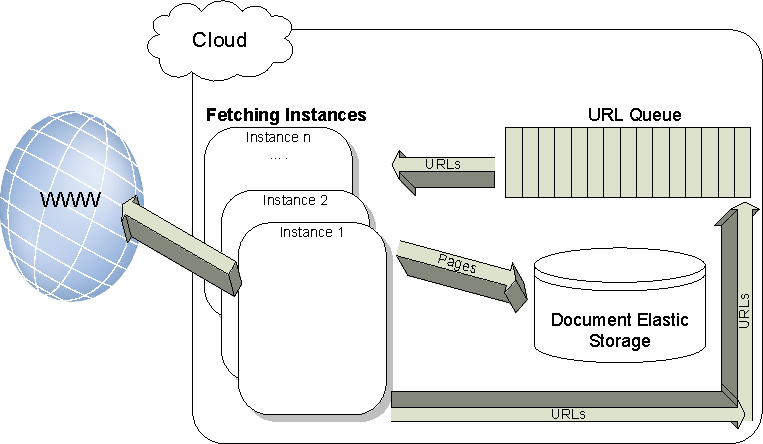
\includegraphics[width=13cm]{images/20_related/group-MC15.pdf}
    \caption[Visualisierung von Crawling Instanzen]{Visualisierung der sogenannten Crawling Instanzen innerhalb der Zielarchitektur~\parencite[vgl.][S. 4]{ElAraby2018}.}
    \label{fig:CrawlerServiceElAraby1}
\end{figure}
Der Service stellt eine Web-Crawling Lösung dar, die in Form einer einzelnen Applikation realisiert ist. Trotz der Möglichkeit zur unabhängigen Skalierung, weist die Instanz eine monolithische Architektur auf. Zusätzlich kommt ein alternativer Ansatz zur Skalierung zum Einsatz, der die Existenz mehrerer, unabhängig voneinander funktionierender URL-Queues vorsieht, wie in Abbildung \ref{fig:CrawlerServiceElArabyGlobal} dargestellt.

\begin{figure}[H]
    \centering
    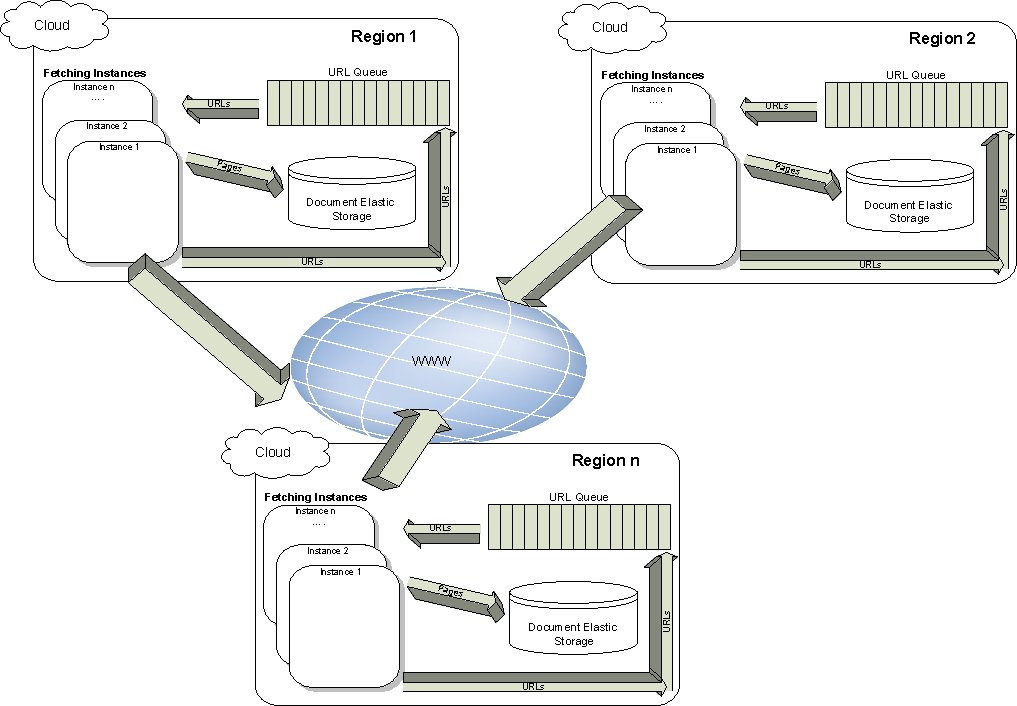
\includegraphics[width=13cm]{images/20_related/group-MC17.pdf}
    \caption[Visualisierung geographisch verteilter Crawler]{Visualisierung geographisch verteilter Crawler der Zielarchitektur~\parencite[vgl.][S. 4]{ElAraby2018}.}
    \label{fig:CrawlerServiceElArabyGlobal}
\end{figure}

Im Gegensatz zur zuvor erwähnten Arbeit mit dem Titel \textit{\citetitle{ElAraby2018}~\parencite[vgl.][]{ElAraby2018}{}{}} repräsentiert diese Arbeit eine Weiterentwicklung und konkretisiert die nächste Stufe dieser konzeptionellen Grundlage. Sie geht über die \ac{SOA} Architektur hinaus, indem sie eine noch feingliedrigere Unterteilung in unabhängige Services vornimmt. Um die aufgestellte Hypothese zu erfüllen, wird in diesem Sinne eine Microservice-basierte Architektur entwickelt.

Im Vergleich zu einer serviceorientierten Architektur, welche detailliert in Abschnitt \ref{subsec:monoservmicro} im Kontrast zu Microservices diskutiert wird, bietet letzterer Ansatz eine verbesserte Präzision und Effizienz in der Steuerung der Services. Diese Vorteile gehen jedoch mit einer gesteigerten Komplexität einher. In Abschnitt \ref{subsec:monoservmicro} werden die Vor- als auch Nachteile von Microservices nochmals umfassend beleuchtet.

In der Architektur dieser Arbeit werden nicht einzelne, gleiche Service-Instanzen eingesetzt, sondern es findet eine Synergie mehrerer, verschiedener Services statt. Darüber hinaus werden diese Microservices in einer Cloud-nativen Umgebung eingebettet. Durch die Cloud-nativen Ansätze kann nochmals eine Optimierung der Skalierbarkeit erreicht werden. Dies wird in Kapitel \ref{sec:cloudnative} beschrieben.
\section{Optimierung der Performance mit \acl{AOT}}
Im Kontext der zunehmenden Komplexität moderner Softwareentwicklung und der Notwendigkeit, diverse Technologien sowie verschiedene Programmiersprachen zu integrieren, beleuchtet der Artikel unter dem Titel \citetitle{8756917}~\parencite[vgl.][]{8756917} die Rolle der GraalVM als innovativen Ansatz. Diese Forschungsarbeit unterstreicht die Bedeutung der GraalVM für die Verbesserung der Interoperabilität zwischen Programmiersprachen bei gleichzeitiger Optimierung der Leistung. 

Der zentrale Fokus liegt auf dem in Java entwickelten Graal-Compiler, der sowohl als \ac{JIT}- als auch als \ac{AOT}-Compiler fungiert und durch seine fortgeschrittenen Optimierungstechniken, insbesondere im Hinblick auf Algorithmen, die Entwicklung und Wartung von Software beschleunigt und vereinfacht. 
\newpage
Die Arbeit hebt hervor, wie die GraalVM durch ihre Architektur und Funktionalitäten das Software-Ökosystem bereichert, indem sie eine nahtlose Integration und effiziente Ausführung von Anwendungen in verschiedenen Programmiersprachen wie Java, JavaScript, C/C++, Python, Ruby und R ermöglicht.

Das genannte Werk beleuchtet die Unterschiede zwischen \ac{AOT} und \ac{JIT} Kompilierung über verschiedene Programmiersprachen hinweg, mit einem besonderen Fokus auf die Optimierung von \ac{JVM}-basierten Sprachen. Diese Arbeit jedoch erweitert die Untersuchung, indem sie die Effektivität der Optimierung in einem praxisnahen Einsatzszenario evaluiert. Wie in \citetitle{8756917}~\parencite[vgl.][]{8756917} erwähnt, basieren die vorläufigen Testergebnisse auf einem begrenzten Umfeld, woraus der Plan entstand, die Forschung durch Experimente in einem umfangreicheren Kontext fortzusetzen.

Entsprechend knüpft die vorliegende Arbeit an dieser Stelle an, indem sie die Wirksamkeit der AOT-Optimierung in einer realitätsnahen, cloud-nativen Umgebung untersucht, in der die Anwendungen integriert sind. Die Untersuchung erstreckt sich dabei auf einen Bereich, in dem bisher wenig Forschung vorliegt: den spezifischen Anwendungskontext von Web-Crawling.

Diese Arbeit zielt darauf ab, diese Lücke zu schließen, indem sie die Anwendbarkeit und Vorteile der \ac{AOT}-Optimierung für Web-Crawling in einer Cloud-nativen Umgebung untersucht. Die Analyse konzentriert sich auf die Herausforderungen und Anforderungen, die für das Web-Crawling spezifisch sind. 

\vfill

\chapterend        % research related (to your!) work 
%\include{chapters/30_background}    % if necessary, explain possilby unknown terms or technologies used
%%%%%%%%%%%%%%%%%%%%%%%%%%%%%%%%%%%%%%%%%%%%%%%%%%%%%%%%%%%%%%%%%%%%%%%%%%%%%
\chapter{Konzept}
\label{chap:concept}
%%%%%%%%%%%%%%%%%%%%%%%%%%%%%%%%%%%%%%%%%%%%%%%%%%%%%%%%%%%%%%%%%%%%%%%%%%%%%
\chapterstart

Um eine Optimierung der Skalierbarkeit sowie der Ressourceneffizienz eines Web-Crawlers durchzuführen, ist eine fundierte Konzeptionierung essenziell. Im nachstehenden Kapitel wird auf traditionelle Web-Crawling Konzepte eingegangen. Diese werden beleuchtet und wichtige Erkenntnisse zusammengefasst, die im Folgenden in die Konzeption einer optimierten Variante einfließen. 

Im Subkapitel \textit{\nameref{sec:cloudnative}} werden zunächst Konzepte zur Unterstützung der Hypothese \textit{\nameref{subsec:hypothesis:scalability}} untersucht. Das Kapitel gibt einen Überblick über die Cloud-native Landschaft und ihren Prinzipien. Mit diesen Erkenntnissen wird in Kapitel \ref{subsec:microservicekontextcrawler} eine Optimierung eines traditionellen Web-Crawling Ansatzes durchgeführt.

Das darauffolgende Kapitel, betitelt als \textit{\nameref{sec:aot}}, befasst sich mit dem Konzept der \ac{AOT} und dessen Bedeutung in Bezug auf die Verbesserung von Web-Crawling Methoden. Zunächst wird die Definition der \acl{AOT} vorgestellt, gefolgt von einer detaillierten Gegenüberstellung dieser mit der \acl{JIT}. Diese Gegenüberstellung ermöglicht eine tiefgreifende Analyse der Vor- und Nachteile beider Ansätze. Abschließend wird untersucht, wie die \acl{AOT} spezifisch in den Web-Crawling Kontext integriert werden kann, um die Leistung und Effizienz des Crawling-Prozesses zu verbessern.
\section{Traditionelle Web-Crawling Konzepte}\label{sec:traditionalconcepts}
Im Bereich des Web-Crawling existieren verschiedene Techniken, die dazu dienen, spezifische Herausforderungen in diesem Bereich erfolgreich zu bewältigen. Einige der Herausforderungen, denen Web-Crawling gegenübersteht, könnten beispielsweise die effiziente Verwaltung von großen Datenmengen, die Überwindung von Zugriffsbeschränkungen auf bestimmten Webseiten, die Erkennung und Handhabung von dynamisch generierten Inhalten sowie die effektive Navigation durch komplexe Strukturen von Webseiten sein. 

Eine allgemeine Unterteilung definiert das Werk \citetitle{sharma2015anatomy}~\parencite[vgl.][S. 1-3]{sharma2015anatomy}{}{}. In diesem Werk werden vier verschiedene Typen von Web-Crawlern erwähnt und miteinander verglichen, welche nachstehend erläutert werden:

\begin{itemize}
    \item \textbf{Parallel-Crawlers}: Diese Crawler arbeiten gleichzeitig mit mehreren Instanzen, um große Teile des Web effizient zu durchsuchen.
    \item \textbf{Focused-Crawlers}: Diese sind auch bekannt als ''Thematische-Crawler'' oder ''Topical-Crawler'' und konzentrieren sich vor allem auf spezifische Inhalte oder Themengebiete. Durch den Einsatz von Klassifikatoren und die Priorisierung von Links, die zu themenrelevanten Ressourcen führen, verbessern sie die Effizienz der Datensammlung in Bezug auf ein spezifisches Interessengebiet.
    
    \item \textbf{Incremental-Crawler}: Diese Crawler zielen darauf ab, die bereits untersuchten Inhalte aktuell zu halten, indem sie das Web kontinuierlich durchsuchen und periodisch bereits untersuchte Seiten erneut besuchen. Sie berücksichtigen die Änderungshäufigkeit und Wichtigkeit der Seiten.
    
    \item \textbf{Hidden-Crawler}: Sie sind darauf spezialisiert, Inhalte zu erfassen, welche hinter Suchformularen oder Bereichen verborgen und durch bereits erwähnte Web-Crawler nicht erreichbar sind. Diese Crawler interagieren mit Webformularen und sammeln Daten aus Datenbanken, die erst nach einer Formularübermittlung zugänglich werden.
\end{itemize}

Durch die gezielte Anwendung dieser Techniken lassen sich diverse Ansätze für eine Architektur ableiten. Im speziellen Kontext des Web-Crawlings ist das übergeordnete Ziel stets die Entwicklung eines höchst optimierten Architekturansatzes. Hierbei spielen Effizienz, Leistungsfähigkeit und Skalierbarkeit eine zentrale Rolle. Es gilt, eine Architektur zu gestalten, die den spezifischen Anforderungen des Web-Crawlings gerecht wird und dabei maximale Effektivität gewährleistet.
\newline
In der Regel beruhen Crawling-Systeme auf einem gemeinsamen Grundprinzip, welches in Abbildung \ref{fig:architecture-general} visualisiert wird.
\begin{figure}[H]
    \centering
    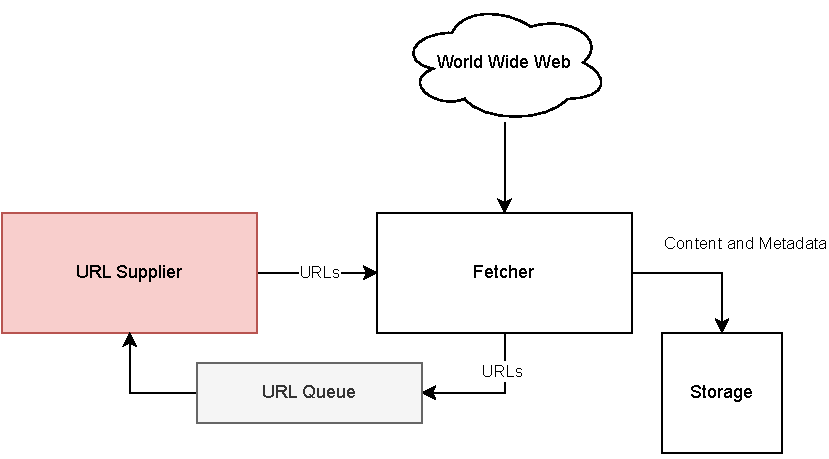
\includegraphics[width=14cm]{images/40_concept/HighLevelArch.pdf}
    \caption[Übersicht der Web-Crawler Basisarchitektur]{Übersicht der Web-Crawler Basisarchitektur bestehend aus URL-Supplier, Fetcher, URL-Queue sowie Storage.}
    \label{fig:architecture-general}
\end{figure}

Dieses grundlegende Prinzip basiert auf mehreren Komponenten, die miteinander interagieren. Der schematisch dargestellte \textbf{\textit{''URL-Supplier''}} führt die initiale Versorgung von Start-URLs durch, welche dann vom \textbf{\textit{''Fetcher''}} übernommen werden – dem Softwarebaustein, der den Download und das Verarbeiten des Inhalts durchführt. Unter Verarbeitung versteht man oft eine Filterung der URLs, bevor sie an eine weitere Komponente weitergegeben werden. Die abgerufenen Daten werden daraufhin in einer Datenbank gespeichert. Durch eine Auswertung des Inhalts, den der \textbf{\textit{''Fetcher''}} heruntergeladen hat, werden URLs gemäß bestimmter Regeln extrahiert. Diese extrahierten URLs gelangen dann in die \textbf{\textit{''URL-Queue''}}, wo sie vom \textbf{\textit{''Supplier''}} erneut weiterverarbeitet werden. Somit entsteht ein geschlossener Prozess.

Auf Basis dieses schematischen Prinzips wird nun eine skalierbare und effiziente Lösung entwickelt, um die in Kapitel \ref{sec:problem} angeführte Problemstellung zu adressieren. In den nachfolgenden Abschnitten, insbesondere in Kapitel \ref{sec:cloudnative} und \ref{sec:aot}, wird ein konkretes Konzept ausführlich erörtert.
\section{Einbettung in die Cloud-native Landschaft} \label{sec:cloudnative}
Der Cloud-native-Ansatz und die 12-Faktor-App-Methode sind zwei Konzepte, die eng miteinander verbunden sind und die Entwicklung von Anwendungen für die Cloud unterstützen. Der Cloud-native-Ansatz bezieht sich auf die Entwicklung von Anwendungen, die speziell für den Betrieb in einer Cloud-Umgebung optimiert sind. 
Die \textit{\ac{CNCF}} definiert den Begriff \textit{''Cloud-Native''}, um die Kernprinzipien - Skalierbarkeit, lose Kopplung, Resilienz, Observability und Manageability - zu vermitteln:

\begin{spar}
\textit{Cloud native technologies empower organizations to build and run scalable applications in modern, dynamic environments such as public, private, and hybrid clouds. Containers, service meshes, microservices, immutable infrastructure, and declarative APIs exemplify this approach.~\parencite[][]{CNCF}}
\end{spar}


Die 12-Faktor-App-Methode hingegen stellt eine Sammlung von Prinzipien und bewährten Vorgehensweisen dar, die bei der Entwicklung von Cloud-nativen Anwendungen befolgt werden sollte~\parencite[vgl.][]{12Factor}.
Zusammengefasst beinhaltet die 12-Faktor-App-Methode folgende Charakteristiken: 

\begin{spar}
\textit{Suitable to be deployed on cloud platforms, Scalable by design, Portable across systems, Enablers of continuous deployment and agility.~\parencite[][S. 36]{vitale}}
\end{spar}

Die skizzierten Prinzipien können in einer Web-Crawling Architektur ebenso Anwendung finden. In den nachfolgenden Abschnitten werden diese Prinzipien ausführlich behandelt und in den spezifischen Kontext des Web-Crawling eingebunden.

\subsection{Softwarearchitekturen in verteilten Systemen} \label{subsec:monoservmicro}
Wenn das Ziel darin besteht, eine Anwendung in eine Cloud-native Umgebung zu integrieren, um die Vorteile dieses Ansatzes voll auszuschöpfen, wird es früher oder später erforderlich sein, sich mit der Frage auseinanderzusetzen, welcher geeignete Softwarearchitekturansatz in diesem spezifischen Kontext am besten geeignet ist. In diesem Werk werden insbesondere die folgenden Ansätze beleuchtet: \textbf{\acl{SOA}} sowie \textbf{Microservice-Architektur.}\newline\newline
\textbf{\acl{SOA}}\newline
Serviceorientierung beschreibt eine sogenannte Basisarchitektur und definiert laut dem Werk \citetitle{Gharbi_Koschel_Rausch_Starke_2023}~\parencite[vgl.][]{Gharbi_Koschel_Rausch_Starke_2023}{}{} verteilte sowie lose gekoppelte Dienste. Diese Dienste stellen Schnittstellen bereit, über die Interaktionen ausgeführt werden können. Diese Interaktionen sollten in Form eines Vertrags zwischen dem Dienstanbieter und dem Dienstnutzer erfolgen. Diese Services sind eigenständige, wiederverwendbare Softwarekomponenten, die spezifische Funktionen bereitstellen. Sie ermöglichen eine Modularisierung und fördern die Wiederverwendbarkeit und Austauschbarkeit, da eine klar definierte Schnitstelle zwischen den Vertragspartnern existiert.\newline\newline
\textbf{Microservice-Architektur}\newline
    Die Microservice-Architektur ist laut \citetitle{Wolff_2018}~\parencite[vgl.][S. 6]{Wolff_2018} eine weitere Herangehensweise an die Entwicklung von Softwareanwendungen, bei der eine Anwendung in kleinere, unabhängige Dienste (Microservices) aufgeteilt wird. Der zuvor beleuchtete Ansatz der Serviceorientierung dient als Grundlage dafür. Jeder Microservice ist für einen klar definierten Teil der Funktionalität verantwortlich und kann eigenständig entwickelt, bereitgestellt und skaliert werden.

In der Arbeit von \citetitle{Wolff_2018}~\parencite[vgl.][S. 14-17]{Wolff_2018} werden die Vor- und Nachteile von Microservices umfassend diskutiert. Im nachstehenden Absatz werden die Schlüsselaspekte dieser Diskussion extrahiert und kurz erläutert. Darauf folgt eine detaillierte Analyse dieser Aspekte speziell im Rahmen des Web-Crawlings, wie in Abschnitt \ref{subsec:microservicekontextcrawler} näher ausgeführt wird.

    \textbf{Vorteile von Microservices:}
    \begin{itemize}
      \item \textbf{Getrennte Datenhaushalte:} Jeder Microservice verwaltet seine eigenen Daten, was die Änderbarkeit der Software erleichtert.
            
      \item \textbf{Flexibilität bei der Technologiewahl:} Jeder Microservice kann in einer anderen Technologie implementiert werden.

      \item \textbf{Unabhängige Skalierbarkeit:} Microservices ermöglichen eine gezielte Skalierung spezifischer Dienste, was die Ressourcennutzung effizienter macht.


    \end{itemize}
    
    \textbf{Nachteile von Microservices:}
    \begin{itemize}
      \item \textbf{Erhöhte Systemkomplexität:} Die Nutzung verschiedener Technologien erhöht die Gesamtkomplexität des Systems.
      
      \item \textbf{Verwundbarkeit in verteilten Systemen:} Microservices sind anfälliger\newline für Netzwerk- und Serverausfälle.
      
      \item \textbf{Architektonische Herausforderungen:} Die Aufteilung in Microservices kann zu unbeabsichtigten Abhängigkeiten führen.
    \end{itemize} 



\subsection[Analyse Microservice im Anwendungskontext]{Analyse Architekturmuster Microservice im Anwendungskontext}\label{subsec:microservicekontextcrawler}
Nachdem einige relevante Vor- und Nachteile von Microservices, basierend auf das Werk  \citetitle{Wolff_2018}~\parencite[vgl.][S. 14-17]{Wolff_2018}, betrachtet wurden, richtet sich der Fokus nun auf die Anwendung dieser Architektur im Bereich des Web-Crawlings, insbesondere im Hinblick auf die Skalierungseffizienz. Dieser Abschnitt konzentriert sich auf die Merkmale der Microservice-Architektur, die direkt die Skalierbarkeit und die damit verbundenen Herausforderungen beeinflussen. In den folgenden Abschnitten wird untersucht, wie diese spezifischen Eigenschaften von Microservices die Leistungsfähigkeit und Effizienz im Kontext des Web-Crawlings verbessern oder beeinträchtigen können.


\textbf{Loose Kopplung einzelner Services im Kontext von Web-Crawling}

Loose Kopplung stellt ein fundamentales Konzept innerhalb der\newline Microservice-Architektur dar, das im Bereich des Web-Crawlings eine zentrale Rolle einnimmt. Diese Eigenschaft ermöglicht es, diverse Aufgaben, die während des Crawling-Prozesses entstehen, flexibel zu managen.

Indem die Komponenten des Web-Crawling-Prozesses, wie das Abrufen von Webseiten, das Parsen von Inhalten und die Datenextraktion, in unabhängigen Microservices implementiert werden, erhöht sich die Autonomie jeder Komponente. Diese Modularität fördert nicht nur die Wartbarkeit und Fehlertoleranz durch die Isolation von Störungen in einzelnen Komponenten, sondern trägt auch zur Systemresilienz bei, indem es die Auswirkungen von Ausfällen minimiert. Dies ist besonders relevant in Umgebungen, in denen die Interaktion mit einer Vielfalt von Webseiten unvorhersehbare Fehler generieren kann.

\textbf{Unabhängige Skalierbarkeit im Kontext von Web-Crawling}

Unabhängige Skalierbarkeit, ein weiteres zentrales Prinzip der \newline Microservice-Architektur, ist im Web-Crawling essentiell. Diese Fähigkeit, einzelne Microservices bedarfsorientiert zu skalieren, ohne andere Systemkomponenten zu beeinträchtigen, ist entscheidend für die effiziente Ressourcen- und Leistungsverwaltung. Spezifische Dienste, verantwortlich für Crawling, Parsen oder Datenextraktion, können entsprechend den vorliegenden Anforderungen angepasst werden, was eine flexible Reaktion auf dynamische Lastsituationen ermöglicht.

\textbf{Zusammenspiel von loser Kopplung und unabhängiger Skalierbarkeit}

Die Integration von loser Kopplung und unabhängiger Skalierbarkeit in der Architektur von Web-Crawling-Systemen schafft signifikante Vorteile. Durch die lose Kopplung operieren Microservices als selbstständige Einheiten, was eine Prämisse für deren unabhängige Skalierung bildet.

Beispielsweise ermöglicht es die Architektur, den für das Parsen zuständigen Microservice separat zu skalieren, sollte dieser aufgrund eines erhöhten Datenaufkommens oder komplexer Inhaltsstrukturen unter Last stehen, unabhängig von anderen Services wie Datenextraktion oder Speicherung. So bleibt die Gesamtperformance des Crawling-Systems stabil, selbst wenn einzelne Komponenten spezifischen Herausforderungen gegenüberstehen.

\subsection{Eventbasierte vs Synchrone Inter-Service-Kommunikation}\label{subsec:eventdriven}
Im nachfolgenden Abschnitt erfolgt eine vergleichende Analyse zwischen eventbasierter und synchroner Kommunikation bei Services, welche das Ziel verfolgen, eine theoretische Grundlage für die weitere Konzeptionierung zu etablieren.

Eventbasierte Kommunikation in verteilten Systemen benötigt zwei Hauptkomponenten für den Nachrichtenaustausch zwischen Diensten. Die folgende Definition der Komponenten basiert auf dem Werk \citetitle{vitale}~\parencite[vgl.][]{vitale}{}{}.

\begin{enumerate}
    \item \textbf{Message-Broker}: vermittelt Nachrichten zwischen Sendern und Empfängern
    \item \textbf{Übertragungsprotokoll}: regelt die Datenübertragung zwischen\newline Sendern und Empfängern
\end{enumerate}

Die Kombination eines Message-Brokers mit einem dedizierten Übertragungsprotokoll ermöglicht asynchrone Kommunikation. Dabei müssen Anfragen und Antworten nicht sequenziell verarbeitet werden, sondern können unabhängig und basierend auf Verfügbarkeit bearbeitet werden. Die Vorteile dieses Ansatzes definiert \citetitle{vitale}~\parencite[vgl.][]{vitale}{}{} wie folgt:

 \begin{itemize}
  \item \textbf{Entkopplung der Service-Prozesse:} Services sind nicht gezwungen, auf direkte Antworten zu warten, wodurch Verzögerungen minimiert werden. 
  \item \textbf{Erhöhte Fehlertoleranz:} Bei Ausfall eines Services werden Nachrichten in der Warteschlange gehalten und gehen nicht verloren.
  \item \textbf{Skalierbarkeit:} Die asynchrone Verarbeitung ermöglicht eine bessere Skalierbarkeit, da Services unabhängig und parallel arbeiten können, ohne durch Synchronisationsprobleme eingeschränkt zu werden.
\end{itemize}

\ac{AMQP}, ein weit verbreitetes Übertragungsprotokoll, bietet vor allem durch zuverlässige Nachrichtenübermittlung und Interoperabilität zwischen Plattformen signifikante Vorteile \parencite[vgl.][]{vitale}. Bei dieser spielen sogenannte \textbf{''Event-Producer''} sowie \textbf{''Event-Consumer''} eine zentrale Rolle. Der Producer, so definiert es auch \citeauthor{vitale}~\parencite[vgl.][]{vitale}, ist dafür zuständig, Nachrichten zu versenden, hingegen der Consumer Nachrichten entgegennimmt. Dabei agieren Producer und Consumer unabhängig voneinander und haben keine direkte Verbindung zueinander. Visualisiert wird dies in Abbildung \ref{fig:amqp}.  
 
\begin{figure}[H]
    \centering
    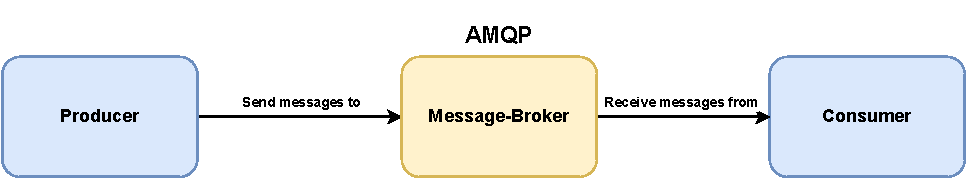
\includegraphics[width=14.5cm]{images/40_concept/AMQP.drawio.pdf}
    \caption[Visualisierung \acl{AMQP} Teilnehmer]{Visualisierung der Interaktion zwischen Event-Producer, Message-Broker und Event-Consumer in \ac{AMQP}~\parencite[vgl.][]{vitale}.}
    \label{fig:amqp}
\end{figure}
 Vor allem in Bezug auf die Zuverlässigkeit wird das verwendete Übertragungsprotokoll \ac{AMQP} relevant. So untersucht die Studie \textit{\citetitle{9023812}~\parencite[vgl.][]{9023812}{}{}} Alternativen, wie beispielweise \ac{MQTT}. Die Studie hebt hervor, dass \ac{AMQP} insbesondere in Szenarien mit hohen Anforderungen an die Zuverlässigkeit und Sicherheit der Datenübertragung überlegen ist. Die erwähnte Studie fokussiert sich zwar auf Anwendungen im Bereich ''Internet of Things'', jedoch lassen sich die Ergebnisse durchaus für weiterführende Forschung verwenden.

  Im Konzept dieser Arbeit sind Producer und Consumer zwei unterschiedliche Microservices. Ein RabbitMQ-Server fungiert als Message-Broker. Dieser Message-Broker wurde ausgewählt, da RabbitMQ sich durch die Verwendung von \ac{AMQP} auszeichnet. Eine empirische Analyse zwischen \ac{AMQP}-Message-Brokern bietet die Arbeit mit dem Titel \citetitle{9615705}~\parencite[vgl.][]{9615705}{}{}. In diesem wird RabbitMQ mit ActiveMQ, einer weiteren Implementierung eines Message-Brokers, verglichen. Durch diese Arbeit wird aufgezeigt, dass ActiveMQ zwar im Vergleich zum verwendeten RabbitMQ einen höheren Durchsatz an Nachrichten erlaubt, jedoch RabbitMQ eine geringere Latenz aufweist. Diese geringere Latenz wird in Abbildung \ref{fig:RABACTIVE} ersichtlich. Aufgrund der Optimierung der Durchlaufzeit des Prototyps wurde explizit ein Message-Broker mit einer geringen Latenz gewählt und der geringere Durchsatz mit einer optimierten Struktur des Nachrichten ausgeglichen. Dies ist in Kapitel \ref{subsec:eventbas} ersichtlich.

  \begin{figure}[H]
    \centering
    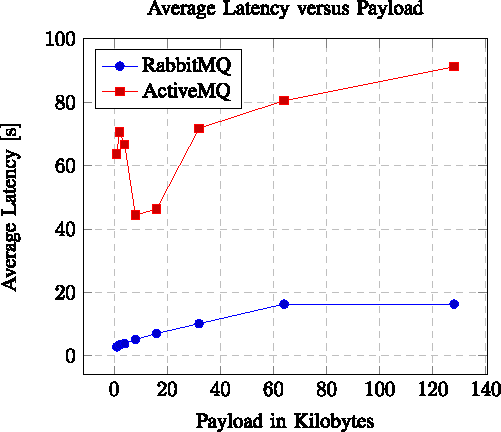
\includegraphics[width=10cm]{images/40_concept/Performance_Evaluation_of_Advanced_Message_Queuing_Protocol_AMQP_An_Empirical_Analysis_of_AMQP_Online_Message1_Brokers.pdf}
    \caption[Empirischer Vergleich zwischen ActiveMQ und RabbitMQ]{Empirischer Vergleich zwischen ActiveMQ und RabbitMQ in Bezug auf Latenz und Nachrichtengröße~\parencite[vgl.][]{9615705}{}{}.}
    \label{fig:RABACTIVE}
\end{figure}
Die Alternative zu einem asynchronen bzw. eventbasierten Ansatz wäre ein synchroner Datenaustausch, bei dem jede Anfrage eine unmittelbare Antwort erfordert, bevor der nächste Schritt erfolgen kann. Dies kann zu Engpässen führen, insbesondere in Systemen mit hoher Last, da der Verarbeitungsfluss durch die Antwortzeiten der einzelnen Services begrenzt wird. Im Gegensatz zum synchronen Datenaustausch führt ein eventbasiertes Verfahren jedoch zu einer erhöhten Komplexität, was unter anderem auch in Kapitel \ref{subsec:eventbas} verdeutlicht wird. In einem Web-Crawling Kontext, wo schnelle und effiziente Datenverarbeitung kritisch ist, könnte ein synchroner Ansatz aber die Leistungsfähigkeit des Gesamtsystems erheblich beeinträchtigen.

\subsection[Konzeptionierung Microservice im Anwendungskontext]{Konzeptionierung Architekturmuster Microservice im Anwendungskontext}
Die architektonische Übersicht in Abbildung \ref{fig:architecture} bietet einen umfassenden Überblick über die grundlegende Struktur der Softwareanwendung. Sie stellt die verschiedenen Hauptkomponenten und ihre Interaktionen dar. Diese Übersicht dient als Ausgangspunkt für die weitere Planung und Entwicklung der Anwendung und wird in diesem Kapitel genauer beschrieben.

\begin{figure}[H]
    \centering
    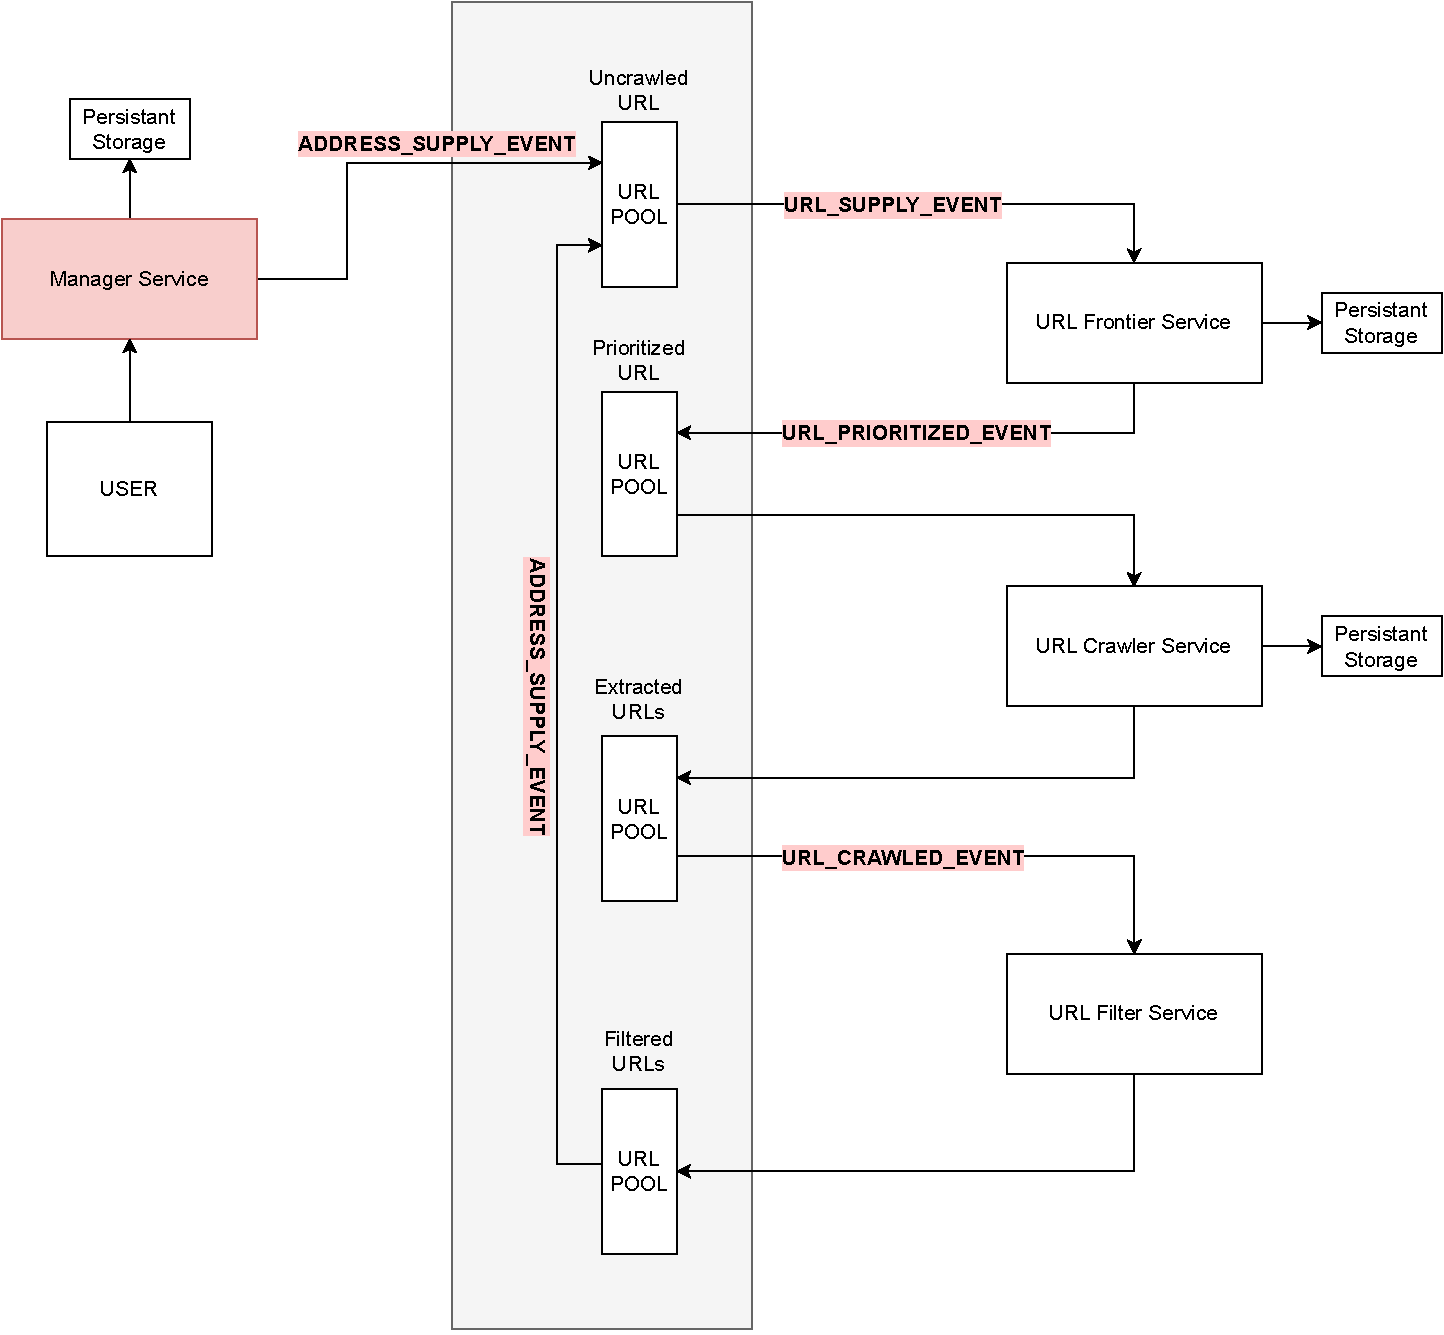
\includegraphics[width=14cm]{images/40_concept/microservice_conception.pdf}
    \caption[Visualisierung Web-Crawler Basisarchitektur]{Visualisierung der Aufteilung von einer Web-Crawler Basisarchitektur in Microservices samt Kommunikationsfluss.}
    \label{fig:architecture}
\end{figure}

Innerhalb der Architektur des Web-Crawlers nehmen sekundäre Services eine essenzielle Funktion ein. Diese Services verarbeiten eingehende Anfragen, die entweder direkt von Benutzern oder von anderen Servicekomponenten initiiert werden, und leiten die Ergebnisse entsprechend weiter. Ein kritisches Designprinzip, welches in Abschnitt \ref{subsec:microservicekontextcrawler} diskutiert wird, ist die lose Kopplung zwischen den einzelnen Microservices. Obwohl Interaktionen zwischen den Services sowohl möglich als auch erforderlich sind, ist eine direkte Abhängigkeit zu vermeiden. Aus diesem Grund wurde, wie in Abschnitt \ref{subsec:eventdriven} beschrieben, RabbitMQ als robustes Werkzeug für die Kommunikation zwischen den Services ausgewählt. Dies ermöglicht eine effiziente und zuverlässige Interaktion und unterstützt somit die Skalierbarkeit.
\newpage
Aufbauend auf den in Kapitel \ref{sec:traditionalconcepts} besprochenen traditionellen Konzepten, wurden spezifische Microservices für den Web-Crawler definiert. Diese Microservices sind:

\begin{itemize}
    \item \textbf{Manager Service:} Dieser Service fungiert als zentrale Steuerungseinheit, koordiniert die Aktivitäten der anderen Services und überwacht den Gesamtzustand des Crawling-Prozesses.
    \item \textbf{Frontier Service:} Verantwortlich für die Verwaltung der Crawling-Frontier, speichert dieser Service Informationen über zu besuchende URLs und priorisiert sie entsprechend.
    \item \textbf{Crawler Service:} Dieser Service führt das eigentliche Crawling durch, indem er Webseiten abruft und deren Inhalte extrahiert.
    \item \textbf{Filter Service:} Er filtert und bereinigt die extrahierten Daten, um sicherzustellen, dass nur relevante und qualitativ hochwertige Informationen für die weitere Verarbeitung verwendet werden.
\end{itemize}

Jeder dieser Services ist für einen spezifischen Aspekt des Web-Crawlings zuständig und trägt eine entscheidende Funktion zum Gesamtsystem bei. Im folgenden Kapitel wird eine detaillierte Aufgabenbeschreibung der einzelnen Services gegeben, um ihre Funktion ersichtlich zu machen. In der Grafik werden die Messages explizit hervorgehoben, welche über den Message-Broker ein- und ausgehen.

\noindent\rule{\textwidth}{1pt}

\textbf{Konzeption Manager Service}\newline
\textbf{Message-Queue Output:} Seed-URLs\newline
\begin{figure}[H]
    \centering
    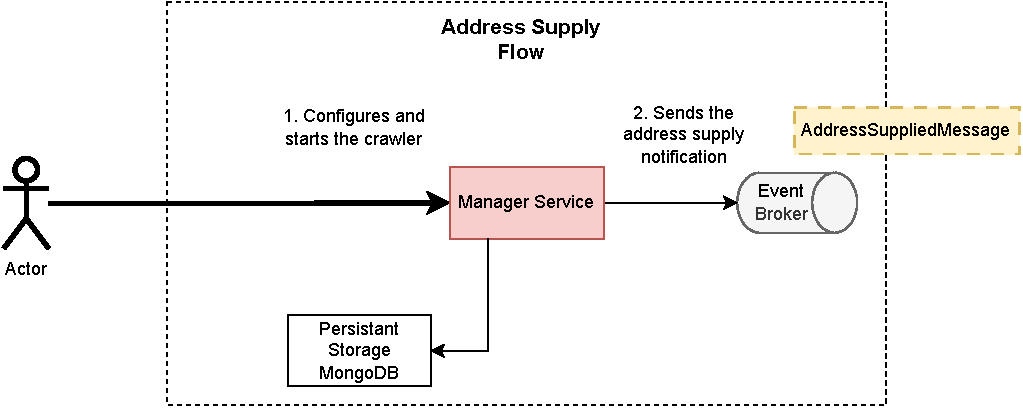
\includegraphics[width=14cm]{images/40_concept/ManagerService.drawio.pdf}
    \caption[Detailansicht des Manager Services]{Detailansicht des Manager Services samt Message-Queue-Interaktion sowie Darstellung der Benutzerschnitstelle.}
    \label{fig:ManagerService}
\end{figure}

Der Manager Service (siehe Abbildung \ref{fig:ManagerService}) ist für die Verwaltung von \newline Crawler-Konfigurationen zuständig und realisiert die entsprechenden Create-, Read-, Update- und Delete-Operationen. Dies ermöglicht es, Crawler-Konfigurationen zu erstellen, zu lesen, zu aktualisieren und zu entfernen. Zusätzlich ist der Manager Service dafür verantwortlich, Crawling-Prozesse zu initiieren und zu terminieren.

Die Konfigurationsdaten sowie der Status der Crawler werden in einer MongoDB-Datenbank persistiert. Die Wahl einer dokumentenbasierten Datenbank wie MongoDB ermöglicht Flexibilität in der Datenspeicherung, insbesondere durch die Fähigkeit, dynamisch neue Felder zu den Dokumenten hinzuzufügen, ohne die Struktur bestehender Datensätze zu beeinträchtigen.
Beim Start eines Crawlers generiert der Manager Service ein \textbf{\textit{AddressSuppliedMessage-Event}}, das über einen Event-Broker weitergeleitet wird. Dieses Ereignis enthält die initialen URLs für den Crawler, auch Seed-URLs genannt, und markiert den Beginn des Crawling-Prozesses. Der nachfolgende Service in der Verarbeitungskette, beispielsweise der Frontier Service, empfängt dieses Ereignis und setzt den Crawling-Prozess mit den bereitgestellten URLs fort.

Durch die beschriebene Funktionsweise agiert der Manager Service als zentrale Schnittstelle für die Steuerung und Überwachung der Crawler-Konfigurationen und -Status, wobei der Informationsfluss über definierte Ereignisse und die Speicherung von Zustandsinformationen in der Datenbank die Interoperabilität zwischen verschiedenen Services sicherstellt.\newline
\noindent\rule{\textwidth}{1pt}
\textbf{Konzeption Frontier Service}
\newline
\textbf{Message-Queue Input:} Seed-URLs bzw. gefilterte URLs\newline
\textbf{Message-Queue Output:} Priorisierte URLs\newline
\begin{figure}[H]
    \centering
    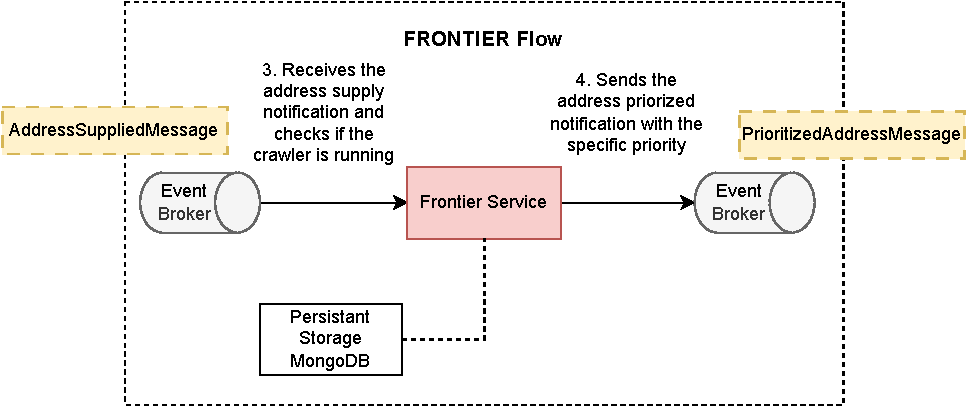
\includegraphics[width=14cm]{images/40_concept/FrontierService.drawio.pdf}
    \caption[Detailansicht des Frontier Services]{Detailansicht des Frontier Services samt Message-Queue-Interaktion.}
    \label{fig:FrontierService}
\end{figure}

Der Frontier Service (siehe Abbildung \ref{fig:FrontierService}) ist für die sogenannte \textbf{\textit{''Deduplication''}} der zu untersuchenden bzw. erhaltenen URL-Liste zuständig. Diese URL-Liste wurde entweder vom User als Seed-URL konfiguriert und vom Manager Service gesendet oder stammt von einem vorangegangenen Crawling-Prozess, bei dem der Filter Service die URLs normalisiert, gefiltert und weitergeleitet hat. Dieser Ansatz ist ein wichtiger Baustein und wird auch im bereits erwähnten Kapitel \textit{\nameref{sec:traditionalconcepts}} umgesetzt. So ist diese Funktion für einen vergleichbaren Prototypen essentiell. Er empfängt Seed-URLs bzw. extrahierte URLs vom Message-Broker, wie in Abbildung \ref{fig:FrontierService} dargestellt, und wählt diese für das Crawling aus. 

Der Frontier Service dient als primärer Knotenpunkt für den Beginn des Crawling-Prozesses und ist zuständig für die bereits erwähnte \textbf{\textit{''Deduplication''}} bzw. dem Aussortieren von URLs, die bereits verarbeitet wurden. Die Informationen zu bereits gecrawlten URLs werden in einer MongoDB gespeichert. Bereits gecrawlte URLs werden in diesem Vorgang nicht mehr gespeichert. Vor der Weiterleitung einer URL zum Crawling prüft der Frontier Service in dieser Datenbank, ob die betreffende URL bereits gecrawlt wurde. Sollte eine URL bereits verarbeitet worden sein, wird sie vom weiteren Crawling-Prozess ausgenommen, um Doppelarbeit zu verhindern. Der Frontier Service trägt somit die Verantwortung, sicherzustellen, dass keine URL mehrfach gecrawlt wird, und kann gegebenenfalls den Crawling-Vorgang für bereits analysierte Webseiten erneut initiieren. Nach dieser \textbf{\textit{''Deduplication''}} werden diese an den Event-Broker weitergeleitet.

\noindent\rule{\textwidth}{1pt}

\textbf{Konzeption Crawler Service}
\newline
\textbf{Message-Queue Input:} Vom Frontier-Service priorisierte URLs \\
\textbf{Message-Queue Output:} Liste der ungefilterten URLs

\begin{figure}[H]
    \centering
    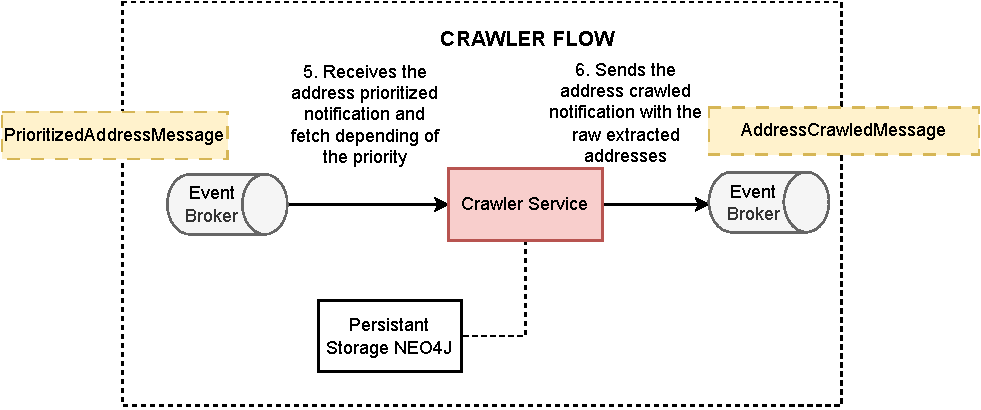
\includegraphics[width=14cm]{images/40_concept/CrawlerService.drawio.pdf}
    \caption[Detailansicht des Crawler Services]{Detailansicht des Crawler Services samt Message-Queue-Interaktion.}
    \label{fig:CrawlerService}
\end{figure}

Der Crawler Service (siehe Abbildung \ref{fig:CrawlerService}) ist ein entscheidender Bestandteil des \newline Crawling-Prozesses, der sich primär auf das Herstellen von Verbindungen zu Webservern und das Extrahieren von URLs konzentriert. 

Die primäre Funktion des Crawler Service ist das Etablieren von Verbindungen zu den Webservern der bereitgestellten URLs und das Abrufen der Webseiteninhalte. Dabei werden Techniken wie das Konfigurieren von Request-Headern, das Festlegen von Timeouts und das Implementieren von Wiederholungsmechanismen bei Verbindungsfehlern angewandt, um eine effiziente und fehlerresistente Datenakquisition zu gewährleisten.

Nach dem Herunterladen der Webseiteninhalte folgt die Analyse und das Extrahieren von URLs aus dem erhaltenen Webinhalt. Diese extrahierten URLs werden in einer strukturierten Nachricht, der \textbf{\textit{AddressCrawledMessage}}, gesammelt und für den nächsten Verarbeitungsschritt, beispielsweise dem Filter-Service, zur Verfügung gestellt.

Zudem ist der Crawler Service für die Persistenz der gewonnenen Daten zuständig. Die extrahierten URLs werden in einer Neo4j-Datenbank gesichert. Innerhalb dieser Graph-Datenbank werden die Webseiten als Knoten abgebildet und über Edges mit anderen gecrawlten Webseiten vernetzt, was die Analyse der Webstruktur ermöglicht und die Abfrageeffizienz steigert.

Der Manager Service bietet ein Konfigurationsobjekt, genannt \textit{\textbf{Actions}}, für die Indexierung der durch den Crawler Service erfassten Daten einer Webseite. Dieses Konfigurationsobjekt ermöglicht die Definition spezifischer Regeln, die festlegen, unter welchen Bedingungen ein bestimmter Index einer in der Datenbank gespeicherten Entität zugewiesen wird. Eine solche Aktion kann beispielweise einen Index auf eine Entität setzen, wenn eine bestimmte Zeichenfolge im Inhalt einer Webseite gefunden wird. In diesem Fall weist der Crawler Service der betreffenden Entität einen Index zu, um sie entsprechend zu markieren.

\noindent\rule{\textwidth}{1pt}
\newpage
\textbf{Konzeption Filter Service} \newline
\textbf{Message-Queue Input:} Liste der ungefilterten URLs\\
\textbf{Message-Queue Output:} Liste der gefilterten URLs

\begin{figure}[H]
    \centering
    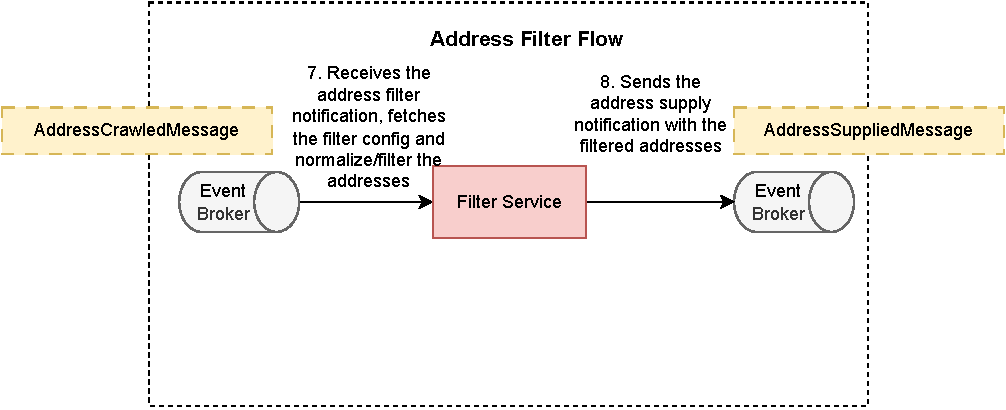
\includegraphics[width=14cm]{images/40_concept/FilterService.drawio.pdf}
    \caption[Detailansicht des Filter Services]{Detailansicht des Filter Services samt Message-Queue-Interaktion.}
    \label{fig:FilterService}
\end{figure}

Der Filter Service (siehe Abbildung \ref{fig:FilterService}) ist für die Normalisierung und Filterung der vom Crawler Service bereitgestellten URLs zuständig. Er transformiert die ungefilterten URLs in ein einheitliches Format und wendet festgelegte Filterkriterien an, um sicherzustellen, dass nur relevante Adressen für den weiteren Verarbeitungsprozess selektiert werden.

Im Normalisierungsprozess werden URLs gemäß definierten Regeln umgewandelt, um Konsistenz zu erreichen. Diese Normalisierung ist entscheidend, um eine effiziente Weiterverarbeitung durch andere Services im System zu gewährleisten.

Der anschließende Filterungsprozess prüft jede URL anhand einer konfigurierbaren Menge von Regeln und Kriterien. Diese Regeln können die Einschränkung auf bestimmte Domänen, Pfade oder Parameter beinhalten. URLs, die diesen Filterkriterien nicht entsprechen, werden eliminiert. Die entsprechende Filterkonfiguration wird durch den Manager-Service vorgegeben.

Abschließend werden die qualifizierten, gefilterten URLs an den Frontier Service übergeben, wodurch der Crawling-Zyklus erneut initiiert wird. Dieser Prozess stellt sicher, dass der Crawler nur auf URLs fokussiert, die den spezifischen Anforderungen des Systems entsprechen.


\section{Konzept Ahead-of-Time-Kompilierung} \label{sec:aot}
Das folgende Kapitel widmet sich eingehend dem Verständnis und der Anwendung von \acl{AOT}. Zunächst wird eine klare Definition der \acl{JIT} präsentiert, um ein solides Fundament für die nachfolgenden Diskussionen zu schaffen. Anschließend erfolgt eine umfassende Gegenüberstellung mit der \acl{AOT}, die es ermöglicht, die charakteristischen Merkmale und Vorteile beider Kompilierungsstrategien detailliert zu beleuchten. Den Abschluss bildet eine Erörterung darüber, wie die \acl{AOT} gezielt im Bereich des Web-Crawlings eingesetzt werden kann.
 \subsection{Definition von Just-in-time im Kontext JRE}
 Zu Beginn der Konzeptionierung von \ac{AOT} in den Anwendungskontext sollte auch definiert werden, auf welcher Basis man diesen Ansatz aufsetzen will. Eine Definition lässt sich beispielsweise gut durch die Programmiersprache Java formulieren, welche in späterer Folge für die Implementierung verwendet wird. Die Hochsprache Java erlangte unter anderem deshalb breite Akzeptanz, weil es durch das \ac{JRE} eine plattformübergreifende Ausführung ermöglichte. Entwickler/innen können ihren Code einmal schreiben und diesen überall ausführen, unabhängig vom Betriebssystem. Das Ziel wurde folgendermaßen definiert: \textit{''write them once, run them everywhere''~\parencite[vgl.][]{Gosling2023Java}.} Dieser Ansatz lässt sich bei weiteren objektorientierten Programmiersprachen beobachten, beispielsweise im .NET Framework die \textit{\ac{CLR}}.  

Durch die Kompilierung gemäß dem Java-Standard \parencite[vgl.][]{Lindholm2023JavaVM}, bei der der Java-Compiler Bytecode statt direktem Maschinencode erzeugt, wird eine plattformübergreifende Ausführung erzielt. Die Ausführung des Bytecodes übernimmt die \ac{JVM}, welche in Abbildung \ref{fig:JVMAOT} dargestellt wird.
 
 \begin{figure}[H]
    \centering
    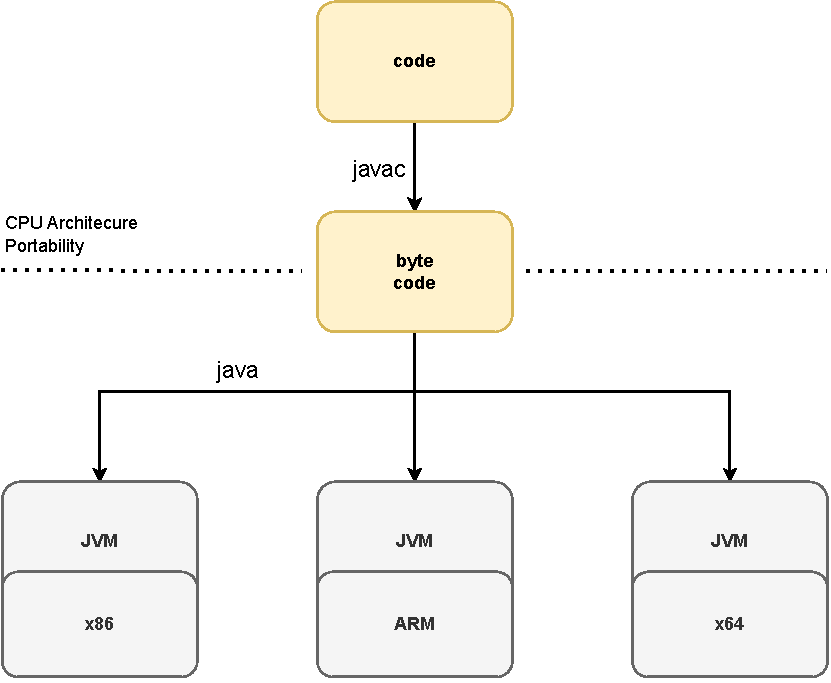
\includegraphics[width=12cm]{images/40_concept/JVM.pdf}
    \caption[Schematische Darstellung des Java-Kompilierungs- und Ausführungsprozesses]{Schematische Darstellung des Java-Kompilierungs- und Ausführungsprozesses~\parencite[vgl.][]{Lindholm2023JavaVM}.}
    \label{fig:JVMAOT}
\end{figure}
Die Bedeutung dieser Aussage wird durch eine Definition im JVM-Standard \citetitle{Lindholm2023JavaVM}~\parencite[vgl.][]{Lindholm2023JavaVM} verdeutlicht, die die essentiellen Prinzipien der Plattformunabhängigkeit von Programmcode betont:
 
 \begin{spar}
 \textit{The Java Virtual Machine knows nothing of the Java programming language, only of a particular binary format, the class file format. A class file contains Java Virtual Machine instructions (or bytecodes) and a symbol table, as well as other ancillary information. \parencite{Lindholm2023JavaVM}}
 \end{spar}

Innerhalb der Ausführungsumgebung der \ac{JVM} erfolgt die Verarbeitung des generierten Bytecodes. Dies wird in Abbildung \ref{fig:JVMEXEC} veranschaulicht.
\newline
 \begin{figure}[H]
    \centering
    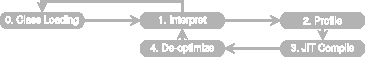
\includegraphics[width=12cm]{images/40_concept/path127.pdf}
    \caption[Darstellung des Ausführungszyklus innerhalb der \ac{JVM}]{Darstellung des Ausführungszyklus innerhalb der \ac{JVM}~\parencite[vgl.][]{9678709}{}{}.}
    \label{fig:JVMEXEC}
\end{figure}
Diese Verarbeitung beinhaltet das Laden der Class-Files, welche den Bytecode beinhalten, und dessen Transformation in Machine-Code. Ein sogenannter ''Interpreter'' ist für die Interpretation der Byte-Code-Instructions zuständig und wandelt diese in ausführbare Machine-Code-Instructions um~\parencite{Lindholm2023JavaVM}.

Die \ac{JVM} implementiert einen Optimierungsprozess während der Konvertierung des Bytecodes durch den \ac{JIT}-Compiler. Dazu nutzt die \ac{JVM} ein Verfahren namens \textit{Profiling}, um zu identifizieren, welche Teile des Codes beispielweise häufig interpretiert werden. Die Relevanz dieses Profiling-Mechanismus wird in \textit{\citetitle{9678709}} erläutert:

\begin{spar}
\textit{The JIT compiler cannot perform sophisticated code analysis and code optimization} when JVM does not have a complete picture of a Java method. JVM thus accumulates method execution counters and collects various method profiling data during interpretation.~\parencite[][]{9678709}{}{}
\end{spar}

Basierend auf dem Profiling-Prozess wird der sogenannte \textit{''Hot-Code''} direkt in nativen Code kompiliert und optimiert. Diese Vorgehensweise eliminiert die Notwendigkeit für eine wiederholte Übersetzung von Bytecode-Instructions in Machine-Code-Instructions durch den Interpreter, indem sie direkten Zugriff auf den durch den JIT-Compiler optimierten Machine-Code ermöglicht~\parencite{Lindholm2023JavaVM}.


\subsection{Limitierungen von Just-in-time im Kontext JRE}

In der Domäne der \ac{JVM} basierten Anwendungen manifestieren sich spezifische Herausforderungen. Initialisierungszeit und Speicherplatzbedarf sind mitunter Probleme, mit denen man konfrontiert ist. Aus diesen Herausforderungen forumliert sich die Hypothese aus Kapitel \ref{subsec:hypothesis:ressource}. Traditionelle Anwendungssysteme charakterisieren sich durch erhebliche Latenzen bei der Initialisierung. Dies untermauert auch das Werk \textit{\citetitle{9678709}}. Dieses ergründet diese durchaus langen Latenzzeiten mit folgender Aussage:

\begin{spar}
    \textit{Largescale Java applications usually have tens of thousands of Java classes or even more, which are packaged into thousands of JAR files. In practice, it can take minutes for those applications to start up before they are online and begin to process user requests.~\parencite[][]{9678709}{}{}}
\end{spar}

Demgegenüber steht die Anforderung, dass Anwendungen, welche den Prinzipien \newline Cloud-nativer Architekturen folgen, signifikant reduzierte Startzeiten aufweisen, ein markanter Kontrast zu den vormals üblichen, durchaus längeren Zeiträumen. Obwohl diese reduzierte Initialisierungszeit für eine Vielzahl von Anwendungsfällen als adäquat betrachtet wird, ergibt sich für Cloud-Architekturen, die eine quasi-instantane Verfügbarkeit erfordern, eine nicht zu vernachlässigende Problematik~\parencite[vgl.][]{12Factor}. 

 
 \subsection{Definition von Ahead-of-time und Anwendung mit GraalVM}
 Im Vergleich zu \ac{JIT} ist \ac{AOT} ein vollkommen anderer Ansatz. Die \acl{AOT} übersetzt Hochsprachencode in Machine-Code bevor das Programm ausgeführt wird, also während der Kompilierzeit. Dies steht im Kontrast zur \acl{JIT}, die Code erst während der Laufzeit kompiliert. AOT bereitet den Code so auf, dass er direkt ausführbar ist. 
 Spricht man nun über den Kontext in Java, bietet die GraalVM \parencite[vgl.][]{graalvm2023} eine Alternative zu vorhandenen JDKs. Dieser GraalVM Standard ist eine Ausprägung der OpenJDK und teil des OpenJDK's Graal Projektes. Dieses Projekt verfolgt grundsätzlich folgendes Ziel:

 \begin{spar}
 \textit{[...]designed to accelerate the execution of applications written in Java and other JVM languages.~\parencite{graalvm2023}}
 \end{spar}

 Als OpenJDK-Alternative soll dieser Ansatz laut \citetitle{graalvm2023}~\parencite[vgl.][]{graalvm2023} eine Steigerung der Effizienz sowie Leistung bringen. Der Graal-Compiler, welcher nun für die Kompilierung von Applikationscode zuständig ist, bietet zwei Betriebsmodi: vorab kompilierter Maschinencode \textbf{\textit{(''libgraal'')}} oder dynamisch ausgeführter Java-Bytecode \textbf{\textit{(''jargraal'')}}. Der GraalVM Native-Image-Builder, welcher eine direkte Kompilierung von Java-Anwendungen in Maschinencode durchführt, ist für ersteren Betriebsmodi zuständig. Das Ergebnis ist ein natives Ausführungsformat, das sämtlichen für die Ausführung notwendigen Maschinencode enthält. Dieser Maschinencode muss nun nicht mehr in einer \ac{JVM} interpretiert und in Maschinencode umgewandelt werden, da dieser Vorgang bereits zu Kompilierzeit erfolgt.

\subsection{Evaluierung der \acl{AOT}}
Die \ac{AOT}-Kompilierung in Java bietet eine Reihe von Vorteilen aber bringt auch Herausforderungen mit sich. Diese werden im folgenden Abschnitt aufgezeigt.

 \textbf{Vorteile der \acl{AOT}}
\begin{enumerate}
    \item \textbf{Verbesserung der Laufzeitperformance:} \ac{AOT}-Kompilierung kann die Startzeit von Java-Anwendungen erheblich reduzieren, indem die Interpretation und Optimierung zur Laufzeit nicht mehr notwendig ist~\parencite[vgl.][]{9678709}.

     \item \textbf{Minimierung der ''Warm-Up''-Phase:} Mit \ac{AOT}-Artefakten erreicht man unmittelbar nach dem Start der Applikation die maximale Leistungsfähigkeit, ohne eine sogenannte ''Warm-Up''-Phase~\parencite[vgl.][]{9678709}. 
\end{enumerate}
 \textbf{Nachteile der \acl{AOT}-Kompilierung}
\begin{enumerate}
    \item \textbf{Verlust der Plattformunabhängigkeit:} Ein wesentlicher Nachteil von \ac{AOT}-Kompilierung ist der Verlust der Plattformunabhängigkeit. Im Unterschied zu \ac{JIT}-Compilern, die plattformübergreifenden Bytecode in Maschinencode umwandeln, produzieren \ac{AOT}-Compiler direkt plattformspezifischen Code. 
    
    \item \textbf{Längere Kompilierungszeiten:} Die Erstellung von \ac{AOT}-Artefakten kann länger dauern als die Erstellung mit \ac{JIT}-Kompilierung, da die gesamte Anwendung im Voraus kompiliert wird. Auf diesen Nachteil wird unter anderem auch in Kapitel \ref{chap:evaluation} eingegangen.

\end{enumerate}

\subsection{Integration in den Web-Crawling Kontext}

Die Implementierung der diskutierten Technologie im Rahmen von Web-Crawling Prozessen adressiert potenziell die Herausforderungen, die in Kapitel \ref{sec:problem} dargelegt wurden. Für Web-Crawling-Service-Instanzen ist eine effiziente Verarbeitung großer Datenmengen, wie sie in der Problemstellung beschrieben wird, essenziell. Dieser Prozess sollte möglichst ressourcenschonend sein. So ist dies eine vielversprechende Technik, um einige Probleme in diesem Kontext zu lösen.

Referenziert auf die Hypothese \ref{subsec:hypothesis:ressource} könnten in diesem Zusammenhang insbesondere die optimierten Startzeiten zu einer erheblichen Verbesserung führen.

Der Web-Crawling Prototyp wird nun auf diese Weise optimiert, um eine gezielte Aussage treffen zu können. Diese Implementierung ist in Kapitel \ref{sec:aotoptimizing} beschrieben.
\chapterend        % concept/design of solution
%%%%%%%%%%%%%%%%%%%%%%%%%%%%%%%%%%%%%%%%%%%%%%%%%%%%%%%%%%%%%%%%%%%%%%%%%%%%%
\chapter{Implementation}
\label{chap:implementation}
%%%%%%%%%%%%%%%%%%%%%%%%%%%%%%%%%%%%%%%%%%%%%%%%%%%%%%%%%%%%%%%%%%%%%%%%%%%%%
\chapterstart

\section{Implementierung der Microservices} \label{sec:impl}
Kapitel \ref{sec:impl} fokussiert sich auf die Implementierung von Microservices, ein Kernaspekt für die Entwicklung skalierbarer Anwendungsarchitekturen. Abschnitt \ref{subsec:techstack} erläutert die Auswahl des Technologiestacks und bietet Einblicke in die Entscheidungsgrundlagen für die verwendeten Technologien. Der Prozess zur Entwicklung der Microservices wird in Abschnitt \ref{subsec:entwmicro} dargestellt, inklusive der methodischen Schritte zur Erstellung der Services. Abschnitt \ref{subsec:eventbas} diskutiert die Implementierung eventbasierter Kommunikation zwischen den Microservices.
\subsection{Auswahl und Begründung des Technologiestacks} \label{subsec:techstack}
Für die Entwicklung der Microservices wurde das Spring Framework in Kombination mit Java eingesetzt. Java, eine objektorientierte Programmiersprache, bildet die Grundlage für die Erstellung von stabilen und wartbaren Anwendungen. Die Wahl von Java stützt sich zudem auf dessen weitreichende Verbreitung, was für die Evaluierung der beiden Hypothesen relevant ist. Diese Entscheidung basiert auf den Erkenntnissen aus Umfragen, beispielweise \citetitle{pyp}~\parencite[vgl.][]{pyp}, das die Verbreitung von Programmiersprachen in der Softwareentwicklung thematisiert. Auch das Buch \citetitle{vitale}~\parencite[vgl.][]{vitale} nennt Programmiersprachen für Cloud-native Applikationen. Vor diesem Hintergrund wurde Java als objektorientierte Programmiersprache für das Projekt herangezogen. 

Das Spring-Framework spielt in diesem Werk eine zentrale Rolle bei der Entwicklung von Microservices mit Java, indem es wesentliche Funktionen für Dependency-Injection bietet. Insbesondere erleichtert es die Integration mit Technologien wie Datenbankverbindungen und die Anbindung an Message-Broker. Spring Boot, eine Erweiterung des Spring-Frameworks, vereinfacht zusätzlich die Softwareentwicklung in diesem Bereich. Die Umsetzung jedes Services erfolgt als Java/Spring Microservice, gemäß der in dieser Arbeit vorgenommenen Implementierungsentscheidung. Es ist jedoch zu beachten, dass Microservices, abhängig von der Architekturentscheidung, auch auf anderen Technologiestacks basieren können, sofern sie die definierten externen Schnittstellen beibehalten. Diese Flexibilität wurde bereits in Kapitel \ref{chap:concept} diskutiert.

\subsection{Entwicklungsprozess der Microservices} \label{subsec:entwmicro}
Zur Erstellung jedes Microservices dient Backstage, ein von Spotify entwickeltes Scaffolding Tool. Dieses Tool automatisiert den Erstellungsprozess von Projekten, indem es auf ein vordefiniertes Template\footnote{\url{https://github.com/avollmaier/templates}}, bekannt als Skeleton, zugreift und daraus eine Applikation generiert. Der Konfigurationsprozess für die Generierung sowie das Skeleton müssen nur einmal definiert werden, können jedoch für die Produktion weiterer Microservices beliebig oft repliziert werden. Das verwendete Skeleton bietet eine standardisierte Struktur, die die Einhaltung von Best Practices und konsistenten Entwicklungsstandards innerhalb der Microservice-Architektur sicherstellt.

Die Nutzung des Build-Tools ''Gradle'' im Projekt legt eine spezifische Projektstruktur fest, die eingehalten werden muss. Gradle strukturiert Projekte in einer Weise, die eine klare Trennung zwischen Produktionscode und Testcode fördert. Diese Strukturierung erleichtert die Build-Automatisierung und verbessert die Übersichtlichkeit des Projekts~\parencite[vgl.][]{gradledocs}{}. Das \lstinline{src}-Paket, das den Quellcode enthält, wird üblicherweise in Unterordner wie \lstinline{main} für den Anwendungscode und \lstinline{test} für den Testcode unterteilt. Die Verwendung von JUnit für die Testfälle im \lstinline{test}-Paket ermöglicht  eine standardisierte und weitverbreitete Methode für Unit-Tests in Java-Projekten, was die Qualitätssicherung der Software unterstützt.
\begin{figure}[H]
    \begin{center}
        \begin{forest}
            for tree={
            font=\ttfamily,
            grow'=0,
            child anchor=west,
            parent anchor=south,
            anchor=west,
            calign=first,
            edge path={
            \noexpand\path [draw, \forestoption{edge}]
            (!u.south west) +(7.5pt,0) |- node[fill,inner sep=1.25pt] {} (.child anchor)\forestoption{edge label};
            },
            before typesetting nodes={
            if n=1
            {insert before={[,phantom]}}
            {}
            },
            fit=band,
            before computing xy={l=15pt},
            }
            [<project-root>
            [src
            [main
            [java
            [resources]
            ]
            ]
            [test
            [java
            [resources]
            ]
            ]
            ]
            ]
        \end{forest}
    \end{center}
    \caption[Vorgegebene Standard Projektstruktur von Gradle]{Vorgegebene Standard Projektstruktur von Gradle~\parencite[vgl.][]{gradledocs}{}.}
\end{figure}

Im Rahmen der \ac{DDD} Strategie, welche für den Prototypen angewandt wird, erfolgt die Entwicklung der Microservices mit dem Ziel, Infrastruktur, Domäne und Applikationsschicht voneinander zu isolieren. Spring unterstützt diesen Prozess durch Bereitstellung spezifischer Tools für jede Schicht. Das Paket \lstinline{org.springframework.boot:spring-boot-starter-web} ermöglicht die Erstellung von Web-Anwendungen, die für die Handhabung von REST-Anfragen im Manager Service verwendet werden. Das Paket \lstinline{org.springframework.boot:spring-boot-starter-data-mongodb} dient zur Anbindung einer MongoDB an den Manager-Service. Diese Werkzeuge fördern die Umsetzung von \ac{DDD}, indem sie eine effiziente Strukturierung und Entkopplung der Systemkomponenten ermöglichen.

\begin{figure}[H]
    \centering
    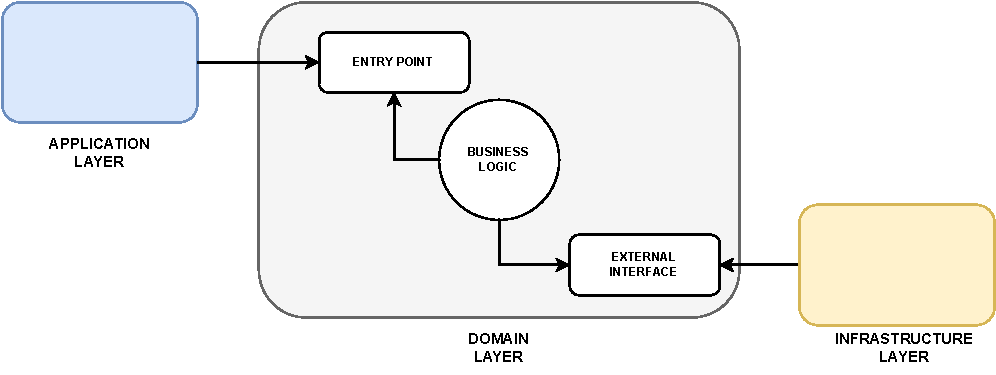
\includegraphics[width=14cm]{images/60_implementation/DDD.drawio.pdf}
    \caption[Darstellung des Domain-Driven-Designkonzepts]{Darstellung des Domain-Driven-Designkonzepts samt Visualisierung der Application-, Domain- und Infrastructure-Layer.}
    \label{fig:DDD}
\end{figure}
\newpage
Die vorliegende Grafik zeigt eine Projektstruktur, die sich an den Prinzipien des \ac{DDD} orientiert. Diese Struktur wird als Leitfaden für alle Implementierungen der Microservices genutzt, wobei die Abhängigkeiten zwischen den Paketen gemäß der in Abbildung \ref{fig:DDD} definierten Beziehungen festgelegt und implementiert werden. Innerhalb dieser Struktur sind verschiedene Pakete zu finden:

\begin{itemize}
    \item \textbf{config}: Dieses Paket enthält Konfigurationsdateien und -klassen, die für das Gesamtprojekt relevant sind, wie beispielsweise Datenbankverbindungen oder Sicherheitseinstellungen.
    
    \item \textbf{domain}: Der Kern des DDD-Ansatzes, das Domain-Paket, beherbergt die Geschäftslogik und ist unterteilt in:
    \begin{itemize}
        \item \textbf{exception}: Klassen, die spezifische Ausnahmen und Fehlerbehandlungen für die Domäne definieren.
        \item \textbf{model}: Enthält die Domänenmodelle oder Entitäten.
        \item \textbf{repository}: Interfaces, die den Zugriff auf die Datenquelle abstrahieren, was für die Anbindung an Datenbanken im Sinne des Repository-Musters steht.
        \item \textbf{service}: Dienste, die Geschäftslogik-Operationen ausführen, indem sie auf Modelle und Repositories zugreifen.
    \end{itemize}
    
    \item \textbf{web}: Dieses Paket ist für die Präsentations- und Interaktionsschicht zuständig, welche die DDD-Schichten ergänzt:
    \begin{itemize}
        \item \textbf{controller}: Controller-Klassen, die eingehende HTTP-Anfragen verarbeiten und die entsprechenden Dienste der Applikationsschicht aufrufen.
        \item \textbf{dto}: Data-Transfer-Objects, die für die Übertragung von Daten zwischen Prozessen genutzt werden, oft als Teil des Controllers, um Daten in einem netzwerkfähigen Format zu senden oder zu empfangen.
    \end{itemize}
    
    \item \textbf{resources}: Ein Paket, das nicht standardmäßig im DDD-Konzept enthalten ist, jedoch häufig Ressourcen wie statische Inhalte, Vorlagen oder Konfigurationsdateien enthält.
\end{itemize}
\begin{figure}[H]
    \begin{center}
        \begin{forest}
            for tree={
            font=\ttfamily,
            grow'=0,
            child anchor=west,
            parent anchor=south,
            anchor=west,
            calign=first,
            edge path={
            \noexpand\path [draw, \forestoption{edge}]
            (!u.south west) +(7.5pt,0) |- node[fill,inner sep=1.25pt] {} (.child anchor)\forestoption{edge label};
            },
            before typesetting nodes={
            if n=1
            {insert before={[,phantom]}}
            {}
            },
            fit=band,
            before computing xy={l=15pt},
            }
            [<package root>
            [config]
            [domain
            [exception]
            [model]
            [repository]
            [service]
            ]
            [web
            [controller]
            [dto]
            ]
            [resources]
            ]
            ]
        \end{forest}
    \end{center}
    \caption{Gewählte Projektstruktur zur Aufteilung der Komponenten nach \acl{DDD}}
\end{figure}
Diese Strukturierung ermöglicht es, die Prinzipien des Domain-Driven-Designs umzusetzen, indem eine klare Trennung zwischen der Geschäftslogik (Domain), der Datenzugriffsschicht (Repositories), der Anwendungsschicht (Services) und der Präsentationsschicht (Web) etabliert wird.
\subsection{Realisierung der eventbasierten Kommunikation zwischen Microservices} \label{subsec:eventbas}
Die Interaktion zwischen den Microservices des Prototypen erfolgt über ein eventbasiertes Modell, implementiert durch das Framework Spring Cloud Stream. Spring Cloud Stream agiert als abstrahierende Schicht, die eine einheitliche Schnittstelle zur Anbindung verschiedener Messaging-Systeme bietet~\parencite[vgl.][]{springcloudstream}. Diese Abstraktion erlaubt es Entwickler/innen, unabhängig vom spezifischen Typ des Messaging-Systems, eine Kommunikation zwischen den Message-Broker und Applikation zu realisieren.

Die Integration von Spring Cloud Stream in einen Microservice des Prototypen erfordert die entsprechende Konfiguration im \lstinline{build.gradle}-File des jeweiligen Projekts. Die Konfiguration der Abhängigkeiten ist in \ref{lst:config1} zu sehen.
\newpage

 \lstinputlisting[language=Java,
                   aboveskip=\floatsep,
                   belowskip=\floatsep,
                   xleftmargin=0cm,         % no extra margins for floats
                   xrightmargin=0cm,        % no extra margins for floats
                   label=lst:config1,   % reference to this listing
                   firstline=22,            % include just a few lines 
                   lastline=26,             % of the given file
                   caption={Konfiguration der notwendigen Spring Cloud Stream Abhängigkeiten.}
                  ]{src/build.gradle}         % the file to be included


Spring Cloud Stream unterstützt eine Vielzahl von Binder-Implementierungen, die für die Integration mit externen Messaging-Systemen konzipiert sind \parencite[vgl.][]{springcloudstream}. Diese Implementierungen umfassen drei zentrale Komponenten: \textit{Destination Binders}, \textit{Destination Bindings} und \textit{Messages}. In den folgenden Abschnitten werden diese erläutert. Zudem wird explizit auf die Konfiguration eingegangen, da diese die essentiellen Bausteine für die Kommunikation der Services sind.
\begin{enumerate}
  \item \textbf{Destination Binder}: Dient als Schnittstelle zwischen den Spring Cloud Stream Anwendungen und dem externen Messaging-System und ist verantwortlich für die Konfiguration der Verbindung.
  \item \textbf{Destination Bindings}: Repräsentieren die Verknüpfung zwischen der Anwendungslogik und den Nachrichtenkanälen des Messaging-Systems.
  \item \textbf{Messages}: Stellen die grundlegende Einheit der Kommunikation dar, die über die definierten Bindings ausgetauscht wird.
\end{enumerate}

\textbf{Konfiguration des Destination Binders}\newline
Die Konfiguration eines externen Messaging-Systems erfordert die spezifische Anpassung des \textit{Destination Binders}, abhängig von den Anforderungen des jeweiligen Systems und den Eigenschaften der Binder. Die Konfiguration dieses Destination Binders erfolgt mit einer Konfiguration (siehe Listing \ref{lst:config2}) des \textit{application.yml} Files im jeweiligen Microservice.
\newpage
 \lstinputlisting[language=Java,
                   aboveskip=\floatsep,
                   belowskip=\floatsep,
                   xleftmargin=0cm,         % no extra margins for floats
                   xrightmargin=0cm,        % no extra margins for floats
                   label=lst:config2,   % reference to this listing
                   firstline=76,            % include just a few lines 
                   lastline=84,             % of the given file
                   caption={[Spring Cloud Stream Konfiguration Destination Binder]Konfiguration des Destination Binders in der application.yml Datei für die Spring Cloud Stream Anbindung.}
                  ]{src/application.yml}         % the file to be included
\textbf{Konfiguration des Destination Bindings}\newline
Als nächsten Schritt muss eine Konfiguration des \textit{Destination Bindings} erfolgen. Dieses Binding verknüpft, wie bereits erwähnt, den Programmcode mit dem Messaging-System. 

Innerhalb der \textit{Destination Bindings} von Spring Cloud Stream wird eine Unterscheidung zwischen zwei Typen getroffen: Ausgehende Bindings, die Nachrichten an ein sogenanntes ''TopicExchange'' im Message-Broker senden (beispielweise \textbf{prioritize-out-0}), und eingehende Bindings, die eingehende Nachrichten mit dem eigentlichen Programmcode verbinden (beispielweise \textbf{prioritize-in-0}). Zu sehen ist diese Konfiguration in Listing \ref{lst:config3}.

\lstinputlisting[language=Java,
                   aboveskip=\floatsep,
                   belowskip=\floatsep,
                   xleftmargin=0cm,         % no extra margins for floats
                   xrightmargin=0cm,        % no extra margins for floats
                   label=lst:config3,   % reference to this listing
                   firstline=66,            % include just a few lines 
                   lastline=76,             % of the given file
                   caption={[Spring Cloud Stream Konfiguration Destination Bindings]Konfiguration des Destination Bindings in der application.yml Datei für die Definition der Input- und Output-Bindings}
                  ]{src/application.yml}         % the file to be included

Die \textit{Destination Bindings} innerhalb von Spring Cloud Stream weisen eine einheitliche Benennungskonvention auf, die eine logische Zuweisung und Identifikation innerhalb der Architektur in der Anwendung unterstützt. Durch die abstrakte Repräsentation der Applikation in Kombination mit dem verwendeten Messaging-Broker, erleichtert Spring Cloud Stream die Verwaltung und Konfiguration dieser Bindings. Die Spezifizierung von \lstinline{<functionName>} in der Konfiguration definiert explizit, welche Komponente der Applikation Nachrichten empfängt oder sendet. Der \lstinline{<index>} hingegen ist in diesem Kontext bei einer einzigen Input-Funktion standardmäßig auf 0 gesetzt.

\begin{itemize}
    \item \textbf{Input-Binding:} \lstinline{<functionName>} + \lstinline{-in-} + \lstinline{<index>}
        \item \textbf{Output-Binding:} \lstinline{<functionName>} + \lstinline{-out-} + \lstinline{<index>}
\end{itemize}
                  
Neben den Input- und Output-Bindings wird in Spring Cloud Stream auch eine \textit{Group}, bekannt als \textit{Consumer Group}, definiert. Diese ermöglicht die Bildung von Gruppen für Subscriber, die am selben Topic teilnehmen. Consumer Groups spielen eine zentrale Rolle bei der Skalierung und Nachrichtenverwaltung in verteilten Systemen, indem sie sicherstellen, dass Nachrichten an Topics nur einmal von einem Mitglied der Gruppe verarbeitet werden. Dieses Konzept wird durch den folgenden Auszug von \citeauthor{springcloudstream}~\parencite[vgl.][]{springcloudstream} verdeutlicht:

\begin{spar}
    \textit{While the publish-subscribe model makes it easy to connect applications through shared topics, the ability to scale up by creating multiple instances of a given application is equally important. When doing so, different instances of an application are placed in a competing consumer relationship, where only one of the instances is expected to handle a given message.~\parencite[][]{springcloudstream}}
\end{spar}

Die Festlegung der \textit{group}-Eigenschaft ist essentiell, wenn mehrere Instanzen eines Microservices bzw. Consumers vorhanden sind. Ohne die Spezifizierung einer \textit{Consumer Group} durch das \textit{group} Property würden alle Instanzen desselben Microservices identische Nachrichten vom Message-Broker empfangen. Die Konfiguration der \textit{group}-Eigenschaft stellt sicher, dass eine Nachricht nur von einer einzigen Instanz innerhalb der spezifizierten Gruppe verarbeitet wird, was der intendierten Funktionsweise entspricht.\newline

\textbf{Konfiguration der Nachricht für Input-/Output-Binding}\newline
Am Ende des Konfigurationsprozesses steht die Definition einer Nachricht, die über den Message-Broker an das entsprechende Topic gesendet wird. In diesem Szenario wird die Nachricht als einfacher Java-Record definiert, wie im Listing \ref{lst:pojo} dargestellt.
\newline
\lstinputlisting[language=Java,
                 xleftmargin=0cm,         % keine zusätzlichen Ränder für Floats
                 xrightmargin=0cm,        % keine zusätzlichen Ränder für Floats
                 label=lst:pojo,   % Referenz auf dieses Listing
                 firstline=7,             % nur einige Zeilen des angegebenen Files einbeziehen
                 lastline=7,              % des angegebenen Files
                 caption={[Java-Record Message Definition]       % Kurzer Titel für das Listingverzeichnis
                           Implementierung eines 
                           Java-Records für eine zu sendende Nachricht über eine StreamBridge Instanz.}
                ]{src/AddressSuppliedMessage.java}

\textbf{Publish einer Nachricht über das Output-Binding}\newline
Anschließend wird die definierte Nachricht mittels der \textit{Stream Bridge} adressiert, einem von Spring Cloud Stream bereitgestellten Bean. Die \textit{Stream Bridge} ermöglicht das Publizieren der vordefinierten Nachricht an den Message-Broker. Das nachfolgende Listing \ref{lst:streambridge} illustriert die Nutzung der injizierten \textit{Stream Bridge} innerhalb einer Methode der Service-Komponente des Manager-Microservices.


\begin{lstlisting}[language=Java, caption=Beispiel einer Methode zur Verarbeitung ausgehender Nachrichten., label={lst:streambridge}]
private final CrawlerManagerRepository crawlerManagerRepository;
private final StreamBridge streamBridge;

public CrawlerManagerService(CrawlerManagerRepository crawlerManagerRepository, StreamBridge streamBridge) {
    this.crawlerManagerRepository = crawlerManagerRepository;
    this.streamBridge = streamBridge;
}
...
private void publishAddressSupplyEvent(Crawler crawler) {
    //UUID zur identifikation der Crawler Konfiguration
    UUID crawlerId = crawler.id();
    
    List<URL> publishAddresses = identifyPublishAdresses(crawler);

    //Erstellen der Message
    var addressSupplyMessage = new AddressSuppliedMessage(crawlerId, publishAddresses);

    //SUPPLY_ADDRESS_OUT = "supplyAddress-out-0"
    var result = streamBridge.send(SUPPLY_ADDRESS_OUT, addressSupplyMessage);
    ...
\end{lstlisting}
\textbf{Subscriben eines Topics über das Input-Binding}\newline
Nach der Konfiguration des Input-Bindings können eingehende Nachrichten durch eine mit \textit{@StreamListener} annotierte Methode (siehe \ref{lst:processIncom}) oder durch die Verwendung von funktionalen Programmiermodellen in Spring Cloud Stream verarbeitet werden. Diese Methoden werden automatisch aufgerufen, wenn eine neue Nachricht im abonnierten Topic erscheint, wodurch die asynchrone Verarbeitung von Ereignissen innerhalb des Microservices ermöglicht wird.
\newpage
\begin{lstlisting}[language=Java, caption=Beispiel einer Methode zur Verarbeitung eingehender Nachrichten., label={lst:processIncom}]
@StreamListener(target = "input")
public void processIncomingMessage(String message) {
    // Logik zur Verarbeitung der Nachricht
}
\end{lstlisting}


Durch den Einsatz von Spring Cloud Stream wird die Verbindung jedes Microservices mit dem Message-Broker ermöglicht, was zu einer  asynchronen Kommunikationsfähigkeit zwischen den Services führt. Diese Architektur ermöglicht es den Microservices, unabhängig voneinander zu operieren und gleichzeitig miteinander zu kommunizieren. Die asynchrone Natur der Kommunikation erleichtert die Skalierung unter hohen Lastbedingungen, indem zusätzliche Instanzen dynamisch hinzugefügt werden können, um die Rechenlast zu verteilen. Diese neuen Instanzen ziehen Nachrichten aus der Queue und verarbeiten sie, wodurch die Gesamtleistung des Systems bei Bedarf flexibel angepasst werden kann. Mit dieser Implementierung wurde unter anderem die Basis für die Evaluierung (Kapitel \ref{sec:comparisonmicroservice}) geschaffen.

\section{Optimierung durch \acl{AOT}} \label{sec:aotoptimizing}
Das Kapitel \ref{sec:aotoptimizing} thematisiert die Optimierung des Prototypen durch \acl{AOT}, welche die Ausführungseffizienz und Startzeit von Anwendungen verbessert. Strategien zur Integration der \acl{AOT} werden in Abschnitt \ref{subsec:trasformationtoaot} vorgestellt. Die Umwandlung des Prototypen in native Images wird in Abschnitt \ref{subsec:integrationaot} beschrieben.
\subsection{Strategien zur Integration der \acl{AOT}} \label{subsec:trasformationtoaot}
Spring Native bietet einen Mechanismus zur Kompilierung von Spring Boot Anwendungen durch GraalVM, mit dem Ziel, jede Spring-Applikation in eine nativ ausführbare GraalVM-Applikation zu transformieren. Dieser Prozess zielt darauf ab, ohne Modifikationen am bestehenden Applikationscode durchführbar zu sein. Dies wird durch die offizielle Dokumentation von \citeauthor{springnative}~\parencite[vgl.][]{springnative}{} unterstrichen.

Die Realisierung dieses Ziels wird durch die Nutzung von Gradle oder Maven-Plugins erleichtert, die alle notwendigen Konfigurationen für die \ac{AOT} der Spring-Klassen durch den GraalVM-Native-Compiler enthalten. Die spezifische Anwendung dieser Plugins und die damit verbundene Konfiguration werden im Kapitel \ref{subsec:integrationaot} detailliert beschrieben.

Um eine Spring Boot Jar in nativen Code zu konvertieren, stehen zwei verschiedene Strategien zur Verfügung. Die erste Methode nutzt das von GraalVM bereitgestellte Command-Line-Tool \lstinline{native-image}, um ein natives Image zu erstellen. Der Befehl hierfür lautet: \lstinline{native-image [options] -jar jarfile [imagename] [options]}. Eine Voraussetzung für die Erstellung eines nativen Images ist das Vorhandensein eines Jar-Archivs oder einer \lstinline{class}-Datei.

Eine alternative Methode zur Erstellung eines \ac{AOT}-Images bietet der Einsatz von Buildpacks, welcher im folgenden Kapitel \ref{subsec:integrationaot} eingehender betrachtet wird, da diese Kompilierungsvariante im Prototypen Anwendung findet.

\subsection{Integration mittels Buildpacks} \label{subsec:integrationaot}
Die Kompilierung einer ausführbaren JAR in ein natives Image mittels Buildpacks\footnote{\url{https://buildpacks.io/}}, insbesondere durch deren Implementierung Paketo\footnote{\url{https://paketo.io/}}, bietet eine standardisierte Methode zur Erstellung von Cloud-nativen Images. Der Buildpacks-Standard zielt darauf ab, die Kompilierung von Cloud-nativen Images zu vereinheitlichen und zu vereinfachen.

Die Kompilierung eines nativen Images mittels Buildpacks erfolgt durch das Command-Line-Tool von Paketo, ''pack''. Dieses Werkzeug ermöglicht eine Erstellung von nativen Images. Der Einsatz von `pack` zur Generierung eines nativen Images wird durch den folgenden Befehl in Listing \ref{lst:bpnative} realisiert.

\begin{lstlisting}[language=bash, caption={Erstellung eines nativen Images mit dem Command-Line-Tool ''pack''.},label={lst:bpnative}]
pack build --builder paketobuildpacks/builder-jammy-tiny \
    --path <path-to-application-jar> \
    --env 'BP_NATIVE_IMAGE=true' \
    service:0.0.1-SNAPSHOT
\end{lstlisting}

Die Ausführung des oben genannten ''pack''-Befehls resultiert in der Erstellung eines nativen Images, das als Container Image exportiert wird. Dieses Image lässt sich in einer Docker-Umgebung mit dem Befehl \lstinline{docker run} starten. Zu sehen ist das in Listing \ref{lst:dockerrun}.

\begin{lstlisting}[language=bash, caption={Starten des nativen Images als Docker-Container.}, label={lst:dockerrun}]
docker run --rm -p 8080:8080 docker.io/library/service:0.0.1-SNAPSHOT
\end{lstlisting}

Um die Erstellung von AOT-Images zu unterstützen, wurde in der \lstinline{build.gradle}-Datei jedes Services ein spezifischer Task mittels Groovy hinzugefügt. Dieser Task ist für das Setzen umgebungsspezifischer Konfigurationen verantwortlich, analog zu den im obigen Befehl dargestellten Einstellungen. Die Integration dieses Schritts in den Buildprozess vereinfacht die Handhabung und Konfiguration der AOT-Kompilierung. Der folgende Groovy-Code (siehe Listing \ref{lst:bootbuildimage}) illustriert die Implementierung eines solchen Tasks im Buildprozess.

\begin{lstlisting}[language=Java, caption={Gradle Task für die Erstellung eines Docker Images mit Paketo Buildpacks.},label={lst:bootbuildimage}]
...
tasks.named('bootBuildImage') {
    builder = 'paketobuildpacks/builder:base'

    if(System.getenv('NATIVE_IMAGE_ENABLED') == 'enabled'){
        println("bootBuildImage is building a native image")
        environment = ['BP_NATIVE_IMAGE': 'true']
    } else {
        environment = ['BP_LIVE_RELOAD_ENABLED': 'true']
    }

    imageName = "${project.name}"

    docker {
        publishRegistry {
            username = project.findProperty("registryUsername")
            password = project.findProperty("registryToken")
            url = project.findProperty("registryUrl")
        }
    }
}
...
\end{lstlisting}
In der gezeigten \lstinline{build.gradle}-Datei (siehe Listing \ref{lst:bootbuildimage}) ist die Konfiguration des Gradle-Tasks (\lstinline{bootBuildImage}) dargestellt, welcher das Paketo Buildpack für die Erstellung eines Docker Images verwendet. Dieser Task wählt basierend auf der Umgebungsvariable \lstinline{NATIVE_IMAGE_ENABLED} zwischen der Erstellung eines nativen Images und der Aktivierung des Live-Reloads. Zudem wird der Image-Name auf den Projektnamen gesetzt und, falls vorhanden, das Docker Image in ein spezifiziertes Docker-Registry hochgeladen.
\chapterend % implementation, prototype
%%%%%%%%%%%%%%%%%%%%%%%%%%%%%%%%%%%%%%%%%%%%%%%%%%%%%%%%%%%%%%%%%%%%%%%%%%%%%
\chapter{Evaluation}
\label{chap:evaluation}
Das Kapitel Evaluation zielt darauf ab, die entwickelten Lösungen und angewandten Methodiken einer umfassenden Bewertung zu unterziehen. Im Fokus steht dabei die Untersuchung, um eine Aussage zu treffen, ob die Hypothesen aus Kapitel \ref{sec:hypothesis} widerlegt oder bestätigt werden können. Diese Evaluierung stützt sich auf definierte Metriken und Benchmarks (siehe Kapitel \ref{sec:metrics}) innerhalb einer konfigurierten Testumgebung (siehe Kapitel \ref{subsec:testenv}), um objektive und reproduzierbare Ergebnisse zu erzielen. Die Ergebnisse werden anschließend im Kapitel \ref{sec:comparison} beurteilt und evaluiert.
%%%%%%%%%%%%%%%%%%%%%%%%%%%%%%%%%%%%%%%%%%%%%%%%%%%%%%%%%%%%%%%%%%%%%%%%%%%%%
\chapterstart

\section{Testumgebung, Testdaten und Metriken} \label{sec:metrics}
Dieses Kapitel befasst sich mit der Definition der Metriken, welche für die Beurteilung der Hypothesen von Relevanz sind. Die Testumgebung dient als Plattform für die Evaluierung und ist so konfiguriert, dass sie reproduzierbare Ergebnisse ermöglicht. In diesem Abschnitt werden die technischen Spezifikationen, die Auswahl der Werkzeuge und die Konfiguration der Umgebung detailliert beschrieben.
\subsection{Testumgebung} \label{subsec:testenv}
Die Evaluierung der Applikationen erfolgt in einer Cloud-nativen Umgebung, für die ein Kubernetes-Cluster als Testplattform dient. Für die Bereitstellung des Kubernetes-Clusters wird das Produkt ''Minikube'' \footnote{\url{https://minikube.sigs.k8s.io/docs/start/}} verwendet. Minikube ermöglicht die Einrichtung eines lokalen Kubernetes-Clusters auf einer einzelnen Maschine und bietet somit eine vereinfachte Plattform für Tests.

Die Host-Maschine für Minikube ist mit einem Intel i7-6700K Prozessor sowie 32 Gigabyte \ac{RAM} ausgestattet und läuft unter einem Debian-basierten Betriebssystem. Diese Konfiguration stellt die Grundlage für die Durchführung der Tests dar und gewährleistet die erforderliche Rechenkapazität sowie Kompatibilität mit der Kubernetes-Infrastruktur.
Durch die Verwendung von Minikube und der spezifizierten Hardware ist es möglich, einheitliche Testbedingungen zu gewährleisten. Dies erleichtert die Bewertung der Applikationsperformance und -skalierbarkeit unter definierten Bedingungen.

Um diese Testumgebung nun in einen testbaren Zustand zu bringen, wird ein Script für das Initialisieren des Minikube-Clusters geschaffen. Dieses Script, welches in Listing \ref{lst:minikubecreate} zu sehen ist, führt mit dem Befehl \lstinline{minikube create} ein Hochfahren des Clusters durch. Nach diesem Schritt werden alle notwendigen Plattform-Services bereitgestellt. Die Definitionen des Deployments dieser Plattform-Services, wie Datenbank und Message-Broker, sind in entsprechenden Konfigurationsdateien hinterlegt.
\newline
\begin{lstlisting}[language=Bash, caption={Script zur Erstellung des Minikube Clusters und dem Deployment der Plattform-Services.},label={lst:minikubecreate}]
#!/bin/sh

echo "Initializing Kubernetes cluster...\n"

minikube start --cpus 8 --memory 16g --driver docker --profile hypercrawler --kubernetes-version=v1.28.3

echo "Deploying platform services..."

kubectl apply -f services

sleep 5

echo "Waiting for MongoDB to be deployed..."

while [ $(kubectl get pod -l db=hypercrawler-mongo | wc -l) -eq 0 ] ; do
  sleep 5
done
...
\end{lstlisting}

\subsection{Datenerfassung und -speicherung}
Für die Erfassung und Speicherung der Metriken aus der Testumgebung wird Prometheus\footnote{\url{https://prometheus.io/}}, ein sogenanntes ''Monitoring-System'', eingesetzt. Prometheus fungiert als zentrales Element für das Monitoring, indem es Metriken von den Applikationen erfasst und persistiert. Diese Metriken werden daraufhin mithilfe eines Scripts abgefragt und in eine CSV-Datei geschrieben. Basierend auf diesen Daten können in weiterer Folge Analysen durchgeführt und Schlüsse gezogen werden. Die Daten werden unter anderem im GitHub-Projekt\footnote{\url{https://github.com/avollmaier/hypercrawler/tree/main/data}} gespeichert, um sie zugänglich zu machen.

Um diese Metriken zu sammeln, sind Konfigurationen in den Applikationen selbst notwendig. Die Applikationen bieten einen spezifischen Endpunkt \lstinline{http://<ip>:<port>/actuator/prometheus} an, der für die Erfassung der Metriken durch Prometheus vorgesehen ist. Dieser Endpunkt wird periodisch (Intervall von 1 Sekunde) von Prometheus abgefragt, wodurch eine fortlaufende und automatisierte Sammlung von Leistungsdaten ermöglicht wird. Die Integration dieses Endpunkts in die Applikationen erfolgt durch Hinzufügen der Abhängigkeit \lstinline{io.micrometer:micrometer-registry-prometheus} in der \lstinline{build.gradle}-Datei jedes Microservices. Dieser Schritt gewährleistet die Bereitstellung der Metriken in einem Format, das von Prometheus gelesen und verarbeitet werden kann. Verwendet wird für diese Anbindung das quelloffene Produkt Micrometer\footnote{\url{https://micrometer.io/}}. Das Ziel von Micrometer kann aus deren Produktdefintion entnommen werden:

\begin{spar}
\textit{Micrometer provides a facade for the most popular observability systems, allowing you to instrument your JVM-based application code without vendor lock-in.~\parencite[][]{micrometer}}
\end{spar}

\subsection{Beschreibung der Testdaten}\label{sec:testdaten}
Die Testdaten für den Crawling-Prozess bestehen aus realen Daten des \ac{WWW}. In \ref{subsec:datacollection} wird die Bedeutung der Diversität in der Größe der Testdaten hervorgehoben. Um die Reproduzierbarkeit der Ergebnisse zu gewährleisten, erfolgte kein Crawling von Live-Daten. Ein solches Vorgehen hätte variierende Ergebnisse zur Folge, bedingt durch Faktoren wie Netzwerklatenz. Daher beruht die Analyse auf statischen Datenquellen. Konkret umfasst sie Daten von Wikipedia, einer Online-Enzyklopädie. Bereitgestellt werden diese durch die Wikimedia Foundation.~\footnote{\url{https://dumps.wikimedia.org}}

Es werden für die Analyse der Hypothese \textit{\nameref{subsec:hypothesis:scalability}} drei statische HTML Auszüge verwendet:
\begin{itemize}
    \item Wikipedia Dump Sprache Tschuwaschisch [\textbf{Sprachkürzel nach ISO-639 CV}] \newline- Auszug vom 07.06 2008 20:30 mit einer Anzahl von 15835 HTML-Seiten \footnote{\url{https://dumps.wikimedia.org/other/static_html_dumps/current/cv/}}
    \item Wikipedia Dump Sprache Biharisch [\textbf{Sprachkürzel nach ISO-639 BH}]\newline- Auszug vom 07.06 2008 12:19 mit einer Anzahl von 4863 HTML-Seiten \footnote{\url{https://dumps.wikimedia.org/other/static_html_dumps/current/bh/}}
 \item Wikipedia Dump Sprache Amharisch [\textbf{Sprachkürzel nach ISO-639 AM}]\newline- Auszug vom 07.06 2008 09:33 mit einer Anzahl von 8618 HTML-Seiten \footnote{\url{https://dumps.wikimedia.org/other/static_html_dumps/current/am/}}
\end{itemize}

Für die Hypothese \textit{\nameref{subsec:hypothesis:ressource}} ist ein Datensatz ausreichend, da an diesem mehrere Tests durchgeführt werden. Verwendet wird hierzu folgender Datensatz:
\begin{itemize}
        \item Wikipedia Dump Sprache Armenisch [\textbf{Sprachkürzel nach ISO-639 HY}]\newline- Auszug vom 07.06 2008 10:46 mit einer Anzahl von 11461 HTML-Seiten \footnote{\url{https://dumps.wikimedia.org/other/static_html_dumps/current/hy/}}
\end{itemize}

Die statischen HTML-Inhalte sind über einen NGINX-Webserver\footnote{\url{https://www.nginx.com/}} zugänglich. Dieser Webserver, ebenso wie sämtliche andere Services, ist Teil der Testumgebung, beschrieben in Kapitel \ref{subsec:testenv}. Das Dockerfile des Docker-Images, dargestellt in Listing \ref{lst:dockernginx}, basiert auf dem offiziellen NGINX-Image. Es definiert auch die Übertragung der statischen Daten in das Image.

\begin{lstlisting}[language=Bash, caption={Dockerfile zur Erstellung des NGINX-Images, versorgt mit Testdaten.},label={lst:dockernginx}]
# Use a lightweight base image
FROM nginx:alpine

# Copy the static website files to the Nginx document root
COPY vo/ /usr/share/nginx/html

\end{lstlisting}
Durch die Ausführung des Befehls \lstinline{docker build -t <imageName> .} werden die Docker-Images, aufgeführt in Tabelle \ref{table:docker_images}, erstellt und sind anschließend verfügbar.

\begin{table}[H]
\centering
\begin{tabular}{|l|l|l|l|l|}
\hline
\textbf{REPOSITORY} & \textbf{TAG} & \textbf{IMAGE ID} & \textbf{CREATED} & \textbf{SIZE} \\ \hline
testdummy-hy & latest & c567e8e5a086 & 16 seconds ago & 255MB \\ \hline
testdummy-cv & latest & 4565997d5061 & 41 seconds ago & 275MB \\ \hline
testdummy-bh & latest & a7519e9f9854 & About a minute ago & 126MB \\ \hline
testdummy-am & latest & 39a4db98377d & About a minute ago & 149MB \\ \hline
\end{tabular}
\caption{Docker Images der Testdaten, bereitgestellt als NGINX-Docker-Image.}
\label{table:docker_images}
\end{table}


\subsection{Metriken zur Messung der Skalierbarkeit der Applikation} \label{}
Um eine Evaluierung der Skalierbarkeit durchzuführen, ist es notwendig die Metriken für die Messung zu definieren. Wie bereits in Abschnitt \ref{sec:method} erwähnt und in der Hypothese in Kapitel \ref{subsec:hypothesis:scalability} definiert, wird in dieser Arbeit die Skalierbarkeit anhand des Crawling-Durchsatzes bestimmt. Der Crawling-Durchsatz eines Webcrawlers, definiert als die Anzahl der in einem bestimmten Zeitraum verarbeiteten Webseiten, kann durch die folgende Formel (siehe \ref{form:durchsatzdefinition}) ausgedrückt werden:

\begin{equation}
    \text{Crawling-Durchsatz} = \frac{\text{Anzahl der verarbeiteten Webseiten}}{\text{Zeitraum}}
    \label{form:durchsatzdefinition}
\end{equation}

wobei der \textbf{Zeitraum} in \textbf{Sekunden} angegeben wird.\newline \newline
Diese Formel wird als Ausgangspunkt für die Evaluierung verwendet. Des Weiteren wird die Gesamtdauer des Crawling-Vorgangs protokolliert. Die Gesamtdauer wird ab dem Zeitpunkt gemessen, wo der Crawling-Prozess gestartet wird. Beendet wird die Messung bei einer vollständigen Untersuchung aller HTML-Seiten. Da die Anzahl der Seiten bekannt ist, kann eine klare Definition des Endes definiert werden. Beide Metriken werden infolgedessen mit einer monolythischen Softwarelösung verglichen.
\subsection{Metriken zur Effizienz von \acl{AOT}}\label{subsec:metrikefficience}
Für die Analyse von \ac{AOT} im Vergleich zu \ac{JIT} werden in der Hypothese \textit{\nameref{subsec:hypothesis:ressource}} folgende Metriken genannt:
\begin{enumerate}
    \item CPU-Nutzung der Applikation
    \item Arbeitsspeicherverbrauch der Applikation
    \item Die Zeit zwischen dem Start der Applikation und der ''Application Readiness'' (Zeitraum bis zu dem Punkt, an dem die Anwendung bereit ist, Anfragen zu bearbeiten)
\end{enumerate}

Die aktuelle CPU-Nutzung wird anhand der Metrik \lstinline{process_cpu_usage} von Prometheus analysiert. 
Für die Analyse des Arbeitsspeicherverbrauchs wird die Metrik \lstinline{jvm_memory_used_bytes} von Prometheus verwendet.

Für die Erfassung der Startzeit wird weder ein Actuator-Endpoint noch Prometheus verwendet. Stattdessen erfolgt die Untersuchung der Application Readiness durch die in Listing \ref{lst:readiness} dargestellte Anpassung. Dabei wird ein sogenannter ''Listener'' registriert, welcher Änderungen im Status der Application Readiness aufzeichnet und anschließend protokolliert. Mit dieser Methode lässt sich die Startzeit der Applikation, definiert als der Zeitraum bis zum Beginn der Annahme von Anfragen, im Bereich von Millisekunden erfassen.

\begin{lstlisting}[language=Java, caption={Code zur Analyse der Application Readiness am Beispiel des Crawler Services.},label={lst:readiness}]
@SpringBootApplication
public class CrawlerApplication {
  private static Long startTimeMillis;

  public static void main(String[] args) {
    startTimeMillis = System.currentTimeMillis();
    SpringApplication.run(CrawlerApplication.class, args);
  }

  @EventListener
  public void onEvent(AvailabilityChangeEvent<ReadinessState> event) {
    if (Objects.requireNonNull(event.getState()) == ReadinessState.ACCEPTING_TRAFFIC) {
      Long readinessMillis = System.currentTimeMillis();
      log.info("Readiness probe completed in {} ms", readinessMillis - startTimeMillis);
    }
  }
}
\end{lstlisting}
\newpage
\section{Evaluierung der Lösungen} \label{sec:comparison}
Das nachfolgende Kapitel hat das Ziel, die erzielten Ergebnisse zu präsentieren, zu evaluieren sowie die formulierten Hypothesen zu verifizieren oder zu falsifizieren. Im Unterkapitel \ref{sec:comparisonmicroservice} erfolgt die Untersuchung der Hypothese bezüglich der Skalierbarkeit (siehe Hypothese \textit{\nameref{subsec:hypothesis:scalability}}). Das Kapitel \ref{sec:comparisonaot} fokussiert sich auf die Überprüfung der Hypothese zur Ressourcennutzung (siehe Hypothese \textit{\nameref{subsec:hypothesis:ressource}}).
\subsection{Evaluierung der Microservice-Architektur hinsichtlich Skalierbarkeit}\label{sec:comparisonmicroservice}
Die Skalierbarkeitsanalyse erfolgte durch die Durchführung von drei Web-Crawling Durchläufen, die jeweils sowohl mit der Microservice als auch mit der Monolithischen Lösung durchgeführt wurden. Dabei wurde der Crawling-Durchsatz und die Gesamtdauer des Crawling-Vorgangs verglichen. Der Crawling-Durchsatz wurde für Zeitrahmen des gesamten Crawling-Prozesses betrachtet. Gemessen wurde ab dem Start des Crawling-Prozesses bis zur Persistierung der letzten HTML-Seite. Diese Zeit wurde in den Tabellen \ref{tab:scalability_analysis_micro} und \ref{tab:scalability_analysis_mono} protokolliert. \newline
Zur Analyse der monolithischen Anwendung wurde ein Java-Projekt erstellt, welches den Crawling-Prozess mithilfe der gleichen Mechanismen durchführt. Dieses Projekt ist im GitHub-Repository des Prototyps einsehbar.\footnote{\url{https://github.com/avollmaier/hypercrawler}}

Um den Zeitpunkt abzufragen, wann der Crawling-Prozess abgeschlossen ist, wurde ein Script erstellt, welches den Zeitpunkt des Starts und des Endes, also den Zeitpunkt ab dem alle Seiten persistiert wurden, misst. Dieses Script liefert die exakten Zeitstempel zurück, mit welchen infolgedessen eine Berechnung des Durchsatzes und der Durchlaufzeit stattfindet. Durch dieses Vorgehen kann die Unsicherheit des Messvorgangs mithilfe der Integration eines automatisierten Prozesses vermieden werden.\newline


\begin{table}[H]
\begin{tabular}{|l|l|l|l|}
\hline
\textbf{Datensatz}                                                      & \textbf{Seitenanzahl} & \textbf{Durchsatz (Seiten/Sekunde)} & \textbf{Durchlaufzeit} \\ \hline
\begin{tabular}[c]{@{}l@{}}Wikipedia Dump\\ Tschuwaschisch\end{tabular} & 15835                       & \textbf{63,09}                                   & \textbf{251 Sekunden}                       \\ \hline
\begin{tabular}[c]{@{}l@{}}Wikipedia Dump\\ Biharisch\end{tabular}      & 4863                             & \textbf{54,64}                                   & \textbf{89 Sekunden}                       \\ \hline
\begin{tabular}[c]{@{}l@{}}Wikipedia Dump\\ Amharisch\end{tabular}      & 8618                             & \textbf{62,45}                                   & \textbf{138 Sekunden}                       \\ \hline
\end{tabular}
\caption{Skalierbarkeitsanalyse des Crawling-Prozesses (Microservice Lösung).}
\label{tab:scalability_analysis_micro}
\end{table}

\begin{table}[H]
\begin{tabular}{|l|l|l|l|}
\hline
\textbf{Datensatz}                                                      & \textbf{Seitenanzahl} & \textbf{Durchsatz (Seiten/Sekunde)} & \textbf{Durchlaufzeit} \\ \hline
\begin{tabular}[c]{@{}l@{}}Wikipedia Dump\\ Tschuwaschisch\end{tabular} & 15835                            & \textbf{50,91}                                   & \textbf{311 Sekunden}                       \\ \hline
\begin{tabular}[c]{@{}l@{}}Wikipedia Dump\\ Biharisch\end{tabular}      & 4863                             & \textbf{51,73}                                   & \textbf{94 Sekunden}                       \\ \hline
\begin{tabular}[c]{@{}l@{}}Wikipedia Dump\\ Amharisch\end{tabular}      & 8618                             & \textbf{50,1}                                   & \textbf{172 Sekunden}                       \\ \hline
\end{tabular}
\caption{Skalierbarkeitsanalyse des Crawling-Prozesses (Monolythische Lösung).}
\label{tab:scalability_analysis_mono}
\end{table}

\textbf{Durchschnittlicher Durchsatz für die Microservice Lösung}\newline
Aus Tabelle \ref{tab:scalability_analysis_micro} werden nun die Durschnittswerte für den Crawling-Durchsatz in der Einheit \textit{Seiten pro Sekunde} berechnet. Diese Berechnung ist in Gleichung \ref{eq:microservice_durchsatz} ersichtlich. 
\begin{equation}
\frac{63,09 + 54,64 + 62,45}{3} = 60,06
\label{eq:microservice_durchsatz}
\end{equation}

\textbf{Durchschnittlicher Durchsatz für die Monolithische Lösung}\newline
Des weiteren wurde der durchschnittliche Durchsatz der Monolythischen Anwendungen mithilfe der Daten aus Tabelle \ref{tab:scalability_analysis_mono} berechnet. Dies ist in Gleichung \ref{eq:monolith_durchsatz} ersichtlich.
\begin{equation}
\frac{50,91 + 51,73 + 50,1}{3} = 50,91
\label{eq:monolith_durchsatz}
\end{equation}

Die Verbesserung in Prozent berechnet sich wie folgt (siehe Gleichung \ref{eq:verbesserung_prozent}):
\begin{equation}
\text{Verbesserung (\%)} = \left( \frac{\text{Neuer Durchsatz} - \text{Alter Durchsatz}}{\text{Alter Durchsatz}} \right) \times 100
\label{eq:verbesserung_prozent}
\end{equation}
\newpage
Setzt man diese Werte in die Formel ein, so erhält man das nachfolgende Ergebnis, wie in Gleichung \ref{eq:verbesserung_prozent_rechnung} ersichtlich:
\begin{equation}
\text{Verbesserung (\%)} = \left( \frac{60,06 - 50,91}{50,91} \right) \times 100 = \left( \frac{9,15}{50,91} \right) \times 100 \approx 17,95\%
\label{eq:verbesserung_prozent_rechnung}
\end{equation}

Die Verbesserung in der Durchsatzleistung beträgt 17,95\%.
Des Weiteren zeigt die Analyse, dass während des Crawling-Durchlaufs (Datensatz Wikipedia Dump Tschuwaschisch Microservice) ein Service nicht in der Lage war, alle Nachrichten zu beantworten, was zu deren Anhäufung führte. Es existiert somit ein Flaschenhals, vor allem bei großen Datensätzen. Wie in der Abbildung \ref{fig:rabbitmq} ersichtlich ist, warten \textbf{3495 Nachrichten} in der Message-Queue. In dieser Situation ist es möglich, den Vorteil zu nutzen, dass eine weitere Instanz dieses Services hochgefahren werden kann, um die Last auf beide Instanzen zu verteilen. So kann ein noch höherer Durchsatz erzeugt werden, da genau bestimmt wird, welche Komponente einen Engpass verursacht. Somit ist eine gezieltere Steuerung als bei einer Monolythischen Lösung möglich. Diese Instanz kann durchaus auch auf einer anderen Maschine laufen, was eine geographische Verteiltheit ermöglicht.
\begin{figure}[H]
    \centering
    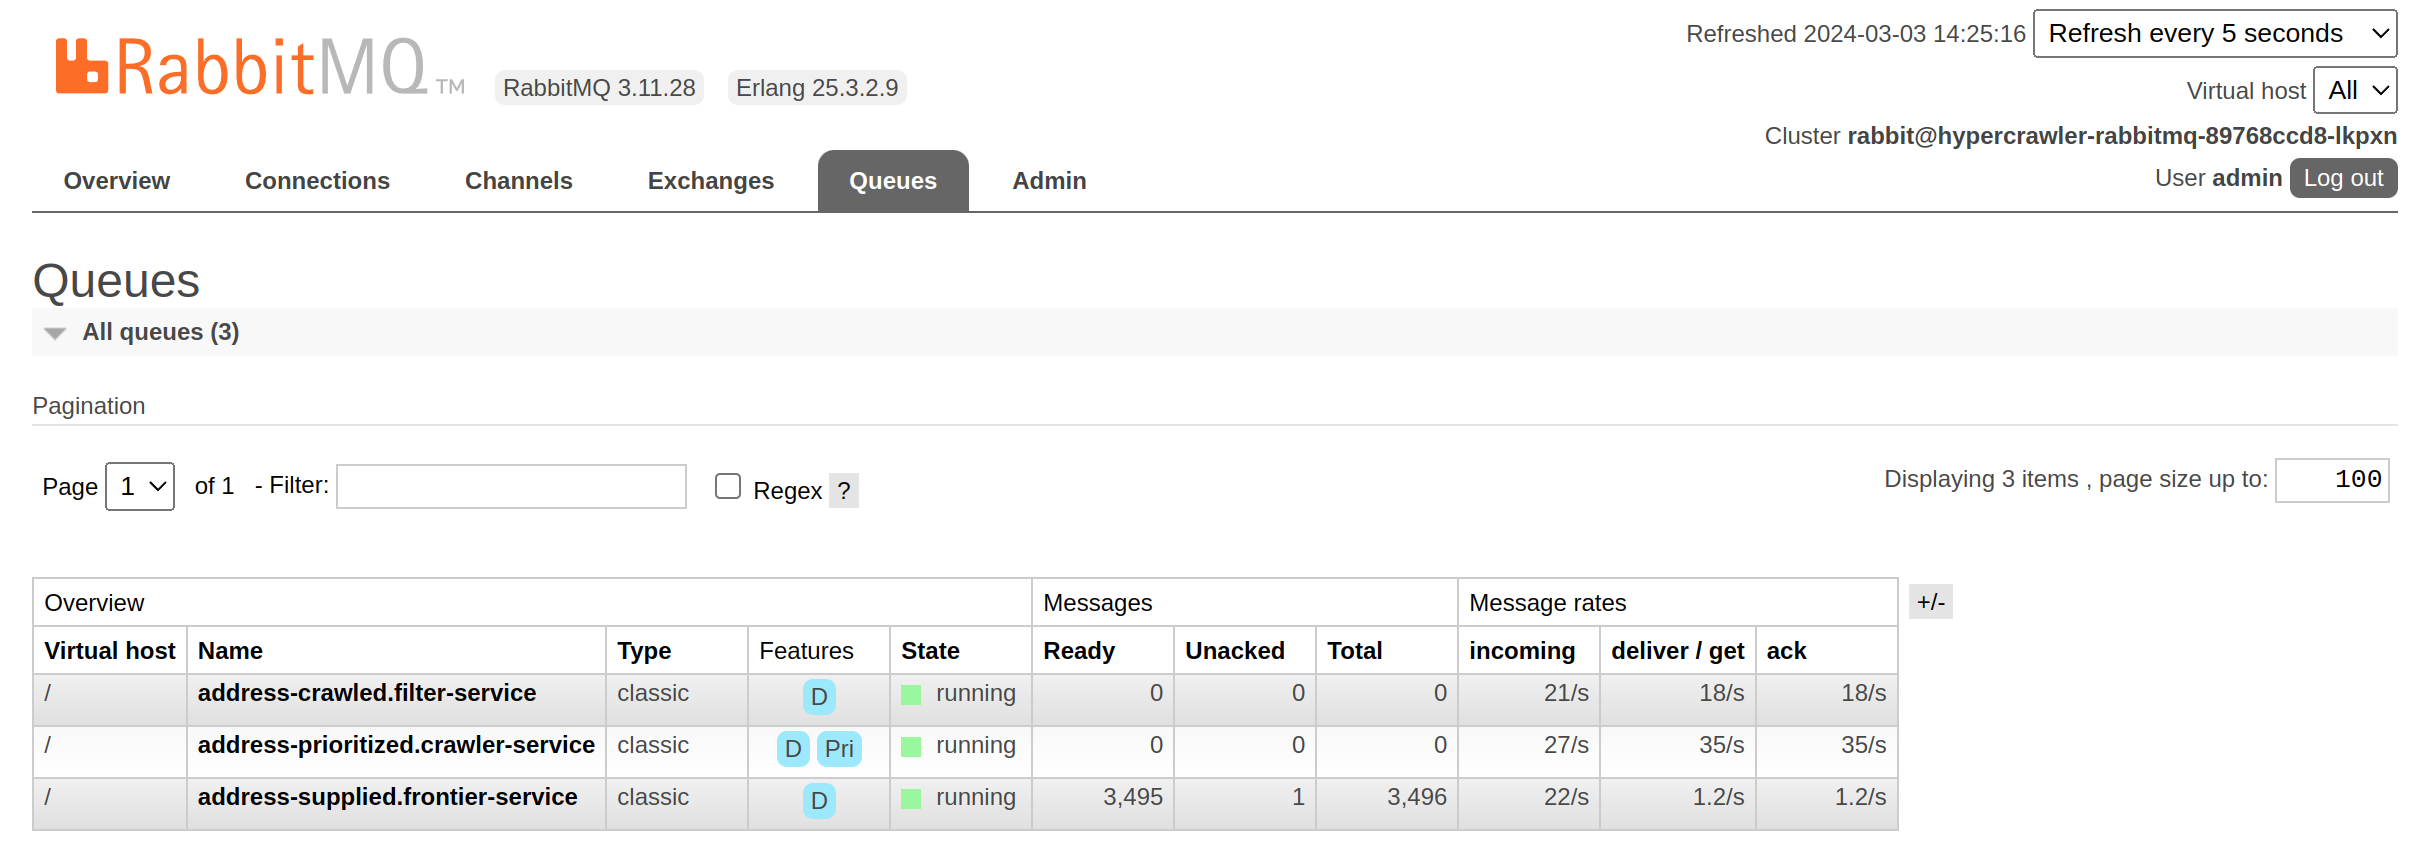
\includegraphics[width=14cm]{images/80_eval/Screenshot from 2024-03-03 14-25-29.png}
    \caption[]{Darstellung der RabbitMQ-Message-Queue mit 3495 unbearbeiteten Nachrichten.}
    \label{fig:rabbitmq}
\end{figure}
\newpage
\subsection{Evaluierung der Verbesserungen der Effizienz durch \acl{AOT}.} \label{sec:comparisonaot}
In diesem Abschnitt wird die CPU-Nutzung und der Speicherverbrauch eines Services untersucht.  Hierzu wird ein Crawling-Vorgang mit beiden Technologien gestartet und danach werden mithilfe von Prometheus die Daten abgefragt. Als Testset wird die statische Webseite von Wikipedia in der Armenischen Sprache verwendet. Damit vergleichbare Werte möglich sind, wurden in beiden Crawling-Prozessen die Werte des \textbf{Crawling Service} abgefragt.  \newline\newline
\textbf{Vergleich der CPU-Nutzung}\newline
Die nachfolgende Abbildung \ref{fig:cpujit} zeigt die CPU-Nutzung in Prozent über den gemessenen Zeitraum. Zu sehen ist die Analyse mit \ac{JIT}-Artefakten. Die Kennwerte für die CPU-Nutzung wurden analysiert wobei folgende Ergebnisse ersichtlich wurden:
\begin{enumerate}
    \item Maximale CPU-Nutzung: 23,5\%
    \item Durchschnittliche CPU-Nutzung: 5,29\%
\end{enumerate}

\begin{figure}[H]
    \centering
    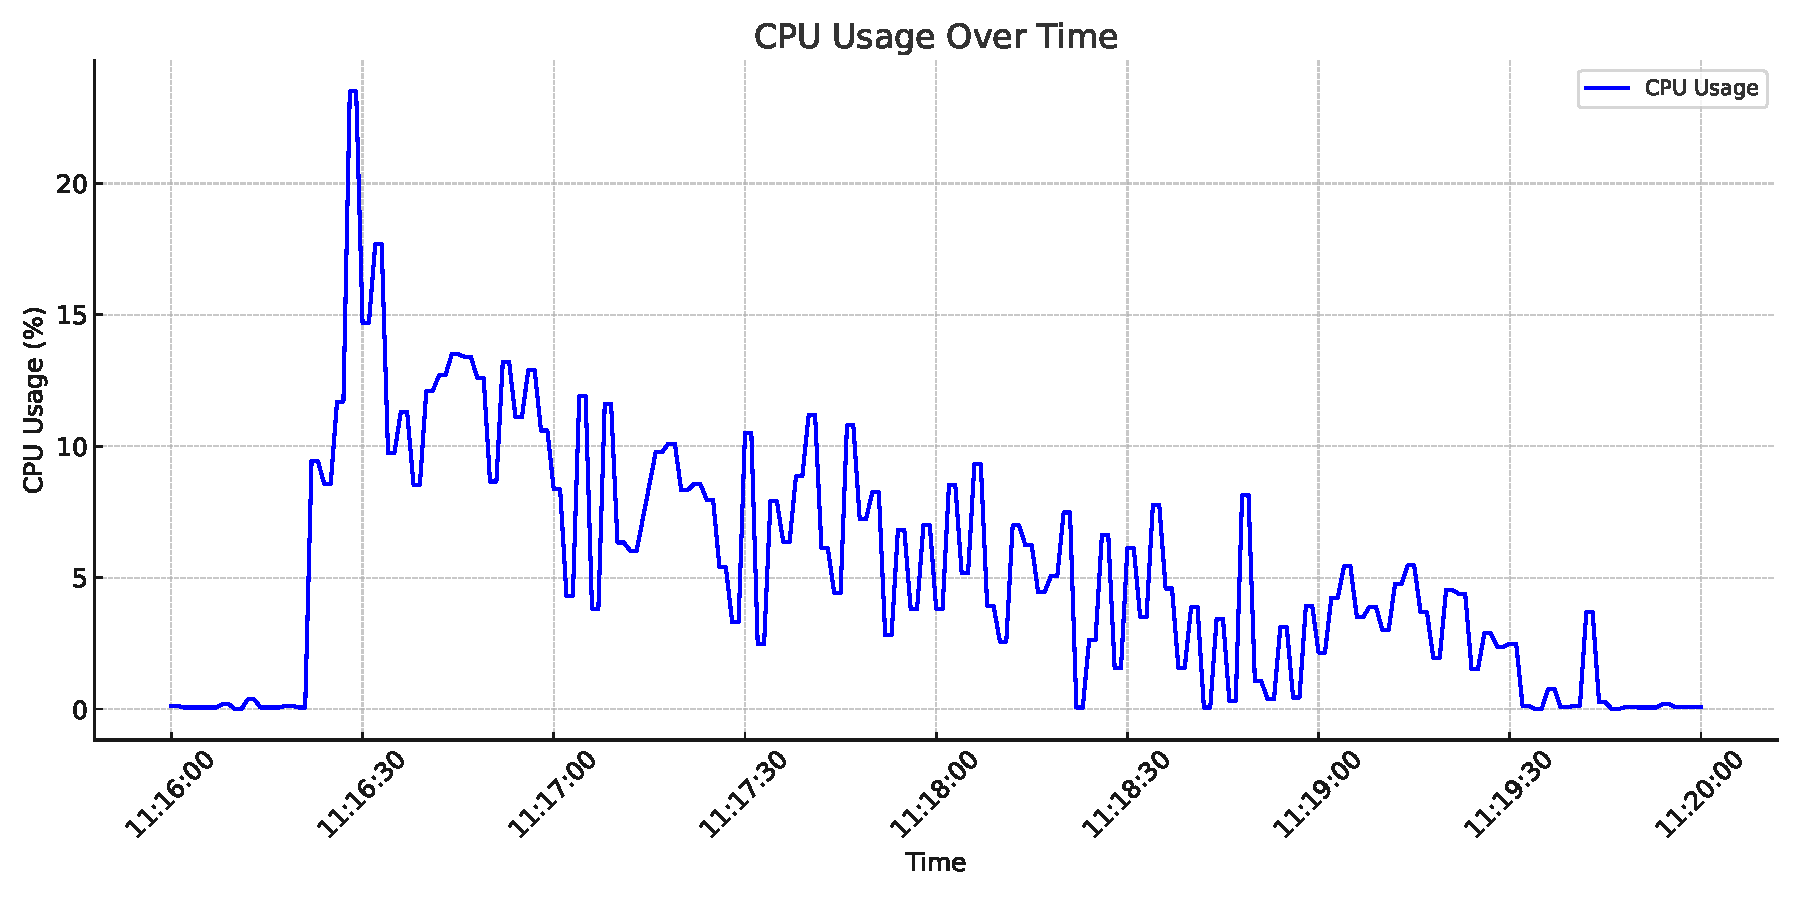
\includegraphics[width=12cm]{images/80_eval/CPU_Usage_Over_Time.pdf}
    \caption[]{Darstellung der CSV-Daten der CPU-Nutzung als Diagramm mit \acl{JIT}.}
    \label{fig:cpujit}
\end{figure}
Die Abbildung \ref{fig:cpuaot} zeigt nun die CPU-Nutzung in Prozent, jedoch mit \ac{AOT}-Artefakten. Aus diesen Daten lassen sich folgende Kennwerte ableiten:
\begin{enumerate}
    \item Maximale CPU-Nutzung: 8,5\%
    \item Durchschnittliche CPU-Nutzung: 2,24\%
\end{enumerate}
\begin{figure}[H]
    \centering
    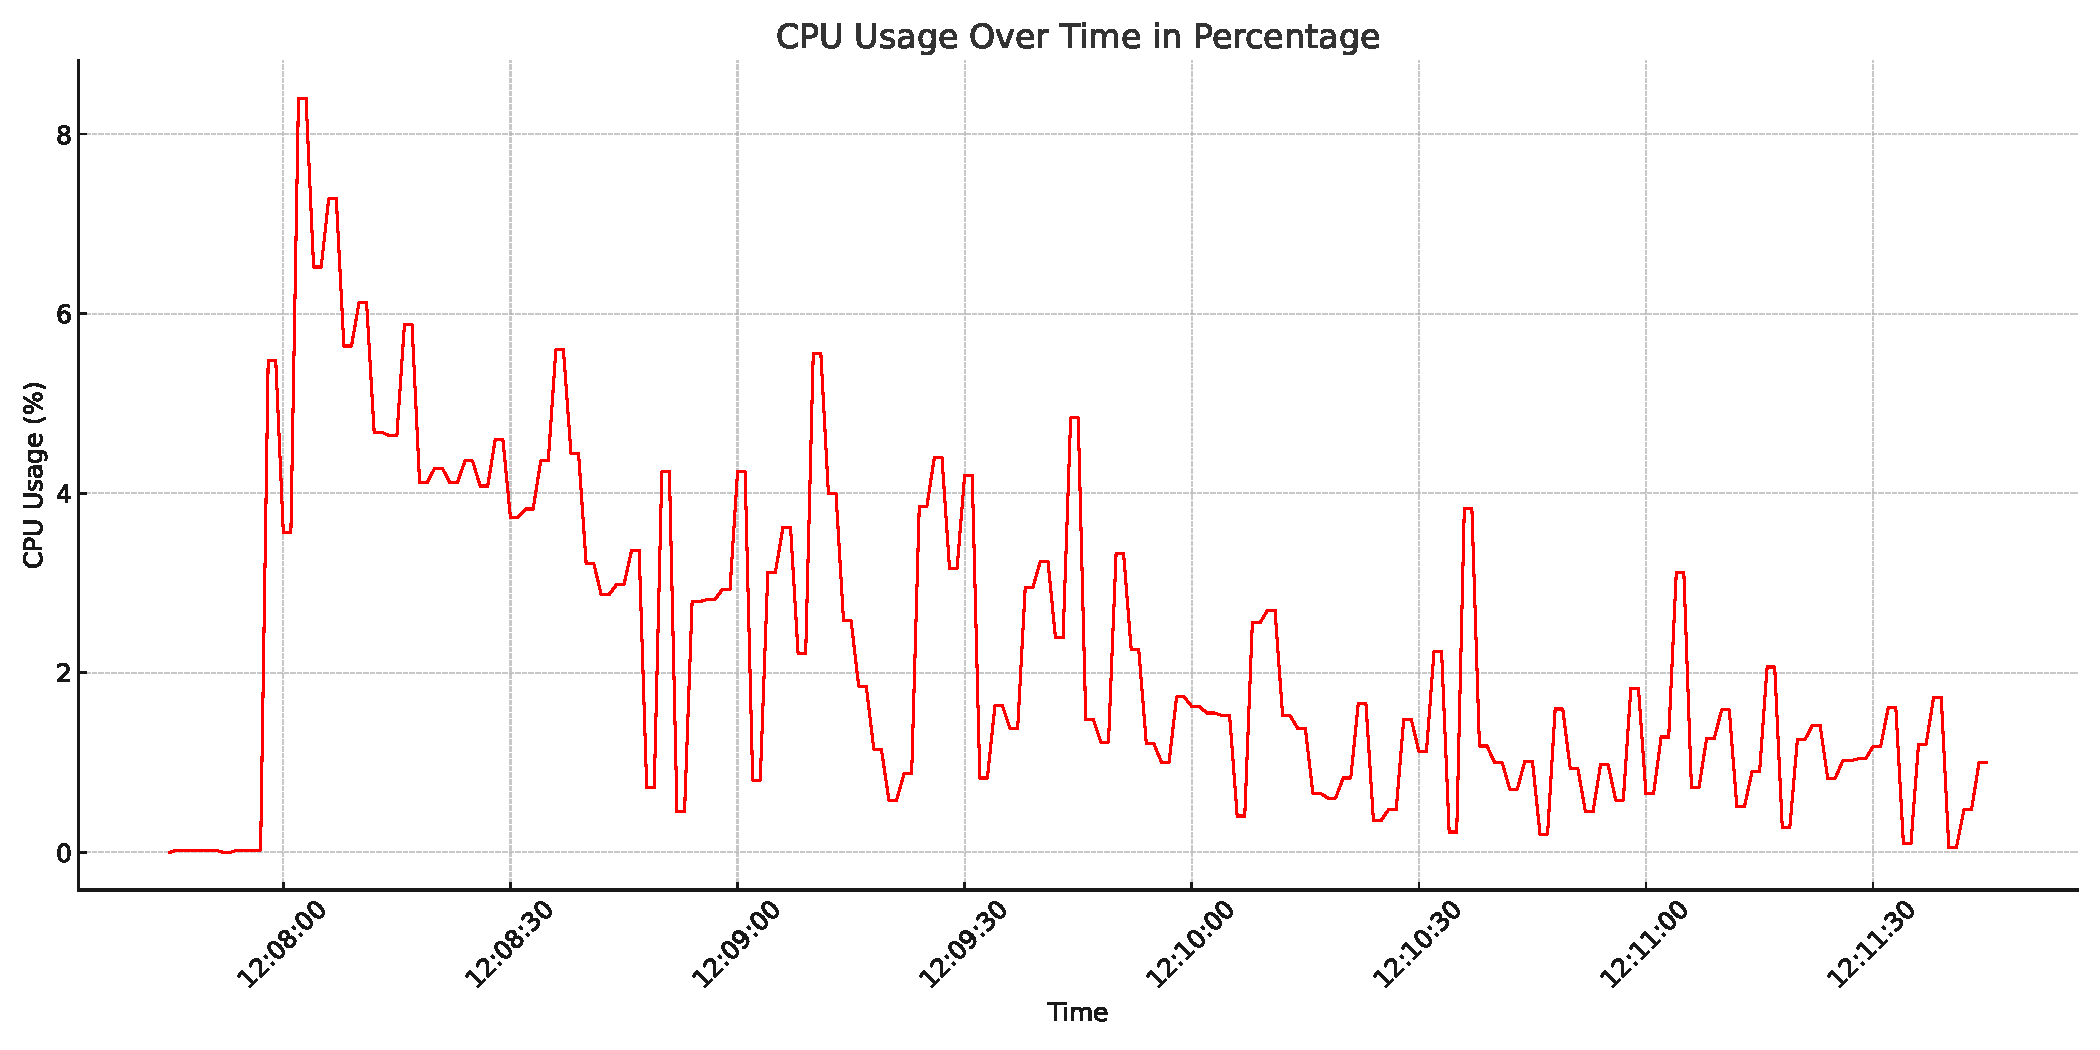
\includegraphics[width=12cm]{images/80_eval/cpu_usage_percentage_simplified_over_time.pdf}
    \caption[]{Darstellung der CSV-Daten der CPU-Nutzung als Diagramm mit \acl{AOT}.}
    \label{fig:cpuaot}
\end{figure}
\textbf{Ergebnisse der Berechnung} \newline
Die \ac{AOT}-Kompilierung zeigt im Vergleich zur \ac{JIT}-Kompilierung eine deutliche Verbesserung in Bezug auf die CPU-Nutzung: \ac{AOT}-Artefakte des Crawler-Service haben in diesem Test eine um 63,8\% geringere maximale CPU-Nutzung als \ac{JIT}-Artefakte des gleichen Serives. Die durchschnittliche CPU-Nutzung der \ac{AOT}-Artefakte ist in diesem Test auch um 57,65\% geringer als mit \ac{JIT}-Artefakte. Diese Berechnung erfolgt anhand der Formel \ref{eq:jitspuc}:
\begin{equation}
\text{Verbesserung (\%)} = \left( \frac{\text{AOT CPU-Nutzung} - \text{JIT CPU-Nutzung}}{\text{JIT CPU-Nutzung}} \right) \times 100    
\label{eq:jitspuc}
\end{equation}

Für die Überprüfung der Hypothese, dass \ac{AOT} eine 20\%ige Verbesserung der CPU-Nutzung gegenüber \ac{JIT} bietet, soll die Differenz im Vergleich zu \ac{JIT} betrachtet werden, da \ac{JIT} der Ausgangspunkt oder der ''vorherige Zustand'' ist und \ac{AOT} der ''verbesserte Zustand''. Diese Formel gilt auch für die Analyse der Speicherauslastung.

Diese Ergebnisse zeigen, dass die \ac{AOT}-Kompilierung in diesem Szenario erheblich effizienter in Bezug auf die CPU-Nutzung ist, als die \ac{JIT}-Kompilierung. Die Hypothese der CPU-Nutzung ist somit verifiziert.\newline \newline
\textbf{Vergleich der Speicher-Nutzung}\newline
Die Abbildung \ref{fig:memjit} zeigt die Nutzung des Arbeitsspeichers über den bestimmten Zeitraum, dargestellt in Megabyte. Die X-Achse der Abbildung stellt die Zeit in regelmäßigen Intervallen dar, während die Y-Achse die Nutzung des Arbeitsspeichers in Megabyte angibt.
Durch die Analyse der Daten wurde festgestellt, dass der durchschnittliche und maximale Nutzungswert wie folgt lautet:
\begin{enumerate}
    \item Maximaler Nutzungswert: 760.75 Megabyte
    \item Durchschnittliche Nutzungswert: 433.70 Megabyte
\end{enumerate}
\begin{figure}[H]
    \centering
    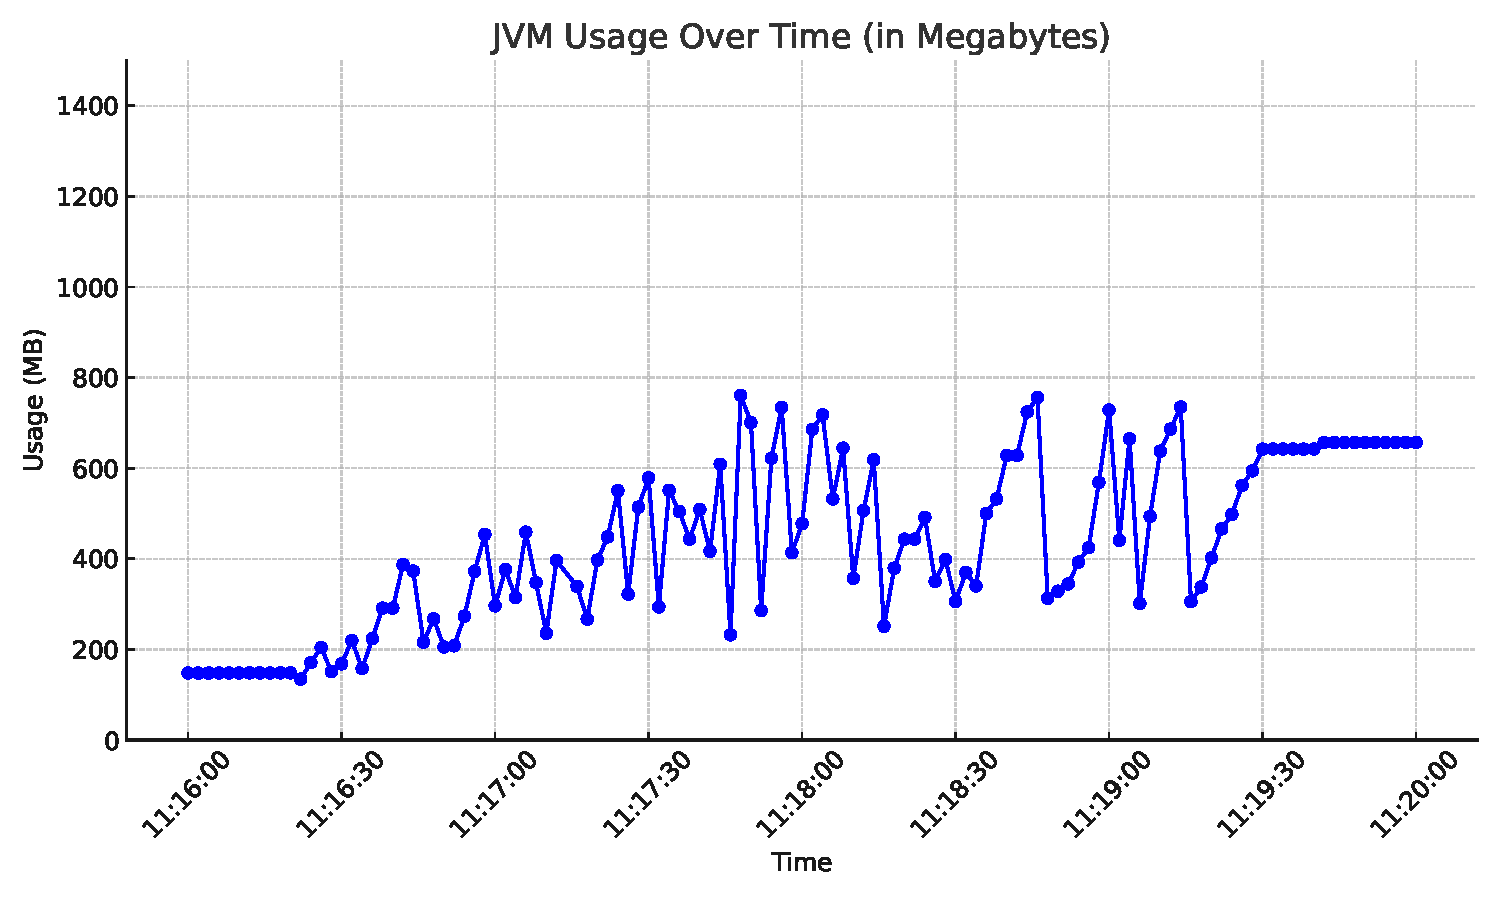
\includegraphics[width=12cm]{images/80_eval/JVM_Usage_Timeseries_MB_1500.pdf}
    \caption[]{Darstellung der CSV-Daten des Speicherverbrauchs als Diagramm mit \acl{JIT}.}
    \label{fig:memjit}
\end{figure}

Außerdem wurde eine Analyse mit \ac{AOT}-Artefakten durchgeführt. Die Abbildung \ref{fig:memaot} zeigt den Verlauf des Speicherverbrauchs. Folgende Kennzahlen lassen sich aus den Daten ableiten:
\begin{enumerate}
    \item Maximaler Nutzungswert: 156,78 Megabyte
    \item Durchschnittliche Nutzungswert: 78.075 Megabyte
\end{enumerate}

\begin{figure}[H]
    \centering
    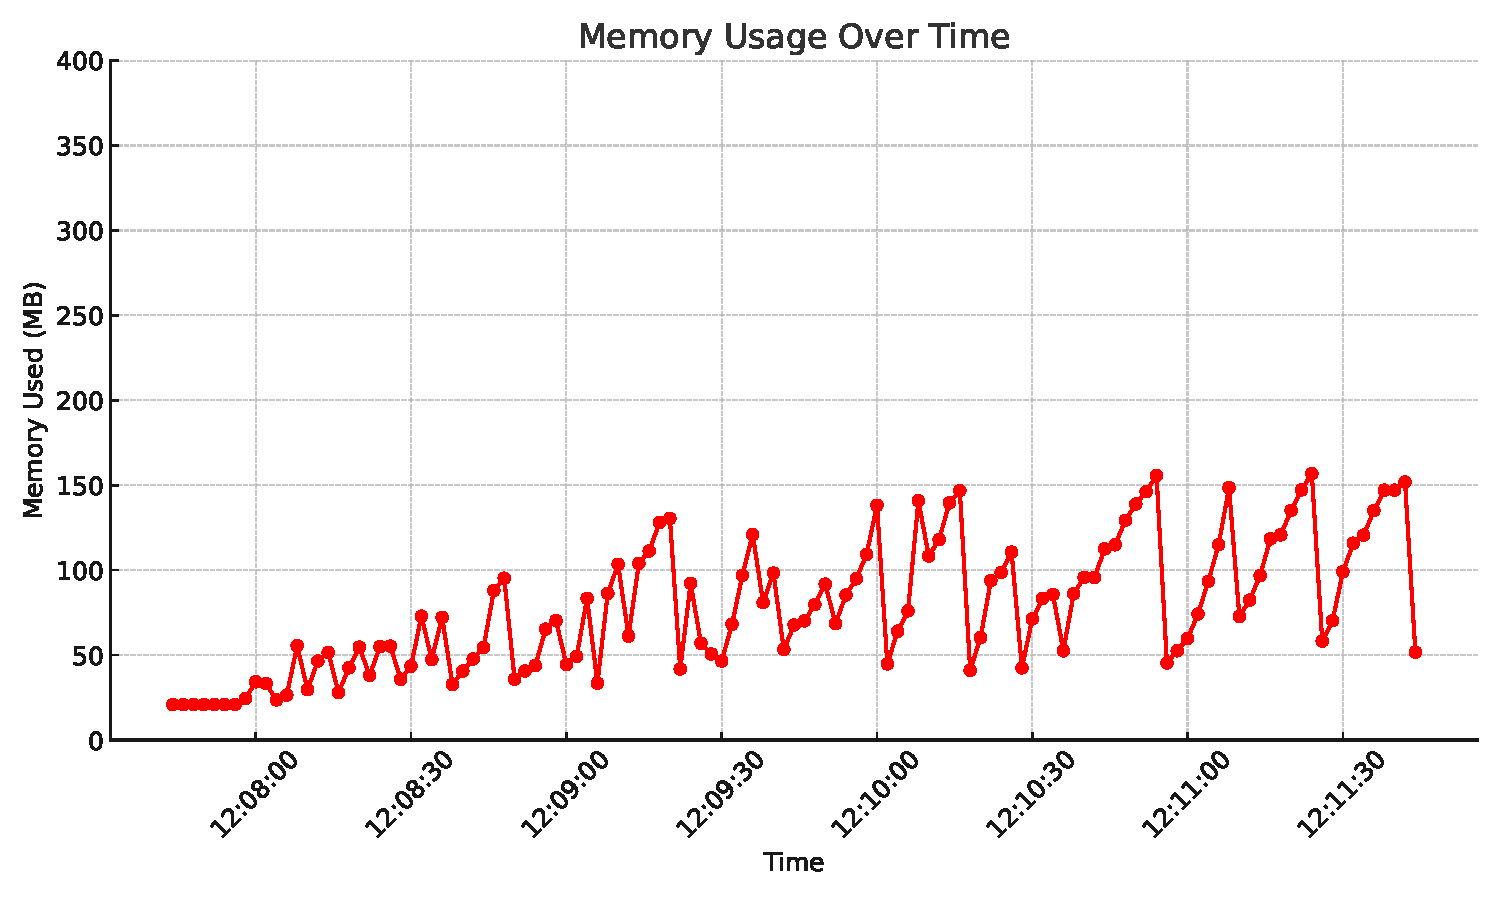
\includegraphics[width=12cm]{images/80_eval/memory_usage_over_time_very_final.pdf}
    \caption[]{Darstellung der CSV-Daten des Speicherverbrauchs als Diagramm mit \acl{AOT}.}
    \label{fig:memaot}
\end{figure}
\textbf{Ergebnisse der Berechnung} \newline
Aus den zuvor aufgestellten Berechnungen lassen sich folgende Verbesserungen ableiten: Für den maximalen Nutzungswert \textbf{79.39\%} und für den durchschnittlichen Nutzungswert \textbf{82.00\%}.

Durch diese Kennzahlen lässt sich ebenfalls eine Optimierung im Bereich des Speicherverbrauchs bestätigen. Folglich ist auch der Aspekt der Hypothese bezüglich der Speichernutzung verifiziert.

\textbf{Vergleich der Startzeit der Anwendungen}\newline
Bei der Durchführung der Lasttests wurden von allen vier Services die Startzeiten analysiert. Einmal mit \ac{AOT} und einmal mit \ac{JIT}. Diese wurden gegenübergestellt und verglichen. Die Startzeiten der \ac{JIT}-Artefakte ist in \ref{tab:startzeitjit} zu sehen.
\begin{table}[H]
\centering
\begin{tabular}{|l|l|l|l|l|}
\hline
\textbf{Anwendung}     & \textbf{Test 1 (ms)} & \textbf{Test 2 (ms)} & \textbf{Test 3 (ms)} & \textbf{Test 4 (ms)} \\ \hline
\multirow{1}{*}{Manager-Service}  & 4526 & 4277 & 4151 & 3916 \\ \hline
\multirow{1}{*}{Frontier-Service}        & 5285 & 5259 & 4567 & 4530 \\ \hline
\multirow{1}{*}{Crawler-Service}         & 4415 & 4587 & 4567 & 4668 \\ \hline
\multirow{1}{*}{Filter-Service}          & 3845 & 3904 & 3818 & 3733 \\ \hline
\end{tabular}
\caption{Startzeit der JIT-Anwendungen bis zur Application Readiness.}
\label{tab:startzeitjit}
\end{table}

Die Artefakte, kompiliert mit \ac{AOT}, wurden den gleichen Tests unterzogen, wie zuvor erwähnt. Die Ergebnisse sind in Tabelle \ref{tab:startzeitaot} protokolliert.
\begin{table}[H]
\centering
\begin{tabular}{|l|l|l|l|l|}
\hline
\textbf{Anwendung}     & \textbf{Test 1 (ms)} & \textbf{Test 2 (ms)} & \textbf{Test 3 (ms)} & \textbf{Test 4 (ms)} \\ \hline
\multirow{1}{*}{Manager-Service}  & 293 & 346 & 558 & 514 \\ \hline
\multirow{1}{*}{Frontier-Service}        & 460 & 277 & 361 & 634 \\ \hline
\multirow{1}{*}{Crawler-Service}         & 298 & 334 & 358 & 712 \\ \hline
\multirow{1}{*}{Filter-Service}          & 461 & 272 & 374 & 379 \\ \hline
\end{tabular}
\caption{Startzeit der AOT-Anwendungen bis zur Application Readiness.}
\label{tab:startzeitaot}
\end{table}
Nach der Analyse wurden die Durchschnittszeiten (nach Formel \ref{equ:startzeiten}) für jeden Service berechnet. Dabei wurden die durchschnittlichen Startzeiten für jede Anwendung unter Verwendung unterschiedlicher Technologien ermittelt. Die Ergebnisse sind in Tabelle \ref{table:druch} protokolliert.
\begin{equation}
\text{Durchschnitt} = \frac{\sum \text{Startzeiten}}{\text{Anzahl der Tests}}    
 \label{equ:startzeiten}
\end{equation}

\begin{table}[H]
\centering
\begin{tabular}{|l|l|l|}
\hline
\textbf{Anwendung}        & \textbf{JIT Durchschnitt (ms)} & \textbf{AOT Durchschnitt (ms)} \\ \hline
Manager-Service  & 4217.5                & 427.75                \\ \hline
Frontier-Service & 4910.25               & 433                   \\ \hline
Crawler-Service  & 4559.25               & 425.5                 \\ \hline
Filter-Service   & 3825                  & 371.5                 \\ \hline
\end{tabular}
\caption{Durchschnittliche Startzeiten von JIT- und AOT-Kompilierung.}
\label{table:druch}
\end{table}
Infolgedessen wird die prozentuale Verringerung der Startzeiten durch \ac{AOT} im Vergleich zu \ac{JIT} mit der Formel \ref{equat:jitdurchschnitt} berechnet:
\begin{equation}
    \text{Prozentuale Verringerung} = \left( \frac{\text{AOT Durchschnitt} - \text{JIT Durchschnitt}}{\text{JIT Durchschnitt}} \right) \times 100\%
\label{equat:jitdurchschnitt}
\end{equation}

Berechnung der prozentualen Verringerung der Startzeit des Manager Service:
\[
\left( \frac{427.75 - 4217.5}{4217.5} \right) \times 100 = \left( \frac{-3789.75}{4217.5} \right) \times 100 \approx -89.86\%
\]

Berechnung der prozentualen Verringerung der Startzeit des Frontier Service:
\[
\left( \frac{433 - 4910.25}{4910.25} \right) \times 100 = \left( \frac{-4477.25}{4910.25} \right) \times 100 \approx -91.18\%
\]

Berechnung der prozentualen Verringerung der Startzeit des Crawler Service:
\[
\left( \frac{425.5 - 4559.25}{4559.25} \right) \times 100 = \left( \frac{-4133.75}{4559.25} \right) \times 100 \approx -90.67\%
\]
Berechnung der prozentualen Verringerung der Startzeit des Filter Service:
\[
\left( \frac{371.5 - 3825}{3825} \right) \times 100 = \left( \frac{-3453.5}{3825} \right) \times 100 \approx -90.29\%
\]
Hierbei ist zu erwähnen, dass das negative Vorzeichen vor den jeweiligen Ergebnissen der Berechnung aufzeigt, dass eine tatsächliche Verringerung stattgefunden hat.
Diese Berechnungen zeigen, dass die Verwendung von \ac{AOT}-Artefakten im Vergleich zu \ac{JIT}-Artefakten eine erhebliche Verbesserung der Startzeiten für die Anwendungen ermöglicht. Die Prozentsätze stellen die Verringerung dar und verdeutlichen, wie viel schneller die Anwendungen mit \ac{AOT} im Vergleich zu \ac{JIT} sind. Die Hypothese \ref{subsec:hypothesis:ressource} ist somit vollständig verifiziert.

Ein wesentlicher Nachteil, welcher betrachtet werden muss, sind aber die höheren Build-Zeiten. So lässt sich aus folgendem Auszug (siehe Listing \ref{lst:buildzeitenaot}), welcher den Build-Prozess des Manager Services repräsentiert, eine hohe Buildzeit von \textbf{346,3 Sekunden} ableiten. Um die gesamte Zeit für die Initialisierung des Prozesses zu berechnen, addieren man die Zeiten für jeden Schritt der \ac{AOT}-Kompilierung:
\[
8.3s + 118.3s + 54.2s + 25.0s + 10.8s + 103.1s + 11.1s + 15.5s = 346.3s
\]
Die gesamte Zeit beträgt also \textbf{346.3 Sekunden}. 

\begin{lstlisting}[language=Bash, caption={Auszug des AOT-Build-Prozesses mit der Darstellung der Build-Zeiten.},label={lst:buildzeitenaot}]
    [creator]     [1/8] Initializing...                   (8.3s @ 0.21GB)
    [creator]     [2/8] Performing analysis...  [*******] (118.3s @ 2.71GB)
    [creator]       25,851 (91.86%) of 28,143 types reachable
    [creator]       41,516 (67.82%) of 61,217 fields reachable
    [creator]      121,759 (64.21%) of 189,635 methods reachable
    [creator]     [3/8] Building universe...              (54.2s @ 2.45GB)
    [creator]     [4/8] Parsing methods...      [*****]   (25.0s @ 2.48GB)
    [creator]     [5/8] Inlining methods...     [***]     (10.8s @ 3.71GB)
    [creator]     [6/8] Compiling methods...    [*******] (103.1s @ 6.05GB)
    [creator]     [7/8] Layouting methods...    [***]     (11.1s @ 4.29GB)
    [creator]     [8/8] Creating image...       [****]    (15.5s @ 5.44GB)
\end{lstlisting}
\chapterend
     % evaluation of prototype and reflection of the results
%%%%%%%%%%%%%%%%%%%%%%%%%%%%%%%%%%%%%%%%%%%%%%%%%%%%%%%%%%%%%%%%%%%%%%%%%%%%%
\chapter{Schlussfolgerung und Ausblick}
\label{chap:conclusion}
%%%%%%%%%%%%%%%%%%%%%%%%%%%%%%%%%%%%%%%%%%%%%%%%%%%%%%%%%%%%%%%%%%%%%%%%%%%%%
\chapterstart

\section{Zusammenfassung der wichtigsten Ergebnisse}
Diese Arbeit konzentriert sich auf die Verbesserung von Web-Crawlern, die in der heutigen Zeit, in einer digitalen Landschaft mit Milliarden von Webseiten, eine zentrale Rolle in der systematischen Informationsbeschaffung im Internet spielen. Das primäre Ziel dieser Forschung war es, Methoden zur Steigerung der Skalierbarkeit von Web-Crawlern zu untersuchen, die nicht nur eine effiziente Ressourcennutzung ermöglichen, sondern auch das Herunterladen und Verarbeiten eines hohen Volumens von Webseiten optimieren.

Ein Schlüsselelement der Arbeit war die Entwicklung eines Web-Crawler-Prototyps. Dieser Ansatz verwendet im Gegensatz zu einer traditionellen \acl{JIT} die \acl{AOT}. Des Weiteren wurde eine Optimierung der monolythischen Architektur im Kontext Web-Crawling vorgenommen, indem eine auf Microservice basierte Architektur integriert wurde.

Die Ergebnisse der Forschung zeigen, dass durch die Implementierung dieses Prototyps, die Skalierbarkeit und Effizienz der Web-Crawling Prozesse signifikant verbessert werden. Vor allem mithilfe von \acl{AOT} ist es möglich, Applikationsinstanzen in Bruchteilen einer Sekunde hochzufahren. In Kombination mit der Auftrennung der Architektur in einzelne Services ist dies ein enormer Vorteil. So können innerhalb kurzer Zeit Lastspitzen bewältigt werden.
\newpage
\acl{AOT} bietet durchaus Vorteile, bringt aber auch Nachteile mit sich. Erwähnt wurde in der Arbeit vor allem die erhöhte Rechenleistung beim Erstellen des Artefakts. So ist die jeweilige Nutzung von \acl{AOT} immer vom Anwendungskontext abhängig.

\section{Beitrag zum Web-Crawling}
Die Forschungsarbeit leistet einen signifikanten Beitrag zur Optimierung von Web-Crawling-Prozessen in Cloud-nativen Umgebungen. Durch die gezielte Anwendung von Microservices konnte eine deutliche Verbesserung der Skalierbarkeit und Effizienz von Web-Crawlern erreicht werden. Diese Verbesserungen sind insbesondere für die Handhabung großer Datenmengen relevant und ermöglichen eine dynamischere und ressourceneffizientere Datensammlung. Die Integration von Kubernetes ermöglicht eine verbesserte Orchestrierung der Container, was die Verwaltung von Ressourcen optimiert. Durch die Fokussierung auf Cloud-native Technologien wurden nicht nur bestehende Herausforderungen im Web-Crawling adressiert, sondern auch neue Möglichkeiten für die Forschung und Entwicklung in diesem Bereich eröffnet. Die Ergebnisse der Arbeit tragen dazu bei, die Lücke im Verständnis der Anwendung Cloud-nativer Microservice Lösungen im Web-Crawling zu schließen.

\section{Ausblick auf zukünftige Forschung}
Durch die Integration von Web-Crawling in eine Cloud-native Umgebung werden in diesem Anwendungskontext viele weitere Optimierungen und wissenschaftliche Arbeiten ermöglicht. Zukünftige Forschungsarbeiten könnten den Einfluss serverloser Architekturen auf die Leistungsfähigkeit und Effizienz von Web-Crawlern untersuchen. Ein Fokus könnte auf der Anpassungsfähigkeit dieser Architekturen an dynamische Lastbedingungen liegen, mit besonderem Augenmerk auf das Potenzial zur Kostenreduktion. Die Exploration der optimalen Nutzung von serverlosen Funktionen für Datenverarbeitung und -analyse stellt ein mögliches Forschungsfeld dar. Eine Entwicklung von Best Practices für die Implementierung serverloser Web-Crawler könnte eine Bereicherung zufolge haben.


\chapterend

     % summary, your conclusions/outlook

%%%%%%%%%%%%%%%%%%%%%%%%%%%%%%%%%%%%%%%%%%%%%%%%%%%%%%%%%%%%%%%%%%%%%%%%%%%%%
% Note 1: the * with \chapter*, which hides it from TOC. 
% Note 2: \thispagestyle{empty} suppresses page number on the first page
%         i.e. to be consistent with the other (numbered) chapters.
\chapter*{Abkürzungsverzeichnis\thispagestyle{empty}} 
\label{chap:acronyms}
%%%%%%%%%%%%%%%%%%%%%%%%%%%%%%%%%%%%%%%%%%%%%%%%%%%%%%%%%%%%%%%%%%%%%%%%%%%%%

\footnotesize
\begin{acronym}[MMMM]
\acro{RAM}{Random-access memory}
\acro{AMQP} {Advanced Message Queuing Protocol}
  \acro{AOT}  {Ahead-of-time-Kompilierung}
  \acro{CLR}{Common Language Runtime}
  \acro{DDD}{Domain-Driven-Design}
   \acro{CNCF} {Cloud Native Computing Foundation}
   \acro{JIT}  {Just-in-time-Kompilierung}
   \acro{JRE} {Java-Runtime-Environment}
      \acro{JVM}  {Java-Virtual-Machine}
      \acro{MQTT}{Message Queuing Telemetry Transport}
    \acro{SOA}  {Serviceorientierte-Architektur}
    \acro{WWW}{World-Wite-Web}
   

\end{acronym}
\normalsize
       % optional: abbreviations



%**********************************************************************
% Bibliography: 
%**********************************************************************



%For disabling "Further reading" section, remove \nocite: 
\nocite{*}

% Note 1: With heading=bibintoc we list the biblio in table-of-contents 
% Note 2: Special case for German: 
%  rename "Literatur" to "Literaturverzeichnis" 
\ifthenelse{\equal{\yourLanguage}{german}}{
  % renaming "Literatur"
  % cited entries
  \printbibliography[title={Literaturverzeichnis},heading=bibintoc, category=cited]
  % Optionally, (if /nocite{*} enabled) we show non-cited entries

}{  
  % default English title "Bibliography"
  % cited entries
  \printbibliography[heading=bibintoc, category=cited]
  % Optionally, (if /nocite{*} enabled) we show non-cited entries
  \printbibliography[title={Further Reading},notcategory=cited]
}

\end{document}


%**********************************************************************
%**********************************************************************
